%---------------------------------------------------------------------------%
%- Chapter 2: 从核子到量子形状
%---------------------------------------------------------------------------%
\chapter{从核子到量子形状}\label{chap:2}

%-- Section 2.1: 实验室对称性与张量语言
\setcounter{section}{0}%
\IfFileExists{Tex/Sections/sec-2-1.tex}{%
    \section{实验室对称性与张量语言}\label{sec:2-1}


研究原子核低能激发与电磁跃迁，首先需要确立描述多体量子体系的参考系与对称性语言。原子核是由核子依靠自洽强相互作用紧密束缚的有限量子系统。在不受外加电磁场扰动的实验室自由空间中，核体系的运动由满足空间旋转与空间反演对称性的哈密顿量所支配。然而，核结构文献中经常并存两套叙事视角：一类是直接对应实验室谱学测量的参考系，能级具有确定的总自旋量子数 $I$、磁投影 $M$ 与空间宇称 $\pi$；另一类则是为了直观反映核物质空间排布而引入的形变内禀参考系，核态常被赋予几何形变参数与主轴角动量投影标号。

这两类表象若不加区分，容易在谱学分析与微观模型的比对中产生混淆。例如，为何偶偶核基态的实验室一阶静电四极矩为零，却能在跃迁中表现出明显的四极集体性？微观模型计算给出的非对角约化矩阵元正负号是否构成独立的物理检验判据？实验测得的跃迁速率与逆过程吸收强度之间的数值比例又源自何处？

澄清这些问题需要将几何直觉收敛于不可约球张量语言。本节从实验室哈密顿量的基本时空对称性出发，阐明磁子态简并与宇称守恒的内涵；通过 Wigner–Eckart 定理将电磁跃迁算符的几何取向与微观动力学结构解耦；由初态统计平均与末态求和推导约化跃迁几率及其互易因子；进而通过态矢量的整体规范重定相，分析单个非对角约化矩阵元与闭合矩阵元干涉网络在物理可测性上的本质分野，为后续讨论微观单粒子演化、形变平均场参考态以及绝对跃迁速率反演提供统一规范的理论基准。



\subsection{空间对称性、角动量量子数与实验室简并}\label{sec:2-1-1}


在忽略外场、采用本节强相互作用与电磁相互作用近似的条件下，孤立原子核的多体哈密顿量 $\hat{H}$ 具有空间平移、旋转与反演不变性。三维空间旋转群的生成元为体系的总角动量算符 $\hat{\mathbf{J}}$，具有物理作用量的量纲（常用单位为 $\hbar$），其笛卡尔分量满足李代数对易关系：
\begin{equation}\label{eq:2-1-1}
[\hat{J}_x, \hat{J}_y] = i \hbar \hat{J}_z, \quad [\hat{J}_y, \hat{J}_z] = i \hbar \hat{J}_x, \quad [\hat{J}_z, \hat{J}_x] = i \hbar \hat{J}_y.
\end{equation}
为使角动量代数运算简洁，定义无量纲角动量算符 $\hat{\mathbf{j}} \equiv \hat{\mathbf{J}}/\hbar$，其分量服从对易子关系 $[\hat{j}_x, \hat{j}_y] = i \hat{j}_z$。由于三维旋转群 $\mathrm{SO}(3)$ 的万有覆盖群为单连通李群 $\mathrm{SU}(2)$，量子力学中的角动量本征表示允许整数与半整数两类解：偶偶核与奇奇核对应于 $\mathrm{SO}(3)$ 的张量表示，而奇 $A$ 核则对应于旋量表示（即 $\mathrm{SO}(3)$ 的双值射影表示）。算符 $\hat{\mathbf{j}}^2$ 与某一空间投影分量（通常选为实验室坐标系的 $z$ 轴分量 $\hat{j}_z$）对易，二者具有共同本征基矢 $|I, M\rangle$：
\begin{equation}\label{eq:2-1-2}
\hat{\mathbf{j}}^2 |I, M\rangle = I(I+1) |I, M\rangle, \quad \hat{j}_z |I, M\rangle = M |I, M\rangle,
\end{equation}
其中 $I$ 为总自旋量子数（非负整数或半整数），$M \in \{-I, -I+1, \dots, I\}$ 为磁量子数。需要说明，算符 $\hat{\mathbf{J}}$ 带作用量单位 $\hbar$，而量子数 $I$ 与 $M$ 是无量纲纯标量；在建立转动哈密顿量或计算跃迁频率时，二者不可混用。

哈密顿量 $\hat{H}$ 的空间旋转不变性表明它与旋转群的所有生成元对易：$[\hat{H}, \hat{\mathbf{J}}] = 0 \implies [\hat{H}, \hat{\mathbf{j}}] = 0$。引入无量纲阶梯算符 $\hat{j}_\pm = \hat{j}_x \pm i \hat{j}_y$，显然满足 $[\hat{H}, \hat{j}_\pm] = 0$。若某一能态满足 $\hat{H} |I, M\rangle = E(I, M) |I, M\rangle$，则：
\begin{equation}\label{eq:2-1-3}
\hat{H} (\hat{j}_\pm |I, M\rangle) = \hat{j}_\pm \hat{H} |I, M\rangle = E(I, M) (\hat{j}_\pm |I, M\rangle).
\end{equation}
由 $\hat{j}_\pm |I, M\rangle = \sqrt{I(I+1) - M(M \pm 1)} \, |I, M \pm 1\rangle$ 可知，只要该态非零，产生的新态仍是 $\hat{H}$ 的能量本征态且本征值完全相同。因此，对于任意给定的自旋量子数 $I$，该多重态中的全部 $2I+1$ 个磁子态 $M$ 必定具有相等的能量：
\begin{equation}\label{eq:2-1-4}
E(I, M) = E(I), \quad \forall M \in \{-I, -I+1, \dots, I\}.
\end{equation}
这种由空间各向同性导致的能级简并称为磁子态简并。需要注意，能级简并不等于磁子态在物理上不可区分。在实验中，通过重离子熔合蒸发反应中的角动量转移、极化靶或激光光抽运，可以制备出磁子态布居不均等的核取向或核顺排系综。无外场仅仅意味着体系哈密顿量自身不包含打破各向同性的势能项，并不限制实际初态波函数的布居分布。

在空间反演变换下，宇称算符 $\hat{P}$ 将核子坐标与动量同时反向：$\hat{P} \mathbf{r}_k \hat{P}^\dagger = -\mathbf{r}_k$，$\hat{P} \mathbf{p}_k \hat{P}^\dagger = -\mathbf{p}_k$。轨道角动量与核子自旋在反演下保持不变，因而总角动量算符为轴矢量，满足 $\hat{P} \hat{\mathbf{j}} \hat{P}^\dagger = \hat{\mathbf{j}}$。在本节讨论的核结构近似框架中，哈密顿量由强相互作用与电磁相互作用主导，二者均严格守恒空间反演宇称，因此满足 $[\hat{H}, \hat{P}] = 0$。微弱的弱相互作用核子力虽然会在某些特定核跃迁中引入可观测的宇称不守恒效应，但常规低能核结构与电磁跃迁通常在严格宇称守恒的近似下处理。算符 $\hat{P}$ 为线性的单体/多体幺正算符，满足 $\hat{P}^2 = \mathbf{1}$，其本征值为 $\pi = \pm 1$。实验室系中的孤立能级可同时标定为具有确定宇称的本征态：$\hat{P} |I^\pi, M\rangle = \pi |I^\pi, M\rangle$。

在讨论核多体波函数时，需要澄清实验室定态与内禀参考构型之间的逻辑界限。在上述对称性条件下，可以选取具有确定自旋、投影和宇称的 $|I^\pi,M\rangle$ 作为定态基底；简并空间内也可以制备它们的叠加。而在微观平均场计算中，为了方便处理核子之间的四极吸引相互作用，理论常采用自洽打破空间旋转对称性的平均场假定（如未投影的形变 Hartree-Fock、Nilsson 或推转波函数）。在轴对称形变场的大形变极限下，单粒子轨道常用渐近量子数 $\Omega^\pi [N n_z \Lambda]$ 标记，其中 $\Omega$ 为单粒子角动量沿对称轴的投影；奇核子与轴对称核芯耦合常引入总投影量子数 $K$。必须注意，这种未投影的形变参考构型并非实验室哈密顿量的能量本征态，而是包含了多种实验室自旋成分的取向波包。若以这些破缺参考构型构建有好自旋的近似态，可以采用角动量投影；它并非实验室态唯一的理论构造方式，也不自动解决完整动力学问题。

时间反演算符 $\hat{\mathcal{T}}$ 则具有反幺正性质（$\hat{\mathcal{T}} c |\psi\rangle = c^* \hat{\mathcal{T}} |\psi\rangle$）。当哈密顿量保持时间反演时，奇 $A$ 核的 $\hat{\mathcal{T}}^2=-\mathbf{1}$ 保证Kramers简并。在形变转动体系中，绕所选轴的幺正 $\pi$ 转动在相应Hamiltonian保留该对称时定义signature；它与反幺正时间反演是不同操作，而多准粒子三维倾斜转动中手征几何的出现还涉及复杂的动力学机制；关于反幺正时间反演、内禀对称性破缺及对称性恢复的系统讨论，见第 2.5 节与第 3.5 节。



\subsection{球张量算符与 Wigner–Eckart 定理的几何分解}\label{sec:2-1-2}


在不可约表示语言中，描述电磁跃迁与静态矩的多极算符通常以不可约球张量形式展开。阶数为 $\lambda$ 的球张量算符 $T_{\lambda\mu}$ 包含 $2\lambda + 1$ 个分量（$\mu = -\lambda, \dots, \lambda$）。在由欧拉角 $\boldsymbol{\theta}$ 描述的有限旋转 $\hat{R}(\boldsymbol{\theta})$ 下，算符分量按 Wigner $D$ 矩阵变换：
\begin{equation}\label{eq:2-1-5}
\hat{R}(\boldsymbol{\theta}) \, T_{\lambda\mu} \, \hat{R}^\dagger(\boldsymbol{\theta}) = \sum_{\mu'=-\lambda}^\lambda D^\lambda_{\mu'\mu}(\boldsymbol{\theta}) \, T_{\lambda\mu'}.
\end{equation}
在李代数微元对易子语言中，等价于如下两式：
\begin{equation}\label{eq:2-1-6}
[\hat{j}_z, T_{\lambda\mu}] = \mu \, T_{\lambda\mu}, \quad [\hat{j}_\pm, T_{\lambda\mu}] = \sqrt{\lambda(\lambda+1) - \mu(\mu \pm 1)} \, T_{\lambda, \mu \pm 1}.
\end{equation}

计算不可约球张量在两个具有确定角动量的实验室态 $|b I_b M_b\rangle$ 与 $|a I_a M_a\rangle$ 之间的多体矩阵元时，旋转协变性导出了 Wigner–Eckart 定理 \cite{book-suhonen-from-nucleons-to-nucleus}。采用 Racah 与 Edmonds 的标准约定，多体矩阵元可分解为几何定向因子与动力学结构因子的乘积：
\begin{align}\label{eq:2-1-7}
\langle a I_a M_a | T_{\lambda\mu} | b I_b M_b \rangle = (-1)^{I_a - M_a} \begin{pmatrix} I_a & \lambda & I_b \\ -M_a & \mu & M_b \end{pmatrix} R_{ab},
\end{align}
其中圆括号阵列为 Wigner $3j$ 符号，$R_{ab} \equiv \langle a I_a || T_\lambda || b I_b \rangle$ 称为约化矩阵元。在 Clebsch–Gordan 系数表示中，该定理亦可表为：
\begin{equation}\label{eq:2-1-8}
\langle a I_a M_a | T_{\lambda\mu} | b I_b M_b \rangle = \frac{1}{\sqrt{2I_a+1}} \, (I_b M_b \lambda \mu | I_a M_a) \, R_{ab}.
\end{equation}

Wigner–Eckart 定理实现了几何与动力学的严格解耦：
1. 矩阵元对磁量子数 $M_b, M_a$ 与多极投影分量 $\mu$ 的依赖，全部归结为纯几何耦合性质的 $3j$ 符号。几何非零条件直接给出了角动量三角不等式 $\Delta(I_a, \lambda, I_b)$（即 $|I_a - I_b| \le \lambda \le I_a + I_b$）以及代数磁投影选择定则 $M_a = M_b + \mu$。若不满足这些条件，矩阵元严格为零。
2. 约化矩阵元 $R_{ab}$ 完全独立于磁投影标号，集中包含了初末态多体波函数在空间积分与微观径向分布上的动力学信息。此外，由空间反演不变性，算符自身具有确定宇称 $\pi(T_\lambda)$（电多极为 $(-1)^\lambda$，磁多极为 $(-1)^{\lambda+1}$），矩阵元非零要求波函数宇称满足选择定则 $\pi_a \pi_b = \pi(T_\lambda)$。

本节统一采用厄米球张量算符约定：
\begin{equation}\label{eq:2-1-9}
T_{\lambda\mu}^\dagger = (-1)^\mu \, T_{\lambda, -\mu}.
\end{equation}
根据矩阵元的共轭性质 $\langle a I_a M_a | T_{\lambda\mu} | b I_b M_b \rangle = (-1)^\mu \, \langle b I_b M_b | T_{\lambda, -\mu} | a I_a M_a \rangle^*$，代入 Wigner–Eckart 定理并结合 $3j$ 符号在列置换下的代数对称性
\begin{equation*}
\begin{pmatrix} I_b & \lambda & I_a \\ -M_b & -\mu & M_a \end{pmatrix} = \begin{pmatrix} I_a & \lambda & I_b \\ -M_a & \mu & M_b \end{pmatrix},
\end{equation*}
可导出约化矩阵元在初末态互换下的共轭对称关系：
\begin{equation}\label{eq:2-1-10}
R_{ba} = (-1)^{I_b - I_a} \, R_{ab}^*.
\end{equation}

在此需要明确约化矩阵元的测量含义：孤立的非对角约化矩阵元 $R_{ab}$（$a \neq b$）的复相位（或实基底下的正负号）不可独立观测。这是由于量子多体态具有全局规范重定相自由度。若对初末态实施纯相位变换 $|a\rangle \to |\tilde{a}\rangle = e^{i\phi_a} |a\rangle$ 与 $|b\rangle \to |\tilde{b}\rangle = e^{i\phi_b} |b\rangle$，约化矩阵元随之变为：
\begin{equation}\label{eq:2-1-11}
\tilde{R}_{ab} = \langle \tilde{a} || T_\lambda || \tilde{b} \rangle = e^{i(\phi_b - \phi_a)} R_{ab}.
\end{equation}
相对相位 $\phi_b - \phi_a$ 依赖于分析者对基矢相位的人工选择。实验可通过跃迁几率约束其模长 $|R_{ab}|$。同一初末态的不同多极矩阵元之比共享态相位，可结合算符与辐射约定讨论；不同末态分支的模之比可测，但不能将其振幅相位脱离闭合干涉网络单独提取。



\subsection{约化跃迁几率、统计权与上下行互易因子}\label{sec:2-1-3}


将微观张量矩阵元联系到实验室谱学测量的能级寿命、跃迁截面与分支比，需要引入约化跃迁几率。考虑初态 $|i I_i\rangle$ 自发辐射一个多极阶为 $\sigma\lambda$ 的光子（$\sigma = E$ 或 $M$）退激至末态 $|f I_f\rangle$。在微扰论框架下，跃迁速率由初末态之间电磁多极算符矩阵元的模平方决定。

约化跃迁几率 $B(\sigma\lambda; i \to f)$ 在理论上被定义为初态所有磁子态取各向同性统计平均、并对末态所有磁子态及光子投影求和的量 \cite{book-suhonen-from-nucleons-to-nucleus}：
\begin{equation}\label{eq:2-1-12}
B(\sigma\lambda; i \to f) \equiv \frac{1}{2I_i + 1} \sum_{M_i=-I_i}^{I_i} \sum_{M_f=-I_f}^{I_f} \sum_{\mu=-\lambda}^\lambda |\langle f I_f M_f | \mathcal{M}(\sigma\lambda, \mu) | i I_i M_i \rangle|^2.
\end{equation}
这种等权平均提供了一个不依赖特定取向制备的跃迁强度标度。代入 Wigner–Eckart 定理，可提取与投影无关的约化矩阵元模平方 $|R_{fi}|^2$：
\begin{align}\label{eq:2-1-13}
B(\sigma\lambda; i \to f) = \frac{1}{2I_i + 1} |R_{fi}|^2 \sum_{M_i, M_f, \mu} \begin{pmatrix} I_f & \lambda & I_i \\ -M_f & \mu & M_i \end{pmatrix}^2.
\end{align}
利用 $3j$ 符号的正交归一求和恒等式 $\sum_{M_i, \mu} \begin{pmatrix} I_f & \lambda & I_i \\ -M_f & \mu & M_i \end{pmatrix}^2 = \frac{1}{2I_f + 1}$，对末态全部 $2I_f + 1$ 个子态求和后，几何因子之和精确为 1：
\begin{align}\label{eq:2-1-14}
\sum_{M_f=-I_f}^{I_f} \left[ \sum_{M_i, \mu} \begin{pmatrix} I_f & \lambda & I_i \\ -M_f & \mu & M_i \end{pmatrix}^2 \right] = (2I_f + 1) \times \frac{1}{2I_f + 1} = 1.
\end{align}
由此导出约化跃迁几率的标准形式：
\begin{equation}\label{eq:2-1-15}
B(\sigma\lambda; i \to f) = \frac{1}{2I_i + 1} |R_{fi}|^2 = \frac{1}{2I_i + 1} |\langle f I_f || \mathcal{M}(\sigma\lambda) || i I_i \rangle|^2.
\end{equation}
该式表明，定义的 $B$ 值正比于约化矩阵元模平方，统计权重因子 $1/(2I_i + 1)$ 源自对初态各磁子态的平均。

对于逆向的受激吸收或库仑激发过程（$f \to i$），其约化跃迁几率定义为：
\begin{equation}\label{eq:2-1-16}
B(\sigma\lambda; f \to i) = \frac{1}{2I_f + 1} |R_{if}|^2 = \frac{1}{2I_f + 1} |\langle i I_i || \mathcal{M}(\sigma\lambda) || f I_f \rangle|^2.
\end{equation}
根据共轭关系 $R_{if} = (-1)^{I_i - I_f} R_{fi}^*$，二者的模平方相等：$|R_{if}|^2 = |R_{fi}|^2$。因此立即得到上下行跃迁强度的互易关系：
\begin{equation}\label{eq:2-1-17}
(2I_i + 1) \, B(\sigma\lambda; i \to f) = (2I_f + 1) \, B(\sigma\lambda; f \to i), \quad \text{即} \quad \frac{B(\sigma\lambda; i \to f)}{B(\sigma\lambda; f \to i)} = \frac{2I_f + 1}{2I_i + 1}.
\end{equation}

在偶偶核基态 $0^+$（$I_i = 0$）与第一激发态 $2_1^+$（$I_f = 2$）之间，该互易因子呈现出明显的统计数值差：
\begin{equation}\label{eq:2-1-18}
B(E2; 0^+ \to 2_1^+) = 5 \times B(E2; 2_1^+ \to 0^+).
\end{equation}
这一因子来自同一对约化矩阵元及定义中的自旋统计权。它不意味着任一实际激发装置都等量布居五个M态；具体布居还取决于激发场和反应几何。

需要补充指出，虽然全角积分的总辐射跃迁几率由标量算符旋转不变性保证而独立于初态磁子态的取向分布，但在实际在束 $\gamma$ 谱学实验中，探测器阵列仅覆盖有限立体角，且核反应常产生显著的初态自旋顺排。真实的微分脉冲计数需要结合核取向张量 $B_k(I)$、角分布系数以及探测效率响应进行解耦，这些在束实验反演链条见第 5 章。关于特定算符基底与跃迁振幅的复相位映射，将在第 5.7 节与第 5.9 节中结合多极混合比 $\delta$ 予以讨论。



\subsection{态重定相规范、静态矩与闭合干涉网络}\label{sec:2-1-4}


通过基矢重定相变换，可以进一步阐明哪些张量组合具有不受人工相位影响的物理意义。

对于初末态相同的对角矩阵元（$a = b$），在任意重定相变换 $|a\rangle \to |\tilde{a}\rangle = e^{i\phi_a} |a\rangle$ 下：
\begin{equation}\label{eq:2-1-19}
\tilde{R}_{aa} = \langle \tilde{a} || T_\lambda || \tilde{a} \rangle = e^{-i\phi_a} e^{i\phi_a} R_{aa} = R_{aa}.
\end{equation}
对角约化矩阵元在任何重定相变换下均严格不变。实验中，自旋为 $I$ 的能态的实验室静四极矩（spectroscopic quadrupole moment）$Q_s(I)$ 定义为四极张量零分量在最大投影子态 $M = I$ 上的期望值：
\begin{equation}\label{eq:2-1-20}
Q_s(I) \equiv \sqrt{\frac{16\pi}{5}} \, \langle I, M=I | \mathcal{M}(E2, 0) | I, M=I \rangle.
\end{equation}
利用 Wigner–Eckart 定理，该物理量可写为对角约化矩阵元的倍数：
\begin{equation}\label{eq:2-1-21}
\begin{aligned}
Q_s(I) &= \sqrt{\frac{16\pi}{5}} \, \begin{pmatrix} I & 2 & I \\ -I & 0 & I \end{pmatrix} \langle I || \mathcal{M}(E2) || I \rangle \\
&= \sqrt{\frac{16\pi}{5}} \sqrt{\frac{2I(2I-1)}{(2I+3)(2I+2)(2I+1)}} \, R_{aa}.
\end{aligned}
\end{equation}
根据 $3j$ 符号的三角定则，自旋 $I \ge 1$ 是产生非零静四极矩的必要几何条件；对于 $I = 0$ 和 $I = 1/2$ 能级，$Q_s$ 恒为零。若 $I \ge 1$，其实际数值是否非零取决于核电荷分布的非球形偏离。需要澄清，静四极矩的代数符号不能简单直接地等同于内禀长椭球或扁椭球：仅在理想的轴对称刚性转子模型且基态带为 $K=0$ 时，存在解析几何映射 $Q_s(2_1^+) = -\frac{2}{7} Q_0$（此时内禀长椭形变 $Q_0 > 0$ 对应于 $Q_s < 0$）。在包含三轴形变、$\gamma$ 振动涨落或混合能带的复杂核中，该简单对应不再适用。

进一步考察包含多个中间态的多步跃迁。对于由能态构成的闭合多边形跃迁路径 $s \to r \to t \to \dots \to s$，在态矢量重定相变换下，该闭合序列上约化矩阵元的乘积变换为：
\begin{equation}\label{eq:2-1-22}
\tilde{R}_{sr} \tilde{R}_{rt} \dots \tilde{R}_{ws} = \left(e^{i(\phi_r - \phi_s)} R_{sr}\right) \left(e^{i(\phi_t - \phi_r)} R_{rt}\right) \dots \left(e^{i(\phi_s - \phi_w)} R_{ws}\right).
\end{equation}
各态的相位角 $\phi_k$ 沿闭合环路成对出现并互相抵消，使得复相因子严格为 1：
\begin{equation}\label{eq:2-1-23}
\tilde{R}_{sr} \tilde{R}_{rt} \dots \tilde{R}_{ws} = R_{sr} R_{rt} \dots R_{ws}.
\end{equation}
这表明，不可约张量约化矩阵元的闭合环路乘积与波函数的相位约定无关，满足规范不变性。但需强调，相消不变性只是可测量的必要代数条件，并不保证任意闭合回路在实验中都能被无歧义地独立反演。

闭合乘积在实验谱学中的典型体现是库仑激发的再取向效应。在重离子库仑激发中，核从基态 $|s\rangle = |0^+\rangle$ 激发至末态 $|r\rangle = |2_1^+\rangle$。跃迁振幅包含直接单步激发（正比于 $R_{rs}$）与经由中间态的两步激发。当两步激发中的中间态选为末态自身时，过程对应于核被激发至 $|r\rangle$ 后，在该能级上受到外靶电场梯度的再取向电磁作用。略去轨道积分与角耦合权重，单步与两步振幅的干涉包含如下核结构因子：
\begin{equation}\label{eq:2-1-24}
\mathrm{Re} \left[ R_{rs}^* R_{rt} R_{ts} \right].
\end{equation}
实际截面还须乘相应轨道积分、运动学及实验响应权重。当中间态为末态自身（$t = r$）时，上述结构因子为 $|R_{rs}|^2 R_{rr}$，因而正比于 $|R_{sr}|^2 R_{rr} \propto B(E2; s \to r) Q_s(r)$。实验中利用不同散射角与束流能量下的微分散射截面开展多态联合拟合，可对激发态静四极矩 $Q_s(r)$ 的符号施加灵敏约束。若中间态为不同的低激发态（如 $t = 2_2^+$），则涉及跨带闭合环路 $R_{0 2_1} R_{2_1 2_2} R_{2_2 0}$ 的相干贡献。

由不可约球张量可直接构造旋转标量算符，建立与电荷分布几何特征的联系 \cite{cline-1986-nuclear-shapes-coulomb-excitation}。取 $T_{2\mu}=\mathcal M(E2,\mu)$ 并遵循全篇统一记号，定义二阶标量算符为张量标量积：
\begin{equation}\label{eq:2-1-25}
\hat{A} \equiv T \cdot T = \sqrt{5} [T \times T]^0 = \sum_{\mu=-2}^2 (-1)^\mu T_{2\mu} T_{2, -\mu}.
\end{equation}
在自旋为 $I$ 的能态 $|s\rangle$ 中插入中间态完备集并对全部磁投影求和，Racah 代数给出二阶形状不变量 $q_2 \equiv \langle \hat{A} \rangle_s$ 的形式（一般重耦合见附录 A）：
\begin{equation}\label{eq:2-1-26}
q_2 = \frac{1}{2I+1} \sum_r |R_{sr}|^2 = \sum_r B(E2; s \to r).
\end{equation}
一般自旋的完备和也包含允许的对角矩阵元；把相应静态项记入约化强度和，不意味着存在零能光子的辐射支路。对于偶偶核 $0^+$ 基态，受角动量守恒限制，中间态只能为 $I_r = 2$。二阶标量不变量即为全部 $2^+$ 激发态跃迁强度的非相干和：$q_2 = \sum_r B(E2; 0^+ \to 2_r^+)$。

三阶零耦合张量算符定义为：
\begin{equation}\label{eq:2-1-27}
\hat{B} \equiv -\sqrt{\frac{35}{2}} [[T \times T]^2 \times T]^0.
\end{equation}
定义三阶旋转不变量为初态期望值 $q_3 \equiv \langle \hat{B} \rangle_s$。对于偶偶核 $0^+$ 基态，中间态自旋受约束为 $I_r = I_t = 2$，利用特殊 $6j$ 符号 $\begin{Bmatrix} 2 & 2 & 2 \\ 0 & 2 & 2 \end{Bmatrix} = \frac{1}{5}$，求和给出最小解析式：
\begin{equation}\label{eq:2-1-28}
q_3 = -\sqrt{\frac{7}{10}} \sum_{r, t} R_{0r} R_{rt} R_{t0}.
\end{equation}
将该求和拆分为对角中间态项（$r = t$）与非对角项（$r \neq t$）：
\begin{equation}\label{eq:2-1-29}
\sum_{r, t} R_{0r} R_{rt} R_{t0} = \sum_r |R_{0r}|^2 R_{rr} + \sum_{r < t} 2 \, \mathrm{Re}[ R_{0r} R_{rt} R_{t0} ].
\end{equation}
第一项由跃迁强度与激发态自身静四极矩的乘积组成；第二项则由包含跨带跃迁的三态闭合干涉网络构成。在玻尔经典坐标图像下，不变量 $q_2$ 与 $q_3$ 分别关联于有效电荷形变大小 $\langle Q^2 \rangle$ 与三轴不对称度 $\langle Q^3 \cos 3\gamma \rangle$。

在运用标量不变量推断原子核空间几何时，必须注意其理论适用条件：
\begin{enumerate}
\item \textbf{中间态求和截断}：完备集求和形式上要求包括全部激发态。在实际分析中，只能测量有限数目的低能集体态；虽然低能集体跃迁通常占据非能权四极求和规则的较大部分，对于高阶不变量，遗漏路径与非线性误差传播的影响须实际评估，不能由低阶强度饱和直接给出统一的精度保证。
\item \textbf{有效算符性质}：在完整坐标实现中，各多极分量是同组位置坐标的乘法函数，因而相互对易；但在相互作用玻色子模型或微观截断壳模型空间中，重整化有效单体算符往往具有非对易性，导致连续坐标下的高阶几何恒等式在截断空间中可能出现偏离。
\item \textbf{几何解释的多样性}：正如第 1.2 节所强调的，矩比 $q_3 / q_2^{3/2}$ 并不等同于 $\cos 3\gamma$ 的无权平均，有限的二阶与三阶矩不足以唯一定出完整的形变概率分布，也不能直接判定核是处于刚性三轴极小点还是具有显著的 $\gamma$ 软振动涨落。
\end{enumerate}

本节建立的旋转与宇称对称性语言、Wigner–Eckart 分解以及闭合干涉网络，构成了讨论低能核结构的基础框架。在后续各节中，这些张量与代数工具将直接服务于微观壳模型演化（第 2.2 节）、集体哈密顿量量子化（第 2.4 节）、破缺参考态的角动量投影（第 2.5 节）以及在束谱学中绝对跃迁几率的实验反演（第 5.7 与 5.9 节）。
%
}{%
    \section{实验室对称性与张量语言 [未完成]}\label{sec:2-1}%
    \textit{本节尚未完成。}%
}

%-- Section 2.2: 壳结构、费米面与占据反馈
\setcounter{section}{1}%
\IfFileExists{Tex/Sections/sec-2-2.tex}{%
    \section{壳结构、费米面与占据反馈}\label{sec:2-2}


在独立粒子壳模型中，核子在选定平均场的单粒子轨道上运动，泡利不相容原理限制了轨道的填充。这个图像给出了理解壳隙和费米面的一条起点，但当核子间的有效相互作用与占据变化同时进入计算时，壳结构也会随之改变。因而，讨论一个核为何有利于某种形变，除了寻找费米面附近的轨道，还要追问这些轨道的能量由什么占据和相互作用共同决定。

Otsuka 关于壳演化的讨论将这一问题表述为单极平均势与多体关联的反馈：跨核子数的填充可以移动壳隙，同一核内不同构型的占据重排也可以改变有效壳结构。以下采用其 2022 年独立学术论文\cite{doctoral-r1-g28-otsuka-2023-type-ii-shell-evolution}（刊于 \textit{Physics} 4, 258--285；2023 年专著章节为重印）中的单极分解，并结合 Togashi 等对 Zr 同位素的计算\cite{doctoral-r1-g28-togashi-2016-zr-mcsm-qpt}，说明这种反馈如何进入模型，以及能谱、占据和电磁强度各自能约束什么。这里的有效单粒子能量（ESPE）与形状分类均须带着指定空间、相互作用和参考态理解。



\subsection{平均场单粒子态、费米面与壳演化机制}\label{sec:2-2-1}


为引入单粒子图像，可在多体 Hamiltonian 中加减一个选定的一体平均势 $\hat{U}$。以球形参考为例，这给出单体项与剩余项的分拆：
\begin{equation}\label{eq:2-2-1}
\hat{H} = \hat{H}_0 + \hat{V}_{\mathrm{res}} = (\hat{T} + \hat{U}) + (\hat{V} - \hat{U}).
\end{equation}
这里加减同一算符是一种分拆；丢弃剩余项才构成独立粒子近似。在球形基底中，轨道由径向、轨道角动量与单粒子总角动量标号，$m$ 为磁投影。下文沿原作将轨道简记为 $j$，它同时指明所讨论的具体径向轨道。$\epsilon_{0;j}$ 是所选模型的基准单粒子能量（SPE），可包含核芯贡献与有效空间的输入，不能称为未重整化的真实裸能。

每个 $j$ 轨道最多容纳 $2j+1$ 个同类核子。在零温独立粒子参考中，质子和中子分别从低能向高能填充，最高已占据与最低未占据轨道之间标示费米能附近的边界。有关联或配对时，占据可分布于多个轨道，不能再用“最高非零占据轨道”定义费米面；此时需要结合占据分布，以及相应理论中约束平均粒子数的化学势 $\mu_p,\mu_n$ 讨论。配对如何平滑这一边界将在第 2.3 节展开。

价核子之间的相互作用还会改变各轨道感受到的平均作用。ESPE 用指定单极分解下的能量重心描述这一变化，其解释依赖 Hamiltonian、轨道基底与取期望值的多体态。单核子转移实验中，一个轨道的强度可碎裂到多个多体末态，因而其中一条最强峰也不能自动视为该轨道的 ESPE。\cite{doctoral-r1-g28-otsuka-2023-type-ii-shell-evolution}

对指定加粒反应通道、辨认的轨道 $j$ 和实际观测窗 $W$，可定义观测碎片加权重心：
\begin{equation}\label{eq:2-2-2}
\bar E^{\mathrm{obs},+}_{j,W}
=\frac{\sum_{\mu\in W}C^2S^+_{\mu j}E^+_\mu}
{\sum_{\mu\in W}C^2S^+_{\mu j}}.
\end{equation}
这里权重来自具体反应分析。若所用能量只是残核激发能，该式也仅是该激发能坐标上的窗口重心，不能直接与去粒通道或另一核的重心相并。

完整的 Baranger 型谱重心需要同一归一化 $A$ 核参考态的加、去粒子两支强度，并采用共同能量零点：$E^+_\mu=E^{A+1}_\mu-E^A$、$E^-_\nu=E^A-E^{A-1}_\nu$。在完整终态和规范产生、湮灭算符下，两支逐磁子态强度之和的分母由反对易关系给出 $g_j=2j+1$；采用约化谱学因子时还须相应换算简并度。有限窗碎片平均缺少这些完备性条件，也受反应模型与未观测强度影响，不能称为唯一、无模型的实验单粒子能量。完整谱函数关系可在附录中展开；这里仅保留它与单极能差的区别。Otsuka 的附录 A 也明确指出二者有同轨修正。\cite{doctoral-r1-g28-otsuka-2023-type-ii-shell-evolution}



\subsection{单极相互作用分解与 Type-I / Type-II 壳演化}\label{sec:2-2-2}


在选定球形价空间和两体有效相互作用后，可定义其单极部分，再以余项定义多极部分：\cite{doctoral-r1-g28-otsuka-2023-type-ii-shell-evolution}
\begin{equation}\label{eq:2-2-3}
\hat{V} = \hat{V}^{\mathrm{mono}} + \hat{V}^{\mathrm{multi}}.
\end{equation}
其中，先在正交单粒子基上定义规范化反对称态 $|\alpha\beta\rangle_A=a^\dagger_\alpha a^\dagger_\beta|0\rangle$，$\alpha=(j,m,\tau)$ 且 $\alpha\ne\beta$。同种核子的单极矩阵元写为：
\begin{equation}\label{eq:2-2-4}
V^{\mathrm{mono}}_{\tau\tau}(j,j')
=\frac{\sum_{(m,m')\ \mathrm{allowed}}
{}_A\langle jm,j'm'|\hat V|jm,j'm'\rangle_A}{D_{jj'}}.
\end{equation}
求和取 Pauli 允许的磁子态有序对；异轨 $D_{jj'}=g_jg_{j'}$，同轨 $D_{jj}=g_j(g_j-1)$。同轨交换两核子的标号会在分子和分母中同时双计，故不改变平均；改用无序对也可得到同一结果。矩阵元具有能量量纲，其交换项已由反对称态计入，不能用未反对称的裸直积替代。

在由价核子数目算符 $\hat{n}_j$ 构成的二次项表达中，同种核子（中子-中子或质子-质子）的单极相互作用哈密顿量表为：
\begin{equation}\label{eq:2-2-5}
\hat{V}^{\mathrm{mono}}_{nn} = \sum_j V^{\mathrm{mono}}_{nn}(j, j) \, \frac{1}{2} \hat{n}^n_j (\hat{n}^n_j - 1) + \sum_{j < j'} V^{\mathrm{mono}}_{nn}(j, j') \, \hat{n}^n_j \hat{n}^n_{j'}.
\end{equation}
第一项计数同轨道内不同核子构成的不重复对，并非让核子与自身作用；第二项对不同轨道只计一次。质子与中子的单极项则采用包含同位旋权重的系数：
\begin{equation}\label{eq:2-2-6}
\hat{V}^{\mathrm{mono}}_{pn} = \sum_{j, j'} \tilde{V}^{\mathrm{mono}}_{pn}(j, j') \, \hat{n}^p_j \hat{n}^n_{j'}.
\end{equation}
沿 Otsuka 式（7）—（8）的球平均与同位旋通道约定，异轨系数为
\begin{equation}\label{eq:2-2-7}
\tilde V^{\mathrm{mono}}_{pn}(j,j')
=\frac{V^{\mathrm{mono}}_0(j,j')+V^{\mathrm{mono}}_1(j,j')}{2},
\qquad j\ne j',
\end{equation}
同轨则为
\begin{equation}\label{eq:2-2-8}
\tilde V^{\mathrm{mono}}_{pn}(j,j)
=\frac12\left[
\frac{2j+2}{2j+1}V^{\mathrm{mono}}_0(j,j)
+\frac{2j}{2j+1}V^{\mathrm{mono}}_1(j,j)\right].
\end{equation}
下标 $0,1$ 指各自归一的同位旋通道重心。同轨不能继续取简单半和；这套权重也不能不加说明地套到任意电荷依赖或不同归一的 $pn$ 作用中。

取 $\hat{H}^{\mathrm{mono}}=\hat{H}_0+\hat{V}^{\mathrm{mono}}$。本文沿 Otsuka 的添粒有限差约定，中子轨道的 ESPE 算符写为：
\begin{equation}\label{eq:2-2-9}
\hat{\epsilon}^n_j = \epsilon^n_{0; j} + \sum_{j'} V^{\mathrm{mono}}_{nn}(j, j') \, \hat{n}^n_{j'} + \sum_{j'} \tilde{V}^{\mathrm{mono}}_{pn}(j', j) \, \hat{n}^p_{j'}.
\end{equation}
它对应于把轨道占据从 $n_j$ 增到 $n_j+1$ 的单极能差，实际添粒还须有空位。为看清同轨自项并确立严格的量纲与代数对照，在固定其余轨道占据的单轨简化模型中，引入具有能量量纲（MeV）的相互作用参数：令 $w_j \equiv V^{\mathrm{mono}}_{nn}(j,j)$ 代表同轨两体单极强度，标量 $U_j$ 代表其余同类轨道及质中相互作用的平均能量贡献（此处采用 $w_j, U_j$ 记号以严格区分下一节 BCS 理论中无量纲的准粒子占据振幅 $u, v$）。单轨体系能量可表为：
\begin{equation}\label{eq:2-2-10}
E_j(n) = \epsilon^n_{0;j} n + \frac{1}{2} w_j n(n-1) + U_j n.
\end{equation}
由此可严格区分添粒能 $e_j^+$、正向定义的移粒能 $e_j^-$ 以及对粒子数连续延拓的多项式导数：
\begin{equation}\label{eq:2-2-11}
\begin{aligned}
e_j^+ &= \epsilon^n_{0;j} + w_j n + U_j,\\
e_j^- &= \epsilon^n_{0;j} + w_j(n-1) + U_j,\\
\frac{\partial E_j}{\partial n} &= \epsilon^n_{0;j} + w_j\left(n - \frac{1}{2}\right) + U_j.
\end{aligned}
\end{equation}
添粒要求该轨道存在空位，移粒要求该轨道已占据核子，而连续导数并非离散整数多体体系中直接可测的单能级物理量。在简并度为 $g_j = 2j+1$ 的球对称壳层上，若归一的加粒与去粒谱强度总和分别为 $g_j - n$ 与 $n$，则两支联合的加权谱重心为：
\begin{equation}\label{eq:2-2-12}
e_j^{\mathrm{cent}} = \frac{(g_j - n) e_j^+ + n e_j^-}{g_j} = \epsilon^n_{0;j} + w_j n \left(1 - \frac{1}{g_j}\right) + U_j = e_j^+ - \frac{w_j n}{g_j}.
\end{equation}
必须强调，完整谱重心 $e_j^{\mathrm{cent}} = \epsilon^n_{0;j} + w_j n (1 - 1/g_j) + U_j$ 严格不等同于连续能量导数 $\partial E_j/\partial n = \epsilon^n_{0;j} + w_j(n - 1/2) + U_j$；两者仅在半满壳 $n = g_j/2$ 时数值重合，在偏离半满时存在本质差异 $w_j (1/2 - n/g_j)$。这是基于离散单轨两体玩具模型的严格代数推导，数值形式对应于 Otsuka 附录 A 所指示的同轨有限体系修正。

在同一固定 Hamiltonian、同一添粒约定下，定义 $\Delta n_j=\langle\Psi|\hat n_j|\Psi\rangle-\langle\Psi'|\hat n_j|\Psi'\rangle$，态间变化为：
\begin{equation}\label{eq:2-2-13}
\Delta \epsilon^n_j = \sum_{j'} V^{\mathrm{mono}}_{nn}(j, j') \, \Delta n^n_{j'} + \sum_{j'} \tilde{V}^{\mathrm{mono}}_{pn}(j', j) \, \Delta n^p_{j'}.
\end{equation}

占据差无量纲，故每项仍为能量，分别描述中子与质子占据的贡献。添粒、移粒和连续导数在上述固定单轨对照中只差态无关常数，故其态间变化一致；完整谱重心的同轨差却随占据改变，变化中仍包含残余项 $-w_j\Delta n_j/g_j$，不能无条件消去。某轨道下移与某一壳隙缩小也须分别判断，后者还要比较另一轨道。

Otsuka 用 Type-I 描述跨质子数或中子数变化的壳演化，用 Type-II 描述同一核内粒子－空穴重排引起的有效壳结构变化。同核不同态可以有不同占据，但其 Hamiltonian 无须逐态改变；改变的是相同算符在不同态中的期望值。这里两类命名用于区分比较对象，并不构成对所有壳结构变化的穷尽分类，也不意味着凡形状共存均须由同一种反馈机制解释。\cite{doctoral-r1-g28-otsuka-2023-type-ii-shell-evolution}



\subsection{力成分的微观机制与占据-形变反馈}\label{sec:2-2-3}


中心、张量和两体自旋－轨道分量均可贡献单极矩阵元。径向波函数相近，可增强某些中心作用通道的吸引，但吸排符号与强度仍取决于所选力和通道。对张量部分，常用 $j_>=l+1/2$ 与 $j_<=l-1/2$ 区分自旋－轨道伙伴。Otsuka 所讨论的张量分量显示，异侧组合可有吸引、同侧组合可有排斥；这种趋势须连同同位旋通道与径向矩阵元使用，不能称为仅由几何决定的严格选择定则，更不能据此判断总有效作用的符号。\cite{doctoral-r1-g28-otsuka-2023-type-ii-shell-evolution}

Togashi 等的 Zr 计算给出一个具体的同核比较。按 Togashi 等预印本图 3（arXiv:\allowbreak{}1606.\allowbreak{}09056v2 第 3 页）及其相邻正文说明（第 4 页），$^{98}\mathrm{Zr}$ 的 $0_1^+$ 与 $0_2^+$ 态分别具有近球形与长椭形变的模型特征，质子 $\pi0g_{9/2}$ 占据从 $0.4$ 变为 $3.5$。相应地，作者所比较的中子 $2s_{1/2}$ 至 $0g_{7/2}$ 轨道组，ESPE 展布由约 $4\ \mathrm{MeV}$ 收缩到 $2\ \mathrm{MeV}$ 以内。这些是给定 Hamil\-to\-nian 的占据期望值与模型重心，不表示实验直接测得了单粒子峰位移动。\cite{doctoral-r1-g28-togashi-2016-zr-mcsm-qpt}

在这一计算中，$\pi0g_{9/2}$ 与 $\nu0g_{7/2}$ 的中心和张量贡献相干，作者报告后者出现约 $2\ \mathrm{MeV}$ 的下移；对于 $\pi0g_{9/2}$ 与 $\nu0h_{11/2}$，两种贡献相消，净效应仍为较弱的下拉。这里约 $2\ \mathrm{MeV}$ 的轨道移动，与前述一组 ESPE 的展布变化，是相关而不同的量。单极反馈的作用是改变构型的能量代价，四极多极关联则在允许通道中建立相干，二者在此模型中共同影响形变态的能量。

允许通道尤其需要遵守宇称条件。第 2.1 节的张量选择定则表明，一体 $E2$ 算符为偶宇称，不能直接连接异宇称单粒子轨道。因此，$\nu0g_{7/2}$ 和 $\nu0h_{11/2}$ 的能量同时靠近费米能，并不赋予二者直接的 $E2$ 混合。不同宇称轨道的占据仍可通过保持多体总宇称的构型重排改变，例如允许的成对跨轨道激发；其振幅由相应两体矩阵元决定。占据重排、单极能差与同宇称允许通道中的四极相干，应分别计算后再讨论反馈，不能用“近费米轨道增多”替代这些条件。



\subsection{模型因果干预、计算方法边界与相变语义}\label{sec:2-2-4}


占据与形变在自洽解中同时变化，相关性本身还不足以划定各项相互作用的作用。Otsuka 2022 年文章所评述的 $^{154}\mathrm{Sm}$“单极冻结”计算，为此提供了受控比较。先将选定参考态 $|\Phi_{\mathrm{ref}}\rangle$ 下的单粒子期望值 $\langle\Phi_{\mathrm{ref}}|\hat\epsilon_j^\tau|\Phi_{\mathrm{ref}}\rangle$ 冻结为新的单体基准能量（新 SPE），同时从模型相互作用中移除活动的两体单极项，并完整保留全部两体多极相互作用 $\hat V^{\mathrm{multi}}$；按这一受控操作可写为：
\begin{equation}\label{eq:2-2-14}
\hat H_{\mathrm{frozen}}[\Phi_{\mathrm{ref}}]
=\sum_{\tau j}\langle\Phi_{\mathrm{ref}}|\hat\epsilon_j^\tau
|\Phi_{\mathrm{ref}}\rangle\,\hat n_j^\tau
+\hat V^{\mathrm{multi}}+C.
\end{equation}
其中 $C$ 为对齐参考能量零点所需的态无关常数，不改变激发谱。该操作的关键在于：参考态的单极效应被完全吸收入固定的一体能阶中，所切断的是后续组分变化对单极均场的动态活动反馈，绝非把两体相互作用算符粗糙地替换为一个标量常数。\cite{doctoral-r1-g28-otsuka-2023-type-ii-shell-evolution}

作者图 13 显示，以基态为参考时，建立在 $0_2^+$ 上的激发带上移约 $0.5\ \mathrm{MeV}$；以球形 Hartree–Fock 态为参考时，基态的模型形状从长椭变为三轴。后一个结果表明，在这组相互作用和参考输入下，活动单极反馈被切断后仍可出现形变。它限制了“没有活动单极重排就不能形变”的普遍断言，却不能把所有核中的驱动力一律排序为多极主导；参考态改变所得 SPE，本身就改变了比较的输入。这里引用的是综述中的模型干预结果，并非一项独立的新测量。

这类解释还须结合求解方法的边界。Togashi 等采用的蒙特卡罗壳模型（\allowbreak{}MCSM），以 Slater 行列式构造基矢，结合量子蒙特卡罗选基和变分优化，并将其投影到指定角动量与宇称后叠加。角动量投影涉及连续旋转，空间宇称则是离散对称，不能统称为连续群投影。选基依据可计算的能量等变分信息，不预先知道真实态并选择与其重叠最大的基矢。所选子空间中的求解也不等于完整价空间的精确对角化，计算精度仍须考察基组扩展和相应收敛信息。\cite{doctoral-r1-g28-togashi-2016-zr-mcsm-qpt}

原文“固定 Hamiltonian”的含义，是确定相互作用后沿 Zr 链计算时不再逐核重调。JUN45 和 SNBG3 是已有的、含经验信息的有效相互作用，$V_{\mathrm{MU}}$ 用于其余部分；该研究另对指定 $T=1$ 通道作局部调整，并使用 $^{90-96}\mathrm{Zr}$ 的 $2_1^+,4_1^+$ 与 $^{94-100}\mathrm{Zr}$ 的 $0_2^+$ 能级微调相关矩阵元。这不等于三套相互作用整体均由这批数据重新拟合。作者还报告，未作这些调整时快速转变仍出现，调整改善了谱学描述；因此既须交代经验输入，也不能将机制简单归为拟合制造。参与构造的能级仍不能计为完全独立的预测检验。

T-plot 以基矢的内禀四极矩确定在形变平面上的二维坐标，圆圈面积与相应投影基矢同所求模型本征态的重叠模方 $|\langle\Psi_{\mathrm{proj}}|\Psi\rangle|^2$ 成比例。必须注意，由于 MCSM 搜索生成的投影 Slater 行列式基矢之间彼此非正交，这些投影重叠并不构成正交完备组的互斥分解，各圆圈面积在代数上一般绝不相加为 1，亦不等于波函数在基底展开中的展开系数模平方。它们仅作为理解微观模型本征态几何组分的可视化辅助图示，不能将其误读为实验直接测得的经典形状概率密度；具体的投影归一化常数与绘图比例因实现而异。\cite{doctoral-r1-g28-togashi-2016-zr-mcsm-qpt, doctoral-r1-g28-otsuka-2023-type-ii-shell-evolution}

Togashi 等将 Zr 链的急变解释为不同重排构型弱混合所产生的量子形状相变。这是作者在其模型中的解释，沿离散中子数观察到的能谱和 $B(E2)$ 急变本身不足以单独认证相变阶数。有限维体系在特定对称性和参数路径上仍可出现精确交叉，选取最低能分支也可产生非解析点；有限性不能用来否定所有交叉或非解析选支。另一方面，这些现象与热力学极限中的相变定义须分别讨论，跨核子数的离散比较也不是自动给定的连续控制参数实验。

跨核区复用上述机制时，需要重建价空间、径向矩阵元、占据和配对条件；同名轨道或相近费米位置不足以保证同一种集体模式。第 2.3 节将进一步讨论配对怎样改变占据和激发能标，第 2.6 节则考察给定波函数对转动与形状扰动的响应。静态壳隙和形变能量提供这些问题的输入，但不能单独确定集体惯量。

\IfFileExists{Img/occupancy-centroids.pdf}{%
\begin{figure}[htbp]
\centering
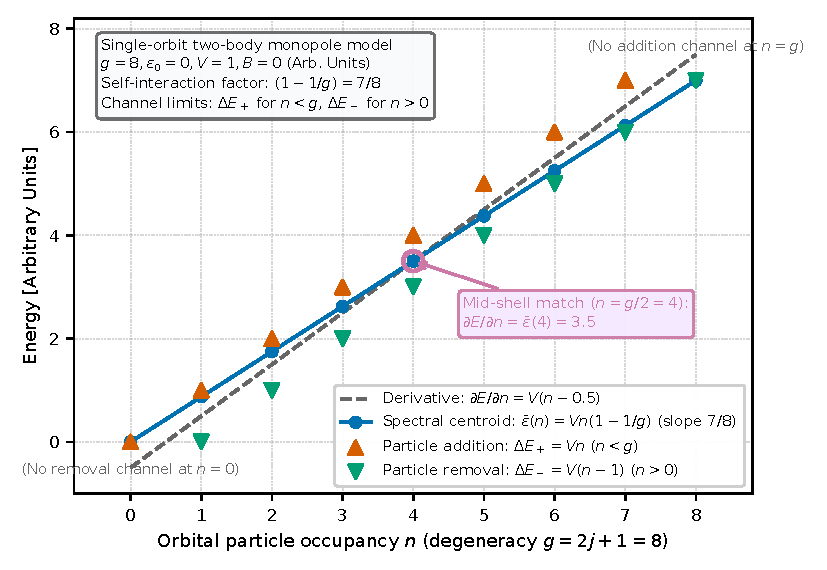
\includegraphics[width=0.85\textwidth]{Img/occupancy-centroids.pdf}
\caption{两体相互作用下的单轨道教学模型能量与重心演化对照示意图。设定轨道简并度 $g=8$，对比基准单粒子能 $e_0$、同轨两体单极相互作用强度 $w$ 与环境相互作用 $U$ 共同支配下，添粒能 $e^+$、移粒能 $e^-$、多项式连续能量导数 $\partial E/\partial n$ 以及加权谱重心 $e^{\mathrm{cent}}$ 随占据数 $n$ 的依赖关系。注意完整谱重心与连续导数在偏离半满壳层时存在本质差异（本图基于无额外多极关联的单轨两体代数模型，非真实原子核测量数据）。}
\label{fig:occupancy-centroids}
\end{figure}
}{}
%
}{%
    \section{壳结构、费米面与占据反馈 [未完成]}\label{sec:2-2}%
    \textit{本节尚未完成。}%
}

%-- Section 2.3: 配对、准粒子与阻塞
\setcounter{section}{2}%
\IfFileExists{Tex/Sections/sec-2-3.tex}{%
    \section{配对、准粒子与阻塞}\label{sec:2-3}


在低能核物理中，原子核不能简单视作各核子在静态平均场中独立运动的费米气体体系。由于核子—核子有效相互作用中短程吸引成分的存在，核子体系展现出显著的两体关联。在实验经验上，近稳定线已测量的绝大多数偶偶核基态均表现为自旋与宇称 $I^\pi = 0^+$，且其内禀破对激发能级通常明显高于邻近奇 $A$ 核的低能单粒子激发态；与此同时，结合能系统学呈现出普遍的奇偶交错效应。这些现象表明，同类核子之间存在强烈的超流配对倾向。为描述这种超越独立粒子平均场的集体效应，通常引入基于 Bardeen–Cooper–Schrieffer（BCS）理论的配对均场与准粒子方法\cite{book-suhonen-from-nucleons-to-nucleus, book-jain-nuclear-isomers}。

将配对微观理论应用于有限原子核体系，需要处理时间反演对称性、离散单粒子能级结构以及粒子数规范对称性破缺等一系列理论问题。本节系统阐述配对、准粒子与阻塞效应的微观机制：首先从时间反演轨道与短程吸引相互作用出发，分析偶偶核基态配对与奇偶质量差的微观成因，明确经验质量差与纯配对相互作用参数的物理边界；随后在平均粒子数约束变分框架下，给出 Bogoliubov–Valatin 正则变换、准粒子哈密顿量的 $2\times 2$ 矩阵化与对角化，讨论占据振幅、准粒子能量、自洽能隙方程与粒子数方程；进而辨析配对能隙、配对张量振幅与规范角三者的物理含义，说明均场粒子数破缺的理论属性，引出局域配对转动与粒子数投影接口；随后分析奇核子引起的泡利阻塞与自洽均场重排，探讨多准粒子态的形成机制并澄清静态 BCS 解在弱耦合下均场行为的物理本质；最后结合简化的两能级配对模型分析其临界解析行为与适用条件，阐明微观配对对集体动力学响应的调制作用。



\subsection{时间反演成对、短程吸引与奇偶效应的微观根源}\label{sec:2-3-1}


时间反演不变的平均场使半整数核子的单粒子轨道具有Kramers伙伴。先以球形场中的 $|k\rangle=|a,j,m_k\rangle$ 为例，a包含其它量子数；在轴对称变形场中，相应伙伴仍可定义，但j通常不再是好量子数。在常用的 Condon–Shortley 相位约定下\cite{book-suhonen-from-nucleons-to-nucleus}：
\begin{equation}\label{eq:2-3-1}
|\bar{k}\rangle \equiv \mathcal{T} |k\rangle = (-1)^{j - m_k} |a, -m_k\rangle.
\end{equation}
由于核子是自旋 $1/2$ 的费米子，重复作用时间反演算符满足 $\mathcal{T}^2 = -1$，保证了单粒子能级在无外加时间反演破缺场时至少具有二重 Kramers 简并。

当两个处于相互时间反演轨道的同类核子（质子—质子或中子—中子）发生相互作用时，在特定磁子能级对上产生对态 $c_k^\dagger c_{\bar{k}}^\dagger |0\rangle$。需要明确区分单个磁轨道对态与全壳层角动量耦合态的物理表示：单个固定磁投影的轨道对态 $c_k^\dagger c_{\bar{k}}^\dagger |0\rangle$ 仅具有总磁投影 $M = m_k + (-m_k) = 0$，在空间三维旋转下并非单一总角动量 $J$ 的本征态，而是包含了允许的总角动量 $J = 0, 2, 4, \dots$ 的线性叠加。在球对称单 $j$ 壳层中，将同壳层核子对严格耦合为总角动量为零的球形标量态时，需要对该壳层内所有磁子能级进行角动量张量耦合求和。在真空归一化约定下，归一化的双核子 $J=0$ 态为：
\begin{equation}\label{eq:2-3-2}
\begin{aligned}
|j^2; J=0, M=0\rangle &= \frac{1}{\sqrt{2(2j+1)}} \sum_{m=-j}^j (-1)^{j-m} c_{jm}^\dagger c_{j,-m}^\dagger |0\rangle \\
&= \frac{1}{\sqrt{\Omega}} \sum_{m>0} (-1)^{j-m} c_{jm}^\dagger c_{j,-m}^\dagger |0\rangle,
\end{aligned}
\end{equation}
其中 $\Omega = (2j+1)/2$ 为该单 $j$ 壳层的 Kramers 轨道对简并度。在轴对称形变核中，球形角动量 $J$ 被形变场破缺，但时间反演对称性依然保持，$c_k^\dagger c_{\bar{k}}^\dagger$ 对应于沿内禀对称轴投影 $K=0$ 的时间反演对产生算符。

反向运动的经典轨道可帮助形成成对的直觉，但不能单靠这幅图像证明任意两体作用的角动量排序。下面采用同类核子的吸引配对模型，主要保留时间反演轨道间的对散射。球形情况下，跨磁轨道的相干求和可以形成上述J=0对；实际相互作用还含其它角动量通道。实验奇偶效应为配对机制提供支持，具体强度仍取决于壳结构与所选相互作用\cite{book-suhonen-from-nucleons-to-nucleus, book-jain-nuclear-isomers}。

这种配对吸引直接反映在结合能的奇偶效应中。在偶偶核中，价核子以成对方式占据各能级；在奇 $A$ 核中，至少存在一个未配对的奇核子，该核子无法以同样方式形成时间反演基态对，导致奇 $A$ 核的总结合能系统性地低于相邻偶偶核的平均内插值；在奇奇核中，同时存在未成对的价质子与价中子，结合能进一步受损。在核质量实验数据分析中，常采用正束缚能 $B(N, Z) > 0$（结合越紧密数值越大）的离散差分公式来提取奇偶质量差。三点差分与四点差分公式定义为：
\begin{equation}\label{eq:2-3-3}
\Delta_B^{(3)}(N, Z) \equiv \frac{(-1)^{N+1}}{2} \left[ B(N-1, Z) - 2B(N, Z) + B(N+1, Z) \right],
\end{equation}
\begin{equation}\label{eq:2-3-4}
\Delta_B^{(4)}(N, Z) \equiv \frac{(-1)^N}{4} \left[ B(N-2, Z) - 3B(N-1, Z) + 3B(N, Z) - B(N+1, Z) \right].
\end{equation}
四点差分公式在结构上严格对应于相邻两个三点指标的对称中心平均：
\begin{equation}\label{eq:2-3-5}
\Delta_B^{(4)}(N, Z) = \frac{\Delta_B^{(3)}(N-1, Z) + \Delta_B^{(3)}(N, Z)}{2}.
\end{equation}
若设定束缚能包含平滑背景与纯奇偶交错项 $B(N) = B_{\mathrm{sm}}(N) + p(-1)^N$（$p > 0$），则上述带有 $(-1)^{N+1}$ 前置因子的三点式与四点式对纯交错项均给出一致的正能标 $+2p$（若改用总能量 $E = -B < 0$，则相应三点式前置因子调整为 $(-1)^N$）。

必须在物理上明确：\textbf{由实验结合能差分公式提取的经验奇偶质量差 $\Delta_B^{(3)}$ 或 $\Delta_B^{(4)}$，不能直接等同于微观哈密顿量中的纯配对能隙参数 $\Delta$。} 实验差分不仅包含配对关联能，还混杂了费米面附近离散单粒子能级间距 $(\epsilon_{k+1} - \epsilon_k)$、核子数变化引起的自洽均场重排能、形变平衡点的偏移以及单极势漂移等净贡献。在幻数闭壳邻近，差分主要反映单粒子能隙跳变；即使在开壳核区，将经验差分直接代入微观模型作为恒定配对参数也会忽略轨道依赖的能隙结构与极化响应。



\subsection{约束变分、Bogoliubov 变换与 BCS 均场推导}\label{sec:2-3-2}


为了在多体框架下统一处理配对关联，BCS 理论引入了破缺粒子数守恒的试探波函数。设单粒子产生算符为 $c_k^\dagger$，时间反演共轭算符为 $c_{\bar{k}}^\dagger$。为避免在配对求和中出现重复计数，指标 $k > 0$ 遍历半数单粒子态空间（例如在轴对称或球形基底下选取投影 $m_k > 0$）。定义单轨道对产生算符为 $P_k^\dagger \equiv c_k^\dagger c_{\bar{k}}^\dagger$。


\subsubsection{BCS 拟设与粒子数约束}\label{sec:2-3-bcs拟设与粒子数约束}


BCS 基态试探波函数假定时间反演轨道对处于独立相干凝聚态\cite{book-suhonen-from-nucleons-to-nucleus}：
\begin{equation}\label{eq:2-3-6}
|\mathrm{BCS}\rangle = \prod_{k>0} \left( u_k + v_k P_k^\dagger \right) |0\rangle = \prod_{k>0} \left( u_k + v_k c_k^\dagger c_{\bar{k}}^\dagger \right) |0\rangle,
\end{equation}
其中 $|0\rangle$ 为物理真空，$u_k$ 与 $v_k$ 为实变分参量。态矢的模方展开为 $\langle\mathrm{BCS}|\mathrm{BCS}\rangle = \prod_{k>0} (u_k^2 + v_k^2)$。乘积等于 1 本身在逻辑上并不能唯一推出每个因子独立等于 1；在理论中，我们将逐对归一化条件：
\begin{equation}\label{eq:2-3-7}
u_k^2 + v_k^2 = 1 \quad (\forall k > 0)
\end{equation}
确立为独立对振幅的标准规范化约定。在该约定下，$v_k^2$ 与 $u_k^2$ 分别代表轨道对 $(k, \bar{k})$ 被一对核子占据与未被占据的几率。

由于波函数展开包含具有不同偶数粒子数的态分量，$|\mathrm{BCS}\rangle$ 破缺了 $U(1)$ 粒子数规范对称性。为使该态对应特定核素的平均粒子数，需通过拉格朗日乘子 $\lambda$（化学势）引入变分约束：
\begin{equation}\label{eq:2-3-8}
\langle\mathrm{BCS}| \hat{n} |\mathrm{BCS}\rangle = \bar{n}, \quad \hat{n} = \sum_{k>0} \left( c_k^\dagger c_k + c_{\bar{k}}^\dagger c_{\bar{k}} \right).
\end{equation}
计算给出平均核子数关系式：
\begin{equation}\label{eq:2-3-9}
\bar{n} = 2 \sum_{k>0} v_k^2.
\end{equation}
式中因子 $2$ 源于每个轨道对包含两个时间反演态。需要强调的是，平均数约束 $\langle\hat{n}\rangle = \bar{n}$ 仅在期望值层面上控制粒子数，并不等于微观状态具有确定粒子数。


\subsubsection{Bogoliubov–Valatin 正则变换}\label{sec:2-3-bogoliubovvalatin正则变换}


定义准粒子产生与消灭算符如下\cite{book-suhonen-from-nucleons-to-nucleus}：
\begin{equation}\label{eq:2-3-10}
\alpha_k^\dagger = u_k c_k^\dagger - v_k c_{\bar{k}}, \quad \alpha_{\bar{k}}^\dagger = u_k c_{\bar{k}}^\dagger + v_k c_k,
\end{equation}
其厄米共轭为：
\begin{equation}\label{eq:2-3-11}
\alpha_k = u_k c_k - v_k c_{\bar{k}}^\dagger, \quad \alpha_{\bar{k}} = u_k c_{\bar{k}} + v_k c_k^\dagger.
\end{equation}
由逐对归一条件 $u_k^2 + v_k^2 = 1$ 可直接验证准粒子算符满足费米子反对易关系：
\begin{equation}\label{eq:2-3-12}
\{\alpha_k, \alpha_{k'}^\dagger\} = \delta_{kk'}, \quad \{\alpha_{\bar{k}}, \alpha_{\bar{k}'}^\dagger\} = \delta_{kk'}, \quad \{\alpha_k, \alpha_{k'}\} = 0.
\end{equation}
作用消灭算符于 BCS 基态可知 $\alpha_k |\mathrm{BCS}\rangle = 0$（$\forall k > 0$），因此 $|\mathrm{BCS}\rangle$ 即为无准粒子的准粒子真空态。


\subsubsection{辅助哈密顿量与 $2\times 2$ 矩阵结构}\label{sec:2-3-辅助哈密顿量与2times2矩阵结构}


考虑包含单粒子能量与对散射相互作用的模型纯配对哈密顿量：
\begin{equation}\label{eq:2-3-13}
\hat{H} = \sum_{k>0} \epsilon_k \left( c_k^\dagger c_k + c_{\bar{k}}^\dagger c_{\bar{k}} \right) - \sum_{k, l > 0} G_{kl} c_k^\dagger c_{\bar{k}}^\dagger c_{\bar{l}} c_l = \sum_{k>0} \epsilon_k \left( c_k^\dagger c_k + c_{\bar{k}}^\dagger c_{\bar{k}} \right) - \sum_{k, l > 0} G_{kl} P_k^\dagger P_l,
\end{equation}
其中相互作用矩阵元假定满足实对称 $G_{kl} = G_{lk} > 0$。引入平均粒子数约束后的辅助哈密顿量为 $\hat{H}' = \hat{H} - \lambda \hat{n}$。通过准粒子逆变换表达粒子算符：
\begin{equation}\label{eq:2-3-14}
c_k^\dagger = u_k \alpha_k^\dagger + v_k \alpha_{\bar{k}}, \quad c_{\bar{k}}^\dagger = u_k \alpha_{\bar{k}}^\dagger - v_k \alpha_k,
\end{equation}
并按准粒子正规积展开，辅助哈密顿量精确分解为：
\begin{equation}\label{eq:2-3-15}
\hat{H}' = H_0' + H_{11}' + H_{20}' + V_{\mathrm{RES}}.
\end{equation}
其中 $H_0' = \langle\mathrm{BCS}| \hat{H}' |\mathrm{BCS}\rangle$ 为基态平均能量；$H_{11}'$ 仅包含准粒子数算符项；$H_{20}'$ 包含成对产生或消灭准粒子的项；$V_{\mathrm{RES}}$ 包含四准粒子残余相互作用。

对哈密顿量中的配对两体相互作用项进行直接 Wick 收缩，保留完整的 $k=l$ 对角配对项及其平均场贡献，得到自洽自能修正：
\begin{equation}\label{eq:2-3-16}
\mu_k = G_{kk} v_k^2.
\end{equation}
进而定义相对于化学势与自能的单粒子有效能量：
\begin{equation}\label{eq:2-3-17}
\xi_k \equiv \epsilon_k - \lambda - \mu_k = \epsilon_k - \lambda - G_{kk} v_k^2,
\end{equation}
以及自洽配对能隙：
\begin{equation}\label{eq:2-3-18}
\Delta_k \equiv \sum_{l > 0} G_{kl} u_l v_l.
\end{equation}
在上述模型定义下，非对角的准粒子对产生项系数整齐表示为：
\begin{equation}\label{eq:2-3-19}
H_{20}' = \sum_{k>0} \left[ 2\xi_k u_k v_k - \Delta_k (u_k^2 - v_k^2) \right] \left( \alpha_k^\dagger \alpha_{\bar{k}}^\dagger + \alpha_{\bar{k}} \alpha_k \right).
\end{equation}
变分驻点条件要求能量对变分参量的一阶微商为零，等价于消除危险项系数 $H_{20}' \equiv 0$：
\begin{equation}\label{eq:2-3-20}
2\xi_k u_k v_k - \Delta_k (u_k^2 - v_k^2) = 0.
\end{equation}
在正能激发分支 $E_k > 0$ 且 $\Delta_k > 0$ 下，该条件与本任务所选取的准粒子相位约定相容，直接表述为正非对角元的 $2\times 2$ 厄米本征矩阵方程：
\begin{align}\label{eq:2-3-21}
\begin{pmatrix}
\xi_k & +\Delta_k \\
+\Delta_k & -\xi_k
\end{pmatrix}
\begin{pmatrix}
u_k \\
v_k
\end{pmatrix}
= E_k
\begin{pmatrix}
u_k \\
v_k
\end{pmatrix}.
\end{align}
对角化该矩阵给出特征方程 $E_k^2 - (\xi_k^2 + \Delta_k^2) = 0$，解得单准粒子激发能：
\begin{equation}\label{eq:2-3-22}
E_k = \sqrt{\xi_k^2 + \Delta_k^2}.
\end{equation}
第一行本征方程给出 $(\xi_k - E_k) u_k + \Delta_k v_k = 0$。结合逐对归一条件 $u_k^2 + v_k^2 = 1$，直接解出占据与非占据振幅：
\begin{equation}\label{eq:2-3-23}
v_k^2 = \frac{1}{2} \left( 1 - \frac{\xi_k}{E_k} \right), \quad u_k^2 = \frac{1}{2} \left( 1 + \frac{\xi_k}{E_k} \right), \quad u_k v_k = \frac{+\Delta_k}{2 E_k} > 0.
\end{equation}
必须指出：消去 $H_{20}'$ 仅保证能量泛函处于一阶变分驻点（stationarity），该解是否对应局域能量极小，还需检查约束允许方向上的二阶变分及竞争分支。QRPA频率、模范数与零模也要按同一稳定性合同解释，不能只看一组实频率。


\subsubsection{自洽能隙方程与粒子数方程}\label{sec:2-3-自洽能隙方程与粒子数方程}


将乘积项 $u_k v_k = \Delta_k / (2E_k)$ 代回配对能隙与粒子数定义式，给出在全系统中自洽保留自能 $\mu_k = G_{kk} v_k^2$ 的 BCS 方程组：
\begin{equation}\label{eq:2-3-24}
\Delta_k = \sum_{l > 0} G_{kl} \frac{\Delta_l}{2 \sqrt{\xi_l^2 + \Delta_l^2}}, \quad \xi_l = \epsilon_l - \lambda - G_{ll} v_l^2,
\end{equation}
\begin{equation}\label{eq:2-3-25}
\bar{n} = \sum_{k>0} \left( 1 - \frac{\xi_k}{\sqrt{\xi_k^2 + \Delta_k^2}} \right).
\end{equation}
若在活跃壳层内采用恒定配对相互作用力模型（$G_{kl} = G$），则自能为 $\mu_k = G v_k^2$，活跃轨道上的配对能隙统一为常数 $\Delta$，能隙方程严格写为：
\begin{equation}\label{eq:2-3-26}
\frac{2}{G} = \sum_{k>0} \frac{1}{\sqrt{(\epsilon_k - \lambda - G v_k^2)^2 + \Delta^2}}.
\end{equation}
上式约去了共同的非零 $\Delta$，因此不能用它排除或求出 $\Delta=0$ 支；零隙解应回到未约分的自洽方程处理。

在略去高阶准粒子残余相互作用 $V_{\mathrm{RES}}$ 的冻结独立准粒子近似下，两准粒子激发的能量满足 $E_k + E_l \ge 2\Delta$。这一 $2\Delta$ 是共同正能隙、冻结独立准粒子近似下的代数下界，并不要求连续谱；在实际原子核离散单粒子能级结构中，最低双准粒子激发由离散能级和 $E_{k_1} + E_{k_2}$ 决定，并受组态依赖的残余相互作用影响，并不必然等于常数 $2\Delta$。



\subsection{规范对称性破缺、配对转动与物理粒子数守恒}\label{sec:2-3-3}


BCS 理论将多体配对关联映射为非相互作用准粒子均场，但这种简化建立在破缺粒子数规范不变性的基础之上。理解该机制需要明确相关物理量的内涵及真实核体系的物理约束。


\subsubsection{能隙、配对张量与规范角}\label{sec:2-3-能隙配对张量与规范角}


在配对理论中，必须严格区分三个不同范畴的物理概念：
1. \textbf{配对能隙 $\Delta$：} 具有能量量纲（单位通常为 $\text{MeV}$）。它表征破裂一个核子对并激发两个独立准粒子所需的特征能标。
2. \textbf{配对张量振幅 $\kappa_k$：} 无量纲复数振幅，定义为在破缺粒子数参考态下的反常配对密度：
\begin{equation}\label{eq:2-3-27}
\kappa_k \equiv \langle\mathrm{BCS}| c_{\bar{k}} c_k |\mathrm{BCS}\rangle = u_k v_k = \frac{\Delta_k}{2 E_k}.
\end{equation}
   它表征特定轨道对在均场参考态下的凝聚振幅。这里需要区分定粒子数态与破缺参考态：\textbf{在守恒核子数 $N$ 的真实物理本征态 $|N\rangle$ 下，由于规范对称性保持，反常密度期望值恒等于零（$\langle N | c_{\bar{k}} c_k | N \rangle \equiv 0$）。} 这是因为算符 $c_{\bar{k}} c_k$ 改变体系总粒子数 2。非零反常密度用于表征选定规范取向的破缺参考态；在真实原子核态中，超流配对关联由粒子数守恒的两体密度矩阵关联 $\langle N | P_k^\dagger P_l | N \rangle$、双核子转移反应矩阵元 $\langle A+2 | P_k^\dagger | A \rangle$ 以及定数配对关联能来定量表征。
3. \textbf{配对规范角 $\theta$：} 全局粒子数规范变换群 $U(1)$ 的无量纲变换参量。在单粒子规范变换 $c_k \to e^{-i\theta} c_k$ 下，双核子湮灭算符变换为 $c_{\bar{k}} c_k \to e^{-2i\theta} c_{\bar{k}} c_k$。无量纲粒子数算符 $\hat{n}$ 在角表象下对应微分算符 $\hat{n} = -i \partial/\partial\theta$（不含 $\hbar$）。需要强调的是，准粒子无规相位近似（QRPA）中构造的局域共轭角算符是参考态局域切空间上的线性化描述，并不能推广为有限核完整 Hilbert 空间中满足严格全局对易关系的自伴量子力学角算符。


\subsubsection{均场破缺与局域配对转动}\label{sec:2-3-均场破缺与局域配对转动}


孤立原子核体系遵循严格的粒子数守恒定律（$[\hat{H}, \hat{n}] = 0$）。BCS 或 Hartree–Fock–Bogoliubov（HFB）参考态中出现的粒子数规范对称性破缺，是平均场变分近似处理复杂吸引配对相互作用的有效数学手段，不代表物理原子核发生真实的粒子数不守恒。

在自洽均场及残余响应保留相应对称性的理论极限中，破缺的连续规范对称性对应 Nambu–Goldstone（NG）零能模。Hinohara（2015）在线性响应理论框架下探讨了粒子数规范破缺态的零频响应\cite{hinohara-2015-nambu-goldstone-inertia-response}。在总能量 $E = -B_+$ 关于粒子数偏离的二次微商展开中：
\begin{equation}\label{eq:2-3-28}
E(N) = E(N_0) + \lambda \, \delta N + \frac{(\delta N)^2}{2 \mathcal{J}_{\text{pair}}} + \cdots,
\end{equation}
相应的正束缚能 $B_+(N) = -E(N)$ 展开式为：
\begin{equation}\label{eq:2-3-29}
B_+(N) = B_+(N_0) - \lambda \, \delta N - \frac{(\delta N)^2}{2 \mathcal{J}_{\text{pair}}} + \cdots,
\end{equation}
其中化学势为 $\lambda = \partial E/\partial N$，配对转动惯量定义为：
\begin{equation}\label{eq:2-3-30}
\mathcal{J}_{\text{pair}} \equiv \frac{\partial \bar{N}}{\partial \lambda} = -S(\hat{N}, \omega = 0) \quad (\text{单位：}\text{MeV}^{-1}).
\end{equation}
能面二次曲率满足 $\mathcal{J}_{\text{pair}}^{-1} = \partial^2 E/\partial N^2 = -\partial^2 B_+/\partial N^2$。此处始终以E表示内部总能，以$B_+$表示正束缚能；这一局部展开还要求指定平滑的自洽态族、固定其它粒子数的路径及非奇异响应。

必须明确区分两类物理转动惯量：\textbf{配对转动惯量 $\mathcal{J}_{\text{pair}}$ 的量纲是 $\text{MeV}^{-1}$，反映的是能量随粒子数规范变量变化的微观曲率响应；而空间三维集体转动惯量 $\mathcal{J}_{\text{space}}$ 的量纲为 $\hbar^2/\text{MeV}$（或记为 $\text{MeV}^{-1}\hbar^2$），反映的是孤立体系绕真实空间几何轴旋转的动能响应。二者对应的微观自由度与动力学机制完全不同，绝对不能因名称相似而混同。}

为了消除均场近似引入的粒子数弥散，理论上采用粒子数投影（Particle Number Projection, PNP）方法，通过对规范角进行闭合积分：
\begin{equation}\label{eq:2-3-31}
\hat{P}_N = \frac{1}{2\pi} \int_0^{2\pi} e^{i (\hat{n} - N) \theta} \mathrm{d}\theta,
\end{equation}
从试探波函数中滤出具有好粒子数的分量 $|N\rangle \propto \hat{P}_N |\mathrm{BCS}\rangle$。需要指出的是，投影后的状态消除了解中的粒子数涨落，属于好粒子数近似态，但由于其试探波函数形式仍受限于投影前的变分空间，通常并不等同于完整多体哈密顿量的严格本征态。这一内禀参考态与对称性恢复的逻辑，构成了后续处理空间旋转对称性恢复（角动量投影）的方法范式。



\subsection{阻塞效应与多准粒子态的微观重排}\label{sec:2-3-4}


当原子核处于奇 $A$ 核、奇奇核或偶偶核的断对激发态时，体系包含未成对的单粒子。这些未配对核子对周围核子介质的配对散射产生显著的排斥与阻碍作用，即阻塞效应（blocking effect）\cite{book-jain-nuclear-isomers}。


\subsubsection{泡利阻塞与自洽重排}\label{sec:2-3-泡利阻塞与自洽重排}


设某一特定的单核子态 $|k_b\rangle$ 已被一个奇准粒子单独占据。根据费米子泡利不相容原理：
1. 任何其他同类核子均无法再填入该态 $|k_b\rangle$；
2. 原本对应的时间反演轨道对 $(k_b, \bar{k}_b)$ 无法再容纳双核子成对凝聚；
3. 双核子配对散射相互作用中，所有涉及轨道 $k_b$ 的对散射矩阵元被全部阻断。

因此，轨道 $k_b$ 被从活跃的配对相互作用空间中剔除。在自洽计算中，该态的自洽能隙方程与粒子数方程变为：
\begin{equation}\label{eq:2-3-32}
\Delta_k = \sum_{l > 0, l \ne k_b} G_{kl} \frac{\Delta_l}{2 \sqrt{\xi_l^2 + \Delta_l^2}},
\end{equation}
\begin{equation}\label{eq:2-3-33}
\bar{n} - 1 = \sum_{k>0, k \ne k_b} \left( 1 - \frac{\xi_k}{\sqrt{\xi_k^2 + \Delta_k^2}} \right).
\end{equation}
当被阻塞的轨道位于费米面附近时，该能级本应对配对能隙方程提供较大贡献。将其剔除后，自洽求解得到的有效配对能隙 $\Delta$ 出现局域减小。与此同时，奇核子占据引起的势场变化与粒子数守恒要求，会驱动周围非阻塞轨道的化学势 $\lambda$ 与占据几率 $v_k^2$ 发生自洽调整，引起核芯的极化重排效应\cite{book-jain-nuclear-isomers}。


\subsubsection{多准粒子态与高 $K$ 异能态机制}\label{sec:2-3-多准粒子态与高k异能态机制}


在形变核区，当体系具有良好的轴对称性（或接近轴对称）且破坏轴对称性的耦合或 Coriolis 混合较弱时，单粒子角动量在对称轴上的投影量子数 $\Omega$ 近似为守恒量；若核体系显著偏离轴对称（具有显著三轴形变），$\Omega$ 通常发生混合，轴投影不再是良好量子数。在近轴对称条件下断开多个时间反演对时，可以激发多个准粒子，其单粒子轴投影平行极化耦合形成较大的总内禀角动量投影 $K = \sum_i \Omega_i$\cite{book-jain-nuclear-isomers}。

在多准粒子态激发能估算中，通常表示为各准粒子能量、核芯转动能与两体残余作用贡献的叠加\cite{book-jain-nuclear-isomers}：
\begin{equation}\label{eq:2-3-34}
E(K) = E_0 + \sum_{i\in\mathrm{qp}} E_{\mathrm{qp}}(i) + E_{\mathrm{rot}} + \Delta E_{\mathrm{residual}}.
\end{equation}
当多个高投影轨道同时被单粒子占据时，多个配对散射通道被同步阻断，在相对较低的激发能量下形成高 $K$ 构型。需要指出的是，高 $K$ 态形成长寿命同核异能态的关键，不仅在于多准粒子态的能量稳定性，更在于其向低 $K$ 基态带退激时必须跨越巨大的 $K$ 量子数差（$\Delta K$），受到电磁辐射选择定则的极强跃迁阻碍（$K$ 禁戒跃迁阻碍）；阻塞机制解释了多准粒子态在能谱中的形成与局域能隙减弱，而长半衰期的产生还取决于该阻碍机制与退激通道的动力学特征（例如 $^{178}\mathrm{Hf}$ 中的 $16^+$ 态半衰期达 $T_{1/2} \approx 31\text{ 年}$，其具体跃迁矩阵元与寿命分析将在后续章节专门展开）。


\subsubsection{阻塞状态下的配对残留与均场近似边界}\label{sec:2-3-阻塞状态下的配对残留与均场近似边界}


关于多准粒子态与阻塞效应，需要确立客观的理论适用界限：

首先，阻塞若干个特定单粒子轨道虽然削弱了局域配对能隙，但未被阻塞的其他价轨道仍然在费米面两侧参与配对散射。即便在四准粒子或六准粒子激发态中，剩余轨道仍可能维持配对关联，其大小须在指定相互作用和组态下计算。不能断言多准粒子态的微观配对完全消失，也不能将多准粒子态的微观转动惯量直接等同为无配对的理想刚体转动惯量。

其次，静态BCS的非零能隙解可能在临界强度或旋转条件下消失，这不等于粒子数守恒体系的全部配对关联同时消失。下面的两壳例子给出连续趋零的能隙，而其它自洽分支也可能发生交叉或跳变。有限核没有无限体系的热力学极限，仍可有精确能级交叉和选支后的非解析行为。粒子数投影、精确对角化或更广的动力学描述可检验均场遗漏的关联；它们不保证所有路径都平滑，也不能仅由弱配对便断言存在强烈的配对振动。



\subsection{解析控制：两能级教学极限与集体响应的配对反馈}\label{sec:2-3-5}


为了在可控模型下检验均场配对解的临界行为，考察简化的两能级配对模型空间。该模型允许推导精确的解析表达式，用于展示变分解的数学结构及其局限性。


\subsubsection{两能级模型在纯配对哈密顿量下的解析推导}\label{sec:2-3-两能级模型在纯配对哈密顿量下的解析推导}


设模型空间仅包含两个能级，单粒子能量分别为 $\epsilon_1 = -\frac{1}{2}\varepsilon$ 与 $\epsilon_2 = +\frac{1}{2}\varepsilon$，能级间距为 $\varepsilon$。每个壳层的轨道对简并度均为 $\Omega = (2j+1)/2$。设体系的平均粒子数严格等于单个能级的容量，即 $\bar{n} = 2\Omega$（半填充条件）。在无相互作用时，下能级完全被 $2\Omega$ 个核子填满（$v_1 = 1, v_2 = 0$），上能级完全为空。

在本任务采用的纯配对哈密顿量 $\hat{H} = \sum \epsilon_k n_k - G \sum_{k, l} P_k^\dagger P_l$ 下，保留完整的对角项与其 Wick 自能修正 $\mu_i = G v_i^2$。定义上下两能级的占据差参量 $t \equiv v_1^2 - v_2^2$。由粒子—空穴对称性与粒子数守恒要求 $v_1^2 + v_2^2 = 1$，得到 $v_1^2 = (1+t)/2$ 与 $v_2^2 = (1-t)/2$。

在这条镜像对称的BCS积态路径上，直接计算能量期望得到
\begin{equation}\label{eq:2-3-35}
\mathcal E(t)=-\Omega\varepsilon t-G\left[\Omega+\frac{(4\Omega^2-2\Omega)(1-t^2)}4\right].
\end{equation}
其一阶导数为 $-\Omega\varepsilon+G\Omega(2\Omega-1)t$，因此内部驻点满足：
\begin{equation}\label{eq:2-3-36}
t_* = \frac{\varepsilon}{G(2\Omega - 1)}.
\end{equation}
在非零配对且保持镜像对称的驻点上，自洽化学势为 $\lambda = -\frac{G}{2}$，有效单粒子能量满足：
\begin{equation}\label{eq:2-3-37}
|\xi_1| = |\xi_2| = \frac{\Omega \varepsilon}{2\Omega - 1}.
\end{equation}
非零能隙方程在两壳各计 $\Omega$ 对轨道，给出 $1=G\Omega/E$，故准粒子能量为：
\begin{equation}\label{eq:2-3-38}
E_1 = E_2 = E = \Omega G.
\end{equation}
进而解出配对能隙的解析表达式：
\begin{equation}\label{eq:2-3-39}
\Delta = \sqrt{E^2 - \xi^2} = \Omega G \sqrt{1 - t_*^2} = \Omega G \sqrt{1 - \left[ \frac{\varepsilon}{G(2\Omega - 1)} \right]^2} \quad (G > G_{c,\mathrm{pair}}).
\end{equation}
临界配对相互作用强度为：
\begin{equation}\label{eq:2-3-40}
G_{c,\mathrm{pair}} = \frac{\varepsilon}{2\Omega - 1}.
\end{equation}
在非零配对支（$G > G_{c,\mathrm{pair}}$）上，占据几率为：
\begin{equation}\label{eq:2-3-41}
v_1^2 = \frac{1}{2} \left[ 1 + \frac{\varepsilon}{G(2\Omega - 1)} \right], \quad v_2^2 = \frac{1}{2} \left[ 1 - \frac{\varepsilon}{G(2\Omega - 1)} \right].
\end{equation}
此处给出明确说明：Suhonen 专著第 13.5 节（印刷本第 408–410 页）得到的临界强度为 $2\varepsilon/(4\Omega - 1)$，其分母多出的因子源于 Suhonen 所采用的哈密顿量不仅包含时间反演轨道对的单极散射，还包含了所有壳层指标 $a,b,c,d \in \{1,2\}$ 耦合为 $J=0$ 的广义两体矩阵元，从而在自能中引入了额外的跨壳粒子—空穴收缩贡献；完整对账与模型映射留待附录 B。上述解析解是在本节正文明确规定的纯配对相互作用哈密顿量与自能约定下的严格推导结果。


\subsubsection{极限检验与临界条件}\label{sec:2-3-极限检验与临界条件}


利用上述解析表达式可清晰考察变分解的极限性质：
1. \textbf{临界阈值与连续消失：} 当相互作用强度从上方逼近临界点 $G \downarrow G_{c,\mathrm{pair}}$ 时，由于根式行为 $\Delta \sim \Omega G \sqrt{2(G - G_c)/G_c}$，能隙 $\Delta$ 连续趋近于零。当 $G \le G_{c,\mathrm{pair}}$ 时，能隙方程无非平凡实根，$\Delta \equiv 0$，此时占据几率退化为平庸的 $v_1 = 1, v_2 = 0$，体系回到无配对均场的基态。
2. \textbf{区分临界极限与无相互作用极限：} 必须明确区分能隙消失的临界极限与无两体作用极限。当 $G \to G_{c,\mathrm{pair}}^+$ 时，均场配对能隙 $\Delta \to 0$，但此时两体配对相互作用强度 $G_{c,\mathrm{pair}} > 0$ 仍为有限正值，体系在对角部分仍包含两体残余作用；真正的无相互作用极限对应 $G \to 0$。将二者混淆会误判临界区附近的相互作用属性。
3. \textbf{强配对极限（$G/\varepsilon \to \infty$）：} 当 $G/\varepsilon \gg 1$ 时，$t_* \to 0$，占据几率趋于均分 $v_1^2 \to 1/2, v_2^2 \to 1/2$。此时能隙与相互作用强度之比趋于饱和比值 $\Delta / G \to \Omega$。

两能级模型是用于概念检验的高度简化模型，其解析解反映的是特定简并空间与恒定配对矩阵元假定下的数学特征，不能作为实际原子核结构计算的直接结果。 在真实核体系中，单粒子能级呈现不均匀分布与形变劈裂，且残余相互作用包含高阶多极分量，其实际演化受复杂组态混合控制。


\subsubsection{配对对集体转动与动态响应的微观反馈}\label{sec:2-3-配对对集体转动与动态响应的微观反馈}


在微观多体框架下，超流配对关联对核体系的宏观集体运动具有关键的调制作用：
1. \textbf{两准粒子激发阈值的施加：} 准粒子能量满足 $E_k = \sqrt{\xi_k^2 + \Delta_k^2} \ge \Delta_k$，使得费米面附近的内禀两准粒子激发能受到能隙推高。这可以拉开部分集体态与内禀二准粒子组态的能标；实际阻尼还取决于耦合矩阵元与可用相空间；
2. \textbf{跃迁相干因子调制：} 在准粒子表象下展开单体电磁与多极跃迁算符时，由于配对产生的粒子与空穴成分之间的量子干涉，跃迁矩阵元乘上了相干因子 $(u_k v_{k'} \mp v_k u_{k'})$\cite{book-suhonen-from-nucleons-to-nucleus}。这导致不同多极跃迁的响应截然不同，部分多极跃迁受到相干增强，而另一些则受到抑制；
3. \textbf{转动惯量的微观抑制：} 在 Inglis–Belyaev 显式曲率公式中，转动惯量分量由角动量算符在准粒子基底下的矩阵元除以双准粒子激发能给出，其表达式受两准粒子能量分母 $E_k + E_{k'}$ 增大与相干因子干涉的双重压低，能够改变转动惯量；无配对极限仍保留壳结构与响应效应，并不自动等于经典刚体值。

然而，在动力学层面必须明确：\textbf{集体转动惯量是单粒子轨道能级、配对能隙、形状形变度以及多极残余相互作用联合贡献的微观响应结果，改变配对能隙并不单一决定转动惯量的变化；在没有完整自洽微观动力学计算的前提下，不能简单将转动惯量的偏离唯一归因于配对的消失。} 这些概念为后续章节讨论三维旋转、微观惯量张量与形状动力学提供了自洽的微观出发点。
%
}{%
    \section{配对、准粒子与阻塞 [未完成]}\label{sec:2-3}%
    \textit{本节尚未完成。}%
}

%-- Section 2.4: 形状坐标、测度与集体量子化
\setcounter{section}{3}%
\IfFileExists{Tex/Sections/sec-2-4.tex}{%
    \section{形状坐标、测度与集体量子化}\label{sec:2-4}


第 1.2 节已经说明，强四极关联可以与 $I=0$ 态的球对称实验室一体密度并存。形变参考构型描述的是内部关联的一种组织方式，集体波函数则给出这些构型的量子叠加。这里进一步追问：选取形状和取向作为坐标以后，应怎样计算运动能量，又怎样解释波函数在形状空间中的分布？

本节先采用常正质量参数 $B$、五维欧氏四极坐标的教学 Bohr 模型。它使坐标、动能与积分测度之间的关系能够逐步推导；随后再说明一般惯性函数与量子化方案增加了哪些输入。五个坐标只保留四极自由度，并不完整表征核密度中的径向变化、高阶多极分量或质子—中子分布差异。


\subsection{从五个实坐标到形状与取向}\label{sec:2-4-1}


用无量纲球张量 $\alpha_{2\mu}$ 描述所选集体构型，其分量满足实条件

\begin{equation}\label{eq:2-4-1}
\alpha_{2\mu}^{*}=(-1)^\mu\alpha_{2,-\mu}.
\end{equation}

因此五个复球分量只含五个独立实自由度。为使欧氏范数显式成立，可选择

\begin{equation}\label{eq:2-4-2}
q_0=\alpha_{20},\qquad
q_{\mu c}=\sqrt{2}\operatorname{Re}\alpha_{2\mu},\qquad
q_{\mu s}=\sqrt{2}\operatorname{Im}\alpha_{2\mu},
\quad \mu=1,2.
\end{equation}

这五个实坐标满足 $\sum_a q_a^2=\sum_{\mu=-2}^{2}|\alpha_{2\mu}|^2$。其中 $\sqrt{2}$ 补偿了正、负磁分量在球张量范数中的成对贡献，速度范数也遵循同一关系。它们是集体构型的坐标，而非精确核态实验室密度的五个非零期望值。

例如，集体波函数可在许多取向的形变构型上都有振幅；恢复旋转对称性后，一体密度仍可为球对称。因此，从实验室态进入内禀坐标，并不是给核态指定一只已固定朝向的椭球。内禀坐标也可用来描述宽分布与振动，只有在分布足够局域时，单个参考构型才可能有效概括该态。

四极张量也可表示为实对称无迹矩阵。选其本征轴为内禀主轴，在这个坐标系中，球分量可取为

\begin{equation}\label{eq:2-4-3}
a_{\pm1}=0,\qquad
a_0=\beta\cos\gamma,\qquad
a_{+2}=a_{-2}=\frac{\beta\sin\gamma}{\sqrt{2}}.
\end{equation}

三个 Euler 角 $\Omega=(\phi,\theta,\psi)$ 描述主轴系相对于实验室系的取向；按本文的旋转约定，$\alpha_{2\mu}=\sum_\nu D^2_{\mu\nu}(\Omega)a_\nu$。由 $D^2$ 的幺正性，

\begin{equation}\label{eq:2-4-4}
\sum_{\mu=-2}^{2}|\alpha_{2\mu}|^2=a_0^2+2a_2^2=\beta^2.
\end{equation}

$\beta$ 因而是所选四极坐标的幅度，$\gamma$ 则给出内禀平面中的极角。这是坐标参数化，不是平移，也没有预先假定形状与取向的运动彼此独立。Bohr 原作以小幅核表面形变建立这一变换；它同样提示，具体密度与几何表面的对应仍有模型条件\cite{bohr-1952-surface-particle-coupling}。

主轴系并不唯一。一般三轴构型有六种轴序，每种轴序又有四种保持右手性的方向选择，共有 24 种等价重标记。它们组成旋转群 $O$，通过形状参数和 Euler 角的联合变换保持实验室四极张量不变。本文选择 $\beta\ge0$、$0\le\gamma\le\pi/3$ 作为形状扇区；六个形状扇区间的关系来自轴置换，不需要再借助空间反演。

对于固定轴序、三个本征值不同的构型，绕各主轴转动 $\pi$ 仍保持张量不变。这四种操作构成稳定子 $D_2$，所以限制形状扇区后，Euler 取向仍有这一冗余。若把空间反演也计入四极椭球的点对称操作，则得到八阶群 $D_{2h}$；它与 24 重主轴重标记具有不同含义。在轴对称端点，绕对称轴的连续旋转使稳定子进一步扩大；在 $\beta=0$，全部取向及 $\gamma$ 都失去唯一含义\cite{bohr-1952-surface-particle-coupling, prochniak-rohozinski-2009-bohr-collective-hamiltonian}。

下文固定轴号 $k=1,2,3$ 分别对应 $x',y',z'$。在小幅表面形变的轴长映射下，$\gamma=0$ 是以 $z'$ 为对称轴的长椭球端点，$\gamma=\pi/3$ 是以 $y'$ 为对称轴的扁椭球端点。$\gamma=\pi/6$ 是本文扇区的中点，三个轴通常不同；“中点”本身不定义适用于所有模型的最大三轴性量度。


\subsection{形状依赖的经典动能}\label{sec:2-4-2}


常 $B$ 模型从五个实欧氏坐标的动能出发：

\begin{equation}\label{eq:2-4-5}
T=\frac{B}{2}\sum_a\dot q_a^2
=\frac{B}{2}\sum_{\mu=-2}^{2}|\dot\alpha_{2\mu}|^2.
\end{equation}

对 $\alpha=D^2a$ 求时间导数，一部分来自 $a$ 的变化，另一部分来自主轴系旋转。主轴条件使这两类速度的内积为零。由于

\begin{equation}\label{eq:2-4-6}
\dot a_0^2+2\dot a_2^2=\dot\beta^2+\beta^2\dot\gamma^2,
\end{equation}

动能可写为

\begin{equation}\label{eq:2-4-7}
T=\frac{B}{2}\left(\dot\beta^2+\beta^2\dot\gamma^2\right)
+\frac12\sum_{k=1}^{3}\mathcal J_k(\beta,\gamma)\omega_k^2.
\end{equation}

这里 $\omega_k$ 是角速度在内禀主轴上的分量。没有形状速度与取向速度的交叉项，是这个二次型的性质；$\beta^2\dot\gamma^2$ 和形状依赖的 $\mathcal J_k$ 仍把各运动联系起来，不能据此把波函数普遍分解为互不耦合的因子\cite{bohr-1952-surface-particle-coupling}。

其物理意义可以从形状变化看出：即便某时刻只改变 $\beta$，转动惯量也随之变化，已有角动量对应的转动能因此改变。反过来，在给定角动量的通道中，不同构型的转动能会影响形状分布。把形状振动与转动写成两项，帮助辨认各类运动的来源，并不消除这种反馈。若要冻结形状，需再引入相应的近似。

转动几何因子可先从第三轴看出。绕 $z'$ 的微小转动使分量 $a_\nu$ 获得相位 $e^{-i\nu\,\delta\chi}$，因此相应速度范数的系数为 $\sum_\nu\nu^2|a_\nu|^2=8a_2^2$，得到 $\mathcal J_3=4B\beta^2\sin^2\gamma$。另两轴通过轴置换得到

\begin{equation}\label{eq:2-4-8}
\mathcal J_k=4B\beta^2\sin^2\left(\gamma-\frac{2\pi k}{3}\right),
\qquad k=1,2,3.
\end{equation}

这也是 Bohr 小幅、不可压缩无旋流模型中的惯量形式。它不是实核三条惯量的普遍经验定律。以 $\gamma=0$ 为例，$\mathcal J_3=0$、$\mathcal J_1=\mathcal J_2=3B\beta^2$；零分量反映绕对称轴改变取向不改变这个表面构型，不是说真实核不能拥有沿该轴的微观角动量\cite{bohr-1952-surface-particle-coupling}。

$\beta$、$\gamma$ 和 Euler 角均无量纲，故 $[B]=\text{能量}\times\text{时间}^2=\hbar^2/\text{能量}$，$\mathcal J_k$ 具有同一单位。用 $\hat j_k=\hat J_k/\hbar$ 表示无量纲角动量，可避免在转动能中遗漏 $\hbar^2$。这些惯量单位与电四极矩的电荷、长度平方单位无关。


\subsection{量子动能与积分测度}\label{sec:2-4-3}


常 $B$ 模型的量子动能在原实坐标中已经确定为 Cartesian Laplacian：

\begin{equation}\label{eq:2-4-9}
\hat T=-\frac{\hbar^2}{2B}\sum_a\frac{\partial^2}{\partial q_a^2}.
\end{equation}

设新坐标为 $y^i=(\beta,\gamma,\phi,\theta,\psi)$，将欧氏线元记为 $\sum_a\mathrm dq_a^2=h_{ij}\mathrm dy^i\mathrm dy^j$，其中 $h_{ij}$ 不含常数 $B$，$h^{ij}$ 为其逆矩阵。同一算符的坐标变换为

\begin{equation}\label{eq:2-4-10}
\hat T=-\frac{\hbar^2}{2B}
\frac{1}{\sqrt h}\sum_{i,j}
\frac{\partial}{\partial y^i}
\left(\sqrt h\,h^{ij}\frac{\partial}{\partial y^j}\right),
\qquad h=\det(h_{ij}).
\end{equation}

这是 Laplace–Beltrami 形式。度规系数随坐标变化，不会使原来平直的五维空间产生内禀曲率；此处的几何因素来自坐标网格。若另从一般坐标相关的经典质量张量出发，Podolsky–Pauli 构造是一种需要声明的量子化选择，不能仅由经典动能唯一指定全部量子修正\cite{prochniak-rohozinski-2009-bohr-collective-hamiltonian}。

从主轴本征值差得到的 Jacobian 含 $\beta^3|\sin3\gamma|$，内禀平面的极坐标变换再贡献一个 $\beta$；Euler 角则贡献旋转群的 Haar 因子 $\sin\theta$。吸收整体常数后，本节采用

\begin{equation}\label{eq:2-4-11}
\mathrm d\tau=\beta^4|\sin3\gamma|\,\mathrm d\beta\,\mathrm d\gamma\,\mathrm d\Omega,
\qquad
\mathrm d\Omega=\sin\theta\,\mathrm d\phi\,\mathrm d\theta\,\mathrm d\psi.
\end{equation}

若将 $B$ 纳入质量度规，其体积元还带常数 $B^{5/2}$；主轴重复覆盖及 Haar 元的整体归一也带常数。这些可一致吸收到波函数归一中，不改变概率，不能同坐标相关权重混淆\cite{prochniak-rohozinski-2009-bohr-collective-hamiltonian}。

在所选扇区内部，动能写为 $\hat T_{\mathrm{vib}}+\hat T_{\mathrm{rot}}$，其中

\begin{equation}\label{eq:2-4-12}
\hat T_{\mathrm{vib}}=-\frac{\hbar^2}{2B}
\left[
\frac{1}{\beta^4}\frac{\partial}{\partial\beta}
\left(\beta^4\frac{\partial}{\partial\beta}\right)
+
\frac{1}{\beta^2\sin3\gamma}\frac{\partial}{\partial\gamma}
\left(\sin3\gamma\frac{\partial}{\partial\gamma}\right)
\right],
\end{equation}

\begin{equation}\label{eq:2-4-13}
\hat T_{\mathrm{rot}}=\sum_{k=1}^{3}\frac{\hat J_k^2}{2\mathcal J_k}
=\frac{\hbar^2}{8B\beta^2}
\sum_{k=1}^{3}\frac{\hat j_k^2}
{\sin^2(\gamma-2\pi k/3)}.
\end{equation}

$\hbar^2/B$ 提供能量单位，其余导数和 $\beta$ 的幂次均无量纲。尤其 $1/\beta^2$ 是幅度依赖的几何因子，不能解释成物理长度平方的倒数。加上 $V(\beta,\gamma)$ 后，形状与取向仍通过同一哈密顿量决定量子态。

径向部分展开为 $\partial_\beta^2+(4/\beta)\partial_\beta$。第二项记录了随幅度增长的四维角向体积，不能在换坐标时省去。若只把笛卡尔动量换成 $-i\hbar\partial_\beta$ 后平方，就会得到另一种微分算符，并破坏它与所选内积的配合。体积元因而同时参与波函数归一和动能构造，不只是画概率图时的附加权重。

一般 Bohr 模型需要更多微观输入。Próchniak 与 Rohoziński 在综述中用三个振动惯性函数和三个转动惯性函数描述经典二次动能；它们通常依赖于形变坐标 $(\beta, \gamma)$。在由一般经典质量张量构造量子哈密顿量时，必须将平直欧氏空间坐标微分产生的几何因子 $\beta^4 |\sin 3\gamma|$，与依赖于动力学微观响应的质量张量行列式 $\sqrt{\det B(\beta, \gamma)}$ 严格区分开来。在 Podolsky–Pauli 构造下，内积权重与坐标依赖质量张量相耦合；而在更广泛的唯象或自洽集体模型中，动能二阶微分算符的逆质量系数张量与积分测度中的标量权重函数 $W(\beta, \gamma)$ 甚至可以独立指定，前一种关联仅为其特殊极限。在处理一般微观坐标依赖质量时，绝不能不加检验地直接沿用常 $B$ 模型下无额外质量权重的几何内积；具体一般形式与量子势修正留待附录 C 展开\cite{prochniak-rohozinski-2009-bohr-collective-hamiltonian}。


\subsection{坐标端点与波函数定义域}\label{sec:2-4-4}


采用上述归一约定，常 $B$ 模型的波函数满足

\begin{equation}\label{eq:2-4-14}
\int|\Psi(\beta,\gamma,\Omega)|^2
\beta^4|\sin3\gamma|\,\mathrm d\beta\,\mathrm d\gamma\,\mathrm d\Omega=1.
\end{equation}

在这个模型中，关于 $\gamma$ 的边缘概率密度还需积分掉 $\beta$ 和取向，并乘上 $|\sin3\gamma|$。单独画出 $|\Psi|^2$，尚不能把纵轴称为相对于 $\mathrm d\gamma$ 的概率密度。

取向与形状相关时，这一积分也包含不同转动分量的贡献，不能先假定波函数可分离再解释角分布。这里的概率是所选集体模型中的坐标概率；把它同电荷不变量、寿命或跃迁强度连接起来，还要指定相应算符，不能将模型边缘分布直接称为实验测得的连续核密度。

轴对称端点的 Jacobian 为零，表示部分取向坐标退化，不能据此添上一道物理硬壁。要使量子动能自伴，除微分表达式外，还要指定定义域，并使分部积分的边界形式在域内任意两个函数之间消失。有限概率流甚至某个态的零概率流，都不足以独自确定唯一自伴域。

对标量角向算符，该边界形式正比于 $\sin3\gamma\,[f^*g'-(f')^*g]$ 在两端的差，其中撇号表示对 $\gamma$ 求导。要求它对定义域中的任意 $f,g$ 都消失，比只考察一个波函数的流更强；还须使所选算符域与其伴随的域相配。这说明边界条件属于模型的量子定义，而非从测度归零直接读出的数值便利。

以 $I=0$、平坦角向势的标准正则分支为例，令 $x=\cos3\gamma$，则

\begin{equation}\label{eq:2-4-15}
\frac{1}{\sin3\gamma}\frac{\mathrm d}{\mathrm d\gamma}
\left(\sin3\gamma\frac{\mathrm d}{\mathrm d\gamma}\right)
=9\frac{\mathrm d}{\mathrm dx}
\left[(1-x^2)\frac{\mathrm d}{\mathrm dx}\right].
\end{equation}

相应正则本征函数是 $P_\ell(x)$，算符本征值为 $-9\ell(\ell+1)$。它们满足端点条件 $\sin3\gamma\,\mathrm d\psi/\mathrm d\gamma\to0$，同时 $P_\ell(\pm1)=(\pm1)^\ell$ 可以非零。这里选择的是由原坐标中正则波函数继承的分支，不是为所有集体问题证明了同一个边界条件\cite{bohr-1952-surface-particle-coupling}。

有转动分量时，还须满足主轴重标记的一致性，不能把所有分量一律置零。对于偶偶核的纯四极标量集体空间，$D_2$ 对称化可限制 Wigner 函数展开只含偶数 $K$；$K$ 在这里是所选主轴上的展开标签，三轴哈密顿量一般会混合这些分量，并不赋予全局好 $K$。在 $\beta=0$，不同角向通道也须共同恢复正则五维函数。加入奇核子或其它内禀自由度后，应重新构造包含它们的变换性质和定义域。


\subsection{平均形状角与动力学能标}\label{sec:2-4-5}


$V(\beta,\gamma)=V(\beta)$ 只说明势不依赖 $\gamma$，不表示哈密顿量在 $\gamma$ 平移下不变；动能中仍有 $\sin3\gamma$。在常 $B$ 模型的标准最低角向 $I=0$ 通道中，常数函数使非负角向动能达到零，因而成为这一通道的基态。

为单独观察角向分布，现限制在 $\beta=\beta_0>0$ 的角向模型上。这是受约束流形，不是将 $\delta(\beta-\beta_0)$ 当作完整五维可归一径向波函数。令 $M_\gamma=B\beta_0^2$，其平坦势动能为

\begin{equation}\label{eq:2-4-16}
\hat H_\gamma=-E_*\frac{1}{\sin3\gamma}\frac{\mathrm d}{\mathrm d\gamma}
\left(\sin3\gamma\frac{\mathrm d}{\mathrm d\gamma}\right),
\qquad E_*=\frac{\hbar^2}{2M_\gamma}.
\end{equation}

在 $\int_0^{\pi/3}|\psi|^2\sin3\gamma\,\mathrm d\gamma=1$ 的约定下，常数基态为 $\psi_0=\sqrt{3/2}$。变量变换需保留积分方向：

\begin{equation}\label{eq:2-4-17}
\mathrm dx=-3\sin3\gamma\,\mathrm d\gamma,\qquad
\int_0^{\pi/3}f(\cos3\gamma)\sin3\gamma\,\mathrm d\gamma
=\frac13\int_{-1}^{1}f(x)\,\mathrm dx.
\end{equation}

故 $p_x(x)=1/2$，而 $p_\gamma(\gamma)=(3/2)\sin3\gamma$。同一态在 $x$ 上均匀、在 $\gamma$ 上不均匀，并有 $\langle x\rangle=0$、$\langle x^2\rangle=1/3$；关于扇区中点的几何对称性直接给出 $\langle\gamma\rangle=\pi/6=30^\circ$。必须强调，该平均值完全源于几何测度因子 $\sin 3\gamma$ 在扇区中点取得极大的坐标网格效应，其概率峰并未借助任何动力学束缚势，绝不意味着体系处于具有三轴极小势阱的刚性转子极限。

也可把波函数改记为在 $\mathrm dx$ 下归一的 $u(x)=\psi(\gamma(x))/\sqrt3$。此时角向内积没有显式权重，但转回 $\gamma$ 后仍有 $p_\gamma=3\sin3\gamma\,|u(\cos3\gamma)|^2$。改变波函数的归一表示可以搬移常数，却不会消除概率变换的 Jacobian。

若要将它同电四极观测比较，还需另行指定算符。以下例子采用可交换坐标映射 $\mathcal M(E2,\mu)=s\alpha_{2\mu}$，即 $Q=s\beta$，其中 $s>0$ 带电四极矩单位。这是电荷与所选集体坐标的额外对应，不是由质量坐标自动推出。按第 1.2 节的标量归一，

\begin{equation}\label{eq:2-4-18}
q_2=s^2\langle\beta^2\rangle,\qquad
q_3=s^3\langle\beta^3\cos3\gamma\rangle,\qquad
R=\frac{q_3}{q_2^{3/2}}.
\end{equation}

当 $q_2>0$ 且 $|R|\le1$ 时才定义 $\gamma_{\mathrm{eff}}=\arccos(R)/3$。一般的 $\beta$ 涨落和 $\beta$—$\gamma$ 相关使 $R$ 不等于无权的 $\langle\cos3\gamma\rangle$；即使两者相等，$\gamma_{\mathrm{eff}}$ 也不普遍等于 $\langle\gamma\rangle$。在本例固定 $Q=s\beta_0$ 后，才可约去幅度因子，得到 $R=\langle x\rangle=0$ 和 $\gamma_{\mathrm{eff}}=\pi/6$。

既有角向控制进一步比较了 $\hat H_\gamma/E_*=-9\,\partial_x[(1-x^2)\partial_x]+\kappa x^2$ 的 $\kappa=0$ 与 $18$ 两个教学输入。这里 $\kappa=v/E_*$，$v$ 是 $v\cos^23\gamma$ 势项的系数；$\kappa$ 衡量势与动能的相对尺度，不具有 MeV 单位。取 $\hbar=1$、$M_\gamma=1/2$、固定 $Q=1$，按带测度的基态概率计算中心角宽 $\sigma_\gamma=\sqrt{\langle(\gamma-\pi/6)^2\rangle}$。下表从既有计算记录逐行取值并舍入；两行均用 32 个 Legendre 基函数，积分点分别为 128 和 1024，不含实核数据或实验误差。

\begin{table}[htbp]
\centering
\caption{不同势能参数 $\kappa$ 下基态标量矩与角向宽度对比（基于 32 个 Legendre 基函数展开，数值已与既有计算记录核验）}
\label{tab:2-4-gamma-stats}
\begin{tabular}{rrr}
\hline
$\kappa$ & $\langle x^2\rangle$ & $\sigma_\gamma\ \mathrm{(rad)}$ \\
\hline
0 & 0.3333333333 & 0.2279 \\
18 & 0.2799730035 & 0.2054 \\
\hline
\end{tabular}
\end{table}


这个角宽描述模型态本身的量子分布，不是拟合所得形状角的统计误差。若只有实验矩比及其误差条，还不能直接把误差条改称为核内角涨落；二者分别来自观测推断的不确定性和给定态上的算符分布。

$\kappa=18$ 的势在中点具有有限曲率的极小（属于有限强度的三轴势阱约束），其角向分布仅比平坦势稍有收缩（$\sigma_\gamma$ 从 $0.2279$ 收缩至 $0.2054\ \mathrm{rad}$），远未达到深势阱或三轴刚性转子极限。两个基态都由 $x\to-x$ 对称性给出 $\langle x\rangle=0$，在固定 $Q$ 的条件下因而具有相同 $q_2,q_3$ 与有效角，但分布不同。高阶矩、能谱或跃迁网络可以增加区分信息；选择哪一种观测取决于具体竞争模型，有限个矩本身不等于完整电荷分布。

静态分布和能谱仍由同一哈密顿量决定。它们之间反演不唯一，可由既有整体缩放反例看清：对任意 $c>0$，同时令 $M_\gamma\mapsto M_\gamma/c$、势系数 $v\mapsto cv$，就有

\begin{equation}\label{eq:2-4-19}
\hat H_\gamma\mapsto c\hat H_\gamma,\qquad
\psi_n\mapsto\psi_n,\qquad
E_n-E_0\mapsto c(E_n-E_0).
\end{equation}

在相同定义域、归一约定和电四极算符下，所有静态矩与波函数概率保持不变，绝对势能尺度、惯量和激发间隔却可改变。因此仅凭实验测得的静态四极矩不能唯一确定绝对势阱深度与集体惯量大小（但这并不意味着在引入激发能谱或微观动力学标度后任意相对刚性均无法判定）；狭窄的波函数分布不单独证明深势阱的存在，而较宽的软分布也不妨碍内禀形变坐标的使用。如何由微观响应约束惯量，将在第 2.6 节讨论；形状与取向的模式耦合则留给第 3.6 节。

\IfFileExists{Img/gamma-measure.pdf}{%
\begin{figure}[htbp]
\centering
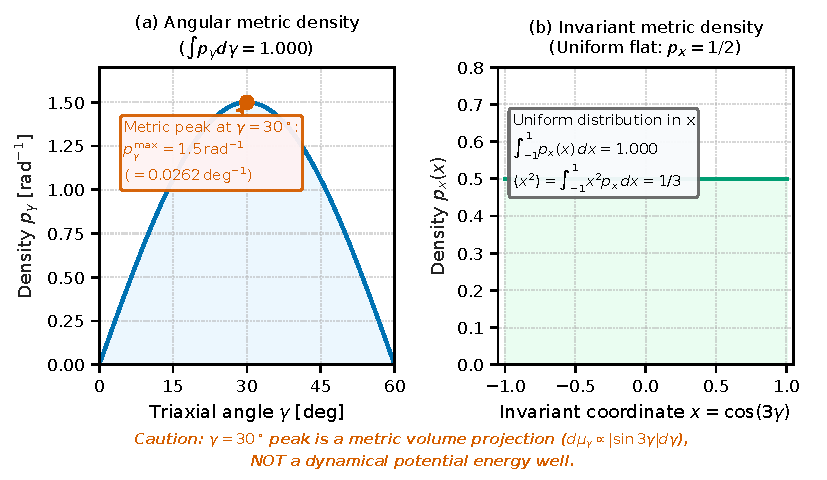
\includegraphics[width=0.85\textwidth]{Img/gamma-measure.pdf}
\caption{平坦角向势下不同坐标表象的概率密度与几何测度示意图。对于固定 $\beta$、自旋 $I=0$、常角向质量且 $\gamma$ 势平坦的受约束模型基态，在变量 $x=\cos 3\gamma \in [-1, 1]$ 下概率分布为平坦常数 $p_x(x)=1/2$，而在形状角 $\gamma \in [0, \pi/3]$ 下由于体积元测度因子 $\sin 3\gamma$ 呈现分布 $p_\gamma(\gamma)=\frac{3}{2}\sin 3\gamma$，并在 $\gamma=30^\circ$ 处取得极值，展示了同一量子态在不同坐标选择下的测度依赖表象。}
\label{fig:gamma-measure}
\end{figure}
}{}
%
}{%
    \section{形状坐标、测度与集体量子化 [未完成]}\label{sec:2-4}%
    \textit{本节尚未完成。}%
}

%-- Section 2.5: 内禀参考与对称性恢复
\setcounter{section}{4}%
\IfFileExists{Tex/Sections/sec-2-5.tex}{%
    \section{内禀参考与对称性恢复}\label{sec:2-5}

在第2.1节中，我们建立了严格的球张量代数与角动量耦合规则；在第2.4节中，引入了刻画四极集体形状的玻尔坐标 $(\beta, \gamma)$、体轴欧拉角 $\Omega = (\phi, \theta, \psi)$ 以及相应的黎曼体积元测度。在低能核物理研究中，微观相互作用哈密顿量由强相互作用与电磁相互作用主导，宇称不守恒的弱相互作用效应极其微弱，因而在原子核结构研究中通常将空间反演不变性（宇称守恒）与空间各向同性（连续转动守恒）作为基本近似框架。

在微观平均场近似（如形变 Hartree-Fock 或 Nilsson 势场）或唯象集体模型中，为了在有限基底中直观吸纳强四极变形与配对关联，通常引入随核整体转动的“内禀主轴参考系”。然而，所求得的形变单体参考态 $|\Phi\rangle$（例如形变 Slater 行列式或 HFB 准粒子真空态）破坏了三维空间连续转动不变性，在全空间中不再是总角动量平方 $\hat{\mathbf{J}}^2$ 与实验室 $z$ 轴分量 $\hat{J}_z$ 的共同本征态。需要强调的是，采用内禀坐标描述本身并不必然破坏转动对称性——例如包含全部取向角 $\Omega$ 积分的玻尔统合集体波函数 $\Psi_{IM}(\beta, \gamma, \Omega) = \sum_K \Phi_K(\beta, \gamma) \mathcal{D}^I_{MK}(\Omega)$ 完全具备严格的良自旋量子数 $I$ 与实验室磁量子数 $M$。此处被破缺的，仅仅是作为变分试探波包引入的微观单参考态 $|\Phi\rangle$。

为了将这种破缺对称性的微观参考波包与在束 $\gamma$ 谱学直接观测到的分立能级和电磁跃迁对账，投影技术（Projection After Variation, PAV 或 Variation After Projection, VAP）是从该参考态构造具有确定好自旋与宇称态矢的一条明确理论路线（与准粒子无规相位近似 QRPA、生成坐标法 GCM 等并列）。本节系统阐述该参考波包对称破缺与实验室定态之间的物理关系，构建含 $\hbar$ 量纲规范的三维角动量投影算符与非正交度规核，推导 Hill-Wheeler 广义本征方程及其能标规范不变性，并深入剖析线性幺正宇称投影与反幺正手征操作的本质差别，最后给出两个最短可计算阶梯实例。关于群论投影乘法规则、复非正交两态久期矩阵因式分解及度规截断算法的严格数学推导，读者可进一步参阅附录~\ref{app:projection}。

\subsection{微观破缺参考态与实验室定态的物理关系}\label{sec:2-5-1}

在孤立原子核中，全同核子相互作用哈密顿量 $\hat{H}$ 满足严格的角动量对易关系：
\begin{equation}\label{eq:2-5-H-J-commute}
[\hat{H}, \hat{\mathbf{J}}] = 0, \quad [\hat{H}, \hat{\mathbf{J}}^2] = 0.
\end{equation}
实验室系中的真实物理本征态必须具有确定的良量子数 $|I, M\rangle$。然而，微观自洽场求得的静态形变参考态 $|\Phi\rangle$ 具备非零四极形变（如 $\beta > 0, \gamma \ne 0$），在三维空间有限转动下发生改变：
\begin{equation}\label{eq:2-5-broken-state}
\hat{R}(\Omega) |\Phi\rangle \ne |\Phi\rangle, \quad \hat{\mathbf{J}}^2 |\Phi\rangle \ne \hbar^2 I(I+1) |\Phi\rangle.
\end{equation}
因此，$|\Phi\rangle$ 并非实验室参考系的物理定态，而是不同总自旋 $I$、实验室取向 $M$ 和内禀主轴投影 $K$ 的物理态的相干叠加包：
\begin{equation}\label{eq:2-5-superposition}
|\Phi\rangle = \sum_{I, M, K} c_{IMK} |\Psi_{IM; K}\rangle.
\end{equation}

在此明确两项关键的理论边界：
\begin{enumerate}
\item \textbf{模型内禀形变参数绝非实验室直接测量算符}：微观势能面或唯象模型中引入的内禀四极形变参数 $(\beta, \gamma)$，仅仅是表征内禀参考波包几何构型的内部变分参数。在实验室系中，实验谱学直接观测的是跃迁矩阵元、能级寿命 $\tau$ 与静电四极矩 $Q$。从实验室可观测量反演内禀形变必须经过明确的波函数重叠与转动态展开假设（详见第1.5节），不能把理论计算中的内禀极小参数等同于实验室定域算符测得值；
\item \textbf{对称破缺与恢复的理论定位}：在热力学极限下宏观体系可发生真正的自发对称破缺；而原子核是有限介观量子体系，连续对称性在实验室系中严格守恒。引入内禀变形参考态仅是以牺牲转动对称性为代价吸纳短程配对与长程多极关联的变分手段。通过投影算符从 $|\Phi\rangle$ 中提取确定自旋宇称的分量，是连通微观势阱结构与在束谱学定态的重要物理桥梁。
\end{enumerate}

\subsection{角动量投影算符、非正交重叠核与过完备性}\label{sec:2-5-2}

恢复连续空间转动对称性的数学工具是李群 $\mathrm{SO}(3)$ 上的群投影算符。设欧拉角 $\Omega = (\phi, \theta, \psi)$ 定义了空间旋转，具有物理量纲 $\hbar$ 的空间有限转动算符严格写作：
\begin{equation}\label{eq:2-5-rot-op}
\hat{R}(\Omega) = \exp(-i \phi \hat{J}_z / \hbar) \exp(-i \theta \hat{J}_y / \hbar) \exp(-i \psi \hat{J}_z / \hbar).
\end{equation}
利用 Wigner 不可约表示矩阵 $D^I_{MK}(\Omega)$ 的紧致正交完备性，定义三维角动量投影算符（Peierls-Yoccoz 算符）为~\cite{book-suhonen-from-nucleons-to-nucleus,book-raduta-coherent-states}：
\begin{equation}\label{eq:2-5-proj-op}
P^I_{MK} = \frac{2I+1}{8\pi^2} \int d\Omega \, D^{I*}_{MK}(\Omega) \hat{R}(\Omega),
\end{equation}
其中不变 Haar 测度归一化为 $\int d\Omega = \int_0^{2\pi} d\phi \int_0^\pi \sin\theta d\theta \int_0^{2\pi} d\psi = 8\pi^2$。固定核子数奇偶的原子核状态空间分别只包含整数自旋（偶 $A$ 核）或半整数自旋（奇 $A$ 核）；式中的 $8\pi^2$ 欧拉角积分对该固定表示类使用。整数类对应李群 $\mathrm{SO}(3)$；半整数类使用覆盖群 $\mathrm{SU}(2)$ 上的单值表示，固定类内 $D^* D$ 与 $D^* \hat{R}$ 乘积在群中心元素作用下两次变号相互抵消，因而在 $8\pi^2$ 欧拉角域内单值积分。式~\eqref{eq:2-5-proj-algebra} 的代数关系在各固定表示类内严格成立，不声称跨整数与半整数混合同时具有单值正交性。

算符 $P^I_{MK}$ 将内禀态 $|\Phi\rangle$ 中内禀轴分量为 $K$ 的部分，投影为实验室系具有确定自旋 $I$、外部分量为 $M$ 的物理态：
\begin{equation}\label{eq:2-5-projected-state}
|IM; K\rangle = P^I_{MK} |\Phi\rangle.
\end{equation}
投影算符满足如下结合代数规则（证明见附录~\ref{sec:appB-1}）：
\begin{equation}\label{eq:2-5-proj-algebra}
(P^I_{MK})^\dagger = P^I_{KM}, \quad P^I_{MK} P^{I'}_{M'K'} = \delta_{II'} \delta_{KM'} P^I_{MK'}.
\end{equation}
需向初学者澄清：并非所有双下标单元 $P^I_{MK}$ 均是各自独立的厄米正交投影算符。代数关系~\eqref{eq:2-5-proj-algebra} 严格表明：只有对角单元 $P^I_{MM}$ 才是标准的厄米幂等正交投影算符（满足 $(P^I_{MM})^\dagger = P^I_{MM} = (P^I_{MM})^2$）；对于一般的非对角单元 $M \ne K$，$P^I_{MK}$ 并不具备厄米性或幂等性，其实质是连接不同内禀取向分量 $K$ 到实验室分量 $M$ 的非厄米张量转移或阶梯算符。由全核哈密顿量的转动不变性 $[\hat{H}, \hat{R}(\Omega)] = 0$，立即可得：
\begin{equation}\label{eq:2-5-H-P-commute}
[\hat{H}, P^I_{MK}] = 0.
\end{equation}

对于同一个内禀波包 $|\Phi\rangle$，由不同 $K$ 投影生成的态矢在实验室系中并不正交。定义内积重叠度规（Norm kernel）为：
\begin{equation}\label{eq:2-5-norm-kernel}
N^I_{KK'} \equiv \langle IM; K | IM; K' \rangle = \langle \Phi | (P^I_{MK})^\dagger P^I_{MK'} | \Phi \rangle = \langle \Phi | P^I_{KK'} | \Phi \rangle.
\end{equation}
将式~\eqref{eq:2-5-proj-op} 代入，重叠核与哈密顿量核显式表示为内禀参考态在转动算符下的平均：
\begin{align}
N^I_{KK'} &= \frac{2I+1}{8\pi^2} \int d\Omega \, D^{I*}_{KK'}(\Omega) \langle \Phi | \hat{R}(\Omega) | \Phi \rangle, \label{eq:2-5-norm-integral} \\
H^I_{KK'} &\equiv \langle IM; K | \hat{H} | IM; K' \rangle = \frac{2I+1}{8\pi^2} \int d\Omega \, D^{I*}_{KK'}(\Omega) \langle \Phi | \hat{H} \hat{R}(\Omega) | \Phi \rangle. \label{eq:2-5-hamiltonian-kernel}
\end{align}

\textbf{过完备性与零模冗余说明}：在多体组态空间中，由不同 $K$ 生成的态矢集合 $\{ |IM; K\rangle \}_K$ 并不自动构成线性无关基。内禀态自身的离散对称性可使某些 $K$ 态的范数严格为零，这些精确零范数冗余必须剔除；而在连续三轴演化中，重叠矩阵 $N^I$ 的某些本征值可能数值上极为接近零。在数值实现中，引入有限截断阈值 $\epsilon_{\text{cut}}$ 属于有界子空间截断近似，截断后的体系只在保留的主有效子空间内与原问题等价，必须做收敛性与数值稳定性检查（详见附录~\ref{sec:appB-2}）。

\subsection{Hill-Wheeler 广义本征方程与能标规范不变性}\label{sec:2-5-3}

为了在所选具有好角动量量子数（good-$I$）的投影试探空间中，变分求取包含不同 $K$ 混合的近似能谱与波函数，将试探态构建为线性叠加：
\begin{equation}\label{eq:2-5-trial-state}
|\Psi^{IM}\rangle = \sum_K c_K |IM; K\rangle = \sum_K c_K P^I_{MK} |\Phi\rangle.
\end{equation}
应用 Ritz 变分原理，要求能量期望值对展开矢量 $\mathbf{c}$ 变分为驻值：
\begin{equation}\label{eq:2-5-variation}
\delta \frac{\langle \Psi^{IM} | \hat{H} | \Psi^{IM} \rangle}{\langle \Psi^{IM} | \Psi^{IM} \rangle} = 0 \iff \delta \left( \sum_{K, K'} c_K^* H^I_{KK'} c_{K'} - E \sum_{K, K'} c_K^* N^I_{KK'} c_{K'} \right) = 0.
\end{equation}
对任意独立微元 $\delta c_K^*$，直接导出非正交基下的 Hill-Wheeler 广义本征方程：
\begin{equation}\label{eq:2-5-hill-wheeler}
\sum_{K'} \left( H^I_{KK'} - E N^I_{KK'} \right) c_{K'} = 0 \iff H^I \mathbf{c} = E N^I \mathbf{c}.
\end{equation}
非零解存在的充要条件是广义久期行列式为零：$\det(H^I - E N^I) = 0$（在剔除度规严格零模并限制于度规严格正定 $N^I > 0$ 的线性独立物理子空间中使用）。
需要强调，角动量投影严格确保了非零态矢具有确定的总自旋与磁量子数 $I, M$；但在有限试探空间中通过 Ritz 变分求得的态矢，一般并非全微观哈密顿量 $\hat{H}$ 在全空间中的严格本征态，而是该受限投影子空间内的最佳变分近似。

\textbf{能量零点规范平移定理}：全哈密顿量加上任意标量常数平移 $\hat{H} \to \hat{H} + c \hat{\mathbf{1}}$（$c \in \mathbb{R}$）时，只改变参考能标零点，物理能量间距 $\Delta E$ 与量子态本质必须严格不变。根据核积分定义式~\eqref{eq:2-5-hamiltonian-kernel}：
\begin{equation}\label{eq:2-5-shift-kernel}
\langle \Phi | (\hat{H} + c \hat{\mathbf{1}}) P^I_{KK'} | \Phi \rangle = \langle \Phi | \hat{H} P^I_{KK'} | \Phi \rangle + c \langle \Phi | P^I_{KK'} | \Phi \rangle = H^I_{KK'} + c N^I_{KK'}.
\end{equation}
因此在非正交基矢下，哈密顿量矩阵的严格变换规则为：
\begin{equation}\label{eq:2-5-H-shift-matrix}
H^I \to H^I + c N^I.
\end{equation}
代入 Hill-Wheeler 方程：
\begin{equation}\label{eq:2-5-gauge-invariance}
(H^I + c N^I) \mathbf{c}' = E' N^I \mathbf{c}' \iff H^I \mathbf{c}' = (E' - c) N^I \mathbf{c}'.
\end{equation}
这保证了物理特征能谱统一平移 $E' = E + c$，且本征子空间严格保持不变。在非简并情形下波函数矢量保持 $\mathbf{c}' = \mathbf{c}$；在简并子空间中亦可选定完全相同的正交基。

反之，若在非正交基下因混淆基矢重叠而错误地执行对角平移 $H^I \to H^I + c \mathbf{1}$（$\mathbf{1}$ 为单位阵），设 $E'$ 为平移后的实际能量，久期方程变为 $\det(H^I + c \mathbf{1} - E' N^I) = 0$。若定义相对于平移量的能量 $\varepsilon \equiv E' - c$，方程则写作 $\det[H^I + c(\mathbf{1} - N^I) - \varepsilon N^I] = 0$。由于度规包含非对角元 $N^I_{KK'} \ne 0$，非对角扰动项 $c(\mathbf{1} - N^I)$ 在一般情况下会虚假改变能级相对间距，并可能引发非物理的态漂移或态混合。因此，“加能量常数必须 $H \to H + c N$，不能只改对角 $H$”是非正交量子力学中的基本定理。

\subsection{线性幺正宇称投影与反幺正手征对称性的本质差别}\label{sec:2-5-4}

在有限核分立对称性中，空间反演宇称 $\hat{\Pi}$ 与手征反转算符 $\mathcal{C} = \mathcal{T} R_y(\pi)$ 具有截然不同的代数本质。

\subsubsection{线性幺正宇称投影}\label{sec:2-5-4-1}

空间反演算符 $\hat{\Pi}$ 作用于空间坐标 $\mathbf{r} \to -\mathbf{r}$。在多体空间中，$\hat{\Pi}$ 是严格的线性幺正算符：
\begin{equation}\label{eq:2-5-parity-unitary}
\hat{\Pi}^2 = \hat{\mathbf{1}}, \quad \hat{\Pi}^\dagger = \hat{\Pi}^{-1} = \hat{\Pi}, \quad \hat{\Pi}(c_1 |\psi_1\rangle + c_2 |\psi_2\rangle) = c_1 \hat{\Pi}|\psi_1\rangle + c_2 \hat{\Pi}|\psi_2\rangle.
\end{equation}
对于具有反射不对称形变（如八极形变 $\beta_3 \ne 0$）的内禀参考态 $|\Phi_{\text{oct}}\rangle$，宇称发生破缺。定义线性宇称投影算符：
\begin{equation}\label{eq:2-5-parity-proj}
P^\pm \equiv \frac{\hat{\mathbf{1}} \pm \hat{\Pi}}{2}.
\end{equation}
由 $\hat{\Pi}^2 = \hat{\mathbf{1}}$ 易证其满足标准正交投影性质：
\begin{equation}\label{eq:2-5-parity-projector-properties}
(P^\pm)^\dagger = P^\pm, \quad (P^\pm)^2 = P^\pm, \quad P^+ P^- = P^- P^+ = 0, \quad P^+ + P^- = \hat{\mathbf{1}}.
\end{equation}
算符 $P^\pm$ 将任意物理态严格分解为正宇称（$\pi = +1$）与负宇称（$\pi = -1$）正交子空间，其本征值 $\pi = \pm 1$ 具有定相规范不变性。

\subsubsection{反幺正手征对称性与反线性不可投影性}\label{sec:2-5-4-2}

手征反转算符定义为时间反演与绕内禀参考轴转动的复合操作：
\begin{equation}\label{eq:2-5-chiral-op-def}
\mathcal{C} \equiv \mathcal{T} R_y(\pi) = \mathcal{T} \exp(-i\pi \hat{J}_y / \hbar).
\end{equation}
时间反演算符 $\mathcal{T}$ 包含复共轭操作 $K$，使得 $\mathcal{C}$ 具有反线性（anti-linear）特征：
\begin{equation}\label{eq:2-5-C-anti-linear}
\mathcal{C} \left( c_1 |\psi_1\rangle + c_2 |\psi_2\rangle \right) = c_1^* \mathcal{C}|\psi_1\rangle + c_2^* \mathcal{C}|\psi_2\rangle.
\end{equation}
尽管第3.5.2节严格证明了恒等式 $\mathcal{C}^2 = +1$ 对任意自旋均成立，但绝对不能照搬式~\eqref{eq:2-5-parity-proj} 构造形如 $(\hat{\mathbf{1}} \pm \mathcal{C}) / 2$ 的表达式：
\begin{equation}\label{eq:2-5-non-linear-failure}
\frac{\hat{\mathbf{1}} \pm \mathcal{C}}{2} (c |\psi\rangle) = \frac{1}{2} \left( c |\psi\rangle \pm c^* \mathcal{C}|\psi\rangle \right) \ne c \left( \frac{\hat{\mathbf{1}} \pm \mathcal{C}}{2} |\psi\rangle \right) \quad (\text{当 } \operatorname{Im}c \ne 0).
\end{equation}
该式表明 $(\hat{\mathbf{1}} \pm \mathcal{C})/2$ 对复标量乘法不封闭，无法在复希尔伯特空间中分解出正交子空间；且其特征相因子在全局重定相 $|\psi'\rangle = e^{i\phi}|\psi\rangle$ 下变为 $\lambda' = e^{-2i\phi}\lambda$，其符号不具备规范不变性。

因此，手征对称性的恢复绝不能通过线性算符投影完成。在具有反幺正对称性（$[\hat{H}, \mathcal{C}] = 0$ 且 $\hat{H}$ 厄米）的前提下，左手波包 $|L\rangle$ 与右手波包 $|R\rangle = \mathcal{C}|L\rangle$ 具备相等的对角期望值 $h \equiv \langle L|\hat{H}|L\rangle = \langle R|\hat{H}|R\rangle$。在有限势垒下，两态通过非对角隧穿矩阵元 $k = \langle L|\hat{H}|R\rangle$ 发生动力学隧穿，其物理态完全由非正交基矢集合 $\{|L\rangle, |R\rangle\}$ 上的 $2 \times 2$ 广义本征方程 $H \mathbf{c} = E N \mathbf{c}$ 确定。

\subsection{最短可计算阶梯实例：非正交双态模型与轴对称角动量恢复}\label{sec:2-5-5}

\subsubsection{阶梯一：非正交双态隧穿模型的严格手算}\label{sec:2-5-5-1}

设左右归一态矢存在非零实重叠积分 $S \in \mathbb{R}$（$|S| < 1$）：$\langle L|L\rangle = \langle R|R\rangle = 1, \langle L|R\rangle = S$。度规与哈密顿量矩阵为：
\begin{equation}\label{eq:2-5-ladder1-matrices}
N = \begin{pmatrix} 1 & S \\ S & 1 \end{pmatrix}, \quad H = \begin{pmatrix} h & k \\ k & h \end{pmatrix} \quad (h, k \in \mathbb{R}).
\end{equation}
广义久期方程 $\det(H - E N) = (h - E)^2 - (k - E S)^2 = 0$ 给出对称与反对称态的代数特征根：
\begin{equation}\label{eq:2-5-ladder1-energies}
E_s = \frac{h + k}{1 + S}, \quad E_a = \frac{h - k}{1 - S}.
\end{equation}
两根的相对代数差为 $E_a - E_s = \frac{2(h S - k)}{1 - S^2}$。按基矢对称/反对称分类，对称叠加态 $|\psi_s\rangle \propto (|L\rangle + |R\rangle)$ 对应能量 $E_s$，反对称叠加态 $|\psi_a\rangle \propto (|L\rangle - |R\rangle)$ 对应能量 $E_a$。在实轴上按能量从低到高排列：
\begin{equation}\label{eq:2-5-ladder1-ordered-energies}
E_{\text{low}} = \min(E_s, E_a), \quad E_{\text{high}} = \max(E_s, E_a).
\end{equation}
物理非负能级间距（能隙）恒由绝对值给出：
\begin{equation}\label{eq:2-5-ladder1-gap}
\Delta E_{\text{phys}} \equiv E_{\text{high}} - E_{\text{low}} = |E_a - E_s| = \frac{2|h S - k|}{1 - S^2}.
\end{equation}

显式验算规范不变性：
\begin{enumerate}
\item 若 $H \to H + c N$，则 $h' = h + c$，$k' = k + c S$。分子组合 $h' S - k' = (h + c) S - (k + c S) = h S - k$ 严格保持不变，能隙 $\Delta E_{\text{phys}}$ 独立于 $c$；
\item 若体系相互作用为纯单位阵 $\hat{H} = h \hat{\mathbf{1}}$，则 $H = h N \implies k = h S$，能隙 $\Delta E_{\text{phys}} = 0$ 严格为零。基矢几何重叠 $S \ne 0$ 本身绝不产生虚假能级分裂。
\end{enumerate}

\subsubsection{阶梯二：轴对称变形波包的投影与离散对称性选择定则}\label{sec:2-5-5-2}

设内禀波包 $|\Phi\rangle$ 具备绕内禀 $z$ 轴的连续轴对称性（主轴投影为 $K = 0$）：
\begin{equation}\label{eq:2-5-axial-condition}
\hat{J}_{z, \text{intr}} |\Phi\rangle = 0 \implies \hat{R}_{z, \text{intr}}(\psi) |\Phi\rangle = |\Phi\rangle.
\end{equation}
根据投影算符定义式~\eqref{eq:2-5-proj-op}，投影态矢为：
\begin{equation}\label{eq:2-5-axial-proj-state}
P^I_{M0} |\Phi\rangle = \frac{2I+1}{8\pi^2} \int_0^{2\pi} d\phi \int_0^\pi \sin\theta \, d\theta \int_0^{2\pi} d\psi \, D^{I*}_{M0}(\phi, \theta, \psi) \hat{R}(\phi, \theta, \psi) |\Phi\rangle.
\end{equation}
对于 $K = 0$，Wigner 函数化为：
\begin{equation}\label{eq:2-5-D-axial-form}
D^{I*}_{M0}(\phi, \theta, \psi) = d^I_{M0}(\theta) e^{i M \phi},
\end{equation}
对内禀角 $\psi$ 的积分直接给出因子 $2\pi$。态矢化简为：
\begin{equation}\label{eq:2-5-axial-state-simplified}
P^I_{M0} |\Phi\rangle = \frac{2I+1}{4\pi} \int_0^{2\pi} d\phi \, e^{i M \phi} e^{-i \phi \hat{J}_z / \hbar} \int_0^\pi \sin\theta \, d\theta \, d^I_{M0}(\theta) e^{-i \theta \hat{J}_y / \hbar} |\Phi\rangle.
\end{equation}
注意式中对实验室方位角 $\phi$ 的积分依然保留，它确保了态矢具有确切的实验室磁量子数 $M \in \{-I, -I+1, \dots, +I\}$。在各向同性空间中，全部 $2I+1$ 个 $M$ 态严格简并。

\textbf{离散旋转对称性与自旋选择定则}：空间反演宇称 $\hat{\Pi}$ 本身不能单独导出能带只含偶自旋 $I$。自旋限制来源于内禀波包在绕垂直主轴（内禀 $y$ 轴）旋转 $\pi$ 下的离散对称性（离散 $D_2$ 转动点群中绕垂直轴的 $\pi$ 转动对称性）：
\begin{equation}\label{eq:2-5-Ry-symmetry}
\hat{R}_{y, \text{intr}}(\pi) |\Phi\rangle = \exp(-i\pi \hat{J}_{y, \text{intr}} / \hbar) |\Phi\rangle = + |\Phi\rangle.
\end{equation}
将该对称操作作用于投影态矢，利用角动量算符结合规则：
\begin{equation}\label{eq:2-5-P-rot-commute}
P^I_{MK} \hat{R}(\Omega) = \sum_{K'} D^I_{K K'}(\Omega) P^I_{MK'}.
\end{equation}
由此展开得到：
\begin{align}\label{eq:2-5-spin-selection-derivation}
P^I_{M0} |\Phi\rangle &= P^I_{M0} \hat{R}_{y, \text{intr}}(\pi) |\Phi\rangle \nonumber \\
&= D^I_{00}(0, \pi, 0) P^I_{M0} |\Phi\rangle \nonumber \\
&= d^I_{00}(\pi) P^I_{M0} |\Phi\rangle.
\end{align}
由于 $d^I_{00}(\pi) = (-1)^I$，上式直接给出严格恒等式：
\begin{equation}\label{eq:2-5-even-spin-condition}
P^I_{M0} |\Phi\rangle = (-1)^I P^I_{M0} |\Phi\rangle.
\end{equation}
由此得出明确选择定则：当 $I$ 为奇数时，$P^I_{M0} |\Phi\rangle \equiv 0$ 恒等于零；非零投影态只能具有偶数自旋（$I = 0, 2, 4, \dots$）。偶 $I$ 投影态是否实际非零，还取决于内禀参考态中该自旋分量的展开权重（若波包中某偶 $I$ 振幅为零，则投影仍为零）。

在计算重叠度规核 $N^I_{00} \equiv \langle \Phi | P^I_{00} | \Phi \rangle$ 时，由于两端夹上轴对称态使得 $\phi$ 积分亦化简为 $2\pi$，度规核退化为一维转动重叠积分：
\begin{equation}\label{eq:2-5-axial-norm-integral}
N^I_{00} = \frac{2I+1}{2} \int_0^\pi \sin\theta \, d\theta \, d^I_{00}(\theta) \langle \Phi | \exp(-i \theta \hat{J}_y / \hbar) | \Phi \rangle.
\end{equation}
在单 $K$ 投影近似下，态能量为比值 $E(I) = H^I_{00} / N^I_{00}$。若额外引入强变形与绝热展开近似（即内禀态重叠函数 $\langle \Phi | e^{-i\theta \hat{J}_y/\hbar} | \Phi \rangle$ 随转角 $\theta$ 急剧衰减并允许转动能局域展开），该式可导出行如：
\begin{equation}\label{eq:2-5-rot-band-emergence}
E(I) \approx E_0 + \frac{\hbar^2}{2\mathcal{J}_{\text{eff}}} I(I+1)
\end{equation}
的转子能谱。然而，纯角动量投影本身不自动保证严格的刚体转子能谱；在实际核中，形变柔软度、科里奥利反配对效应与准粒子重排会导致能谱显著偏离理想转子。
%
}{%
    \section{内禀参考与对称性恢复 [未完成]}\label{sec:2-5}%
    \textit{本节尚未完成。}%
}

%-- Section 2.6: 势能、惯量与微观响应
\setcounter{section}{5}%
\IfFileExists{Tex/Sections/sec-2-6.tex}{%
    \section{势能、惯量与微观响应}\label{sec:2-6}

势能面标出不同约束构型的相对能量，却没有同时回答体系沿这些构型运动需要多大的动量。第2.3节的配对准粒子与第2.4节的集体坐标，恰好提供了补上这一环节的两端：前者决定哪些微观激发可以响应外场，后者规定如何用质量参数组织慢运动。因而，解释一个低能激发，既要问势能面是否容许这种偏离，也要问相应坐标如何响应扰动。较低的激发能、较大的沿带惯量和较宽的形状分布，不能只凭名称互相替代。

本节先用局部谐振问题明确单位和可辨识的参数组合，再从冻结准粒子场的响应进入自洽残余响应，最后比较配对规范转动、沿带转动和摆动的横向响应。除明确给出的局部教学推导外，微观公式均限定在相应来源实际采用的参考态与近似中。\cite{prochniak-rohozinski-2009-bohr-collective-hamiltonian,hinohara-2015-nambu-goldstone-inertia-response,matsuzaki-2004-nuclear-inertia-and-wobbling}

\subsection{从一个形状坐标的频率开始}\label{sec:2-6-1}

在一个稳定极小点附近，令形状偏离量为无量纲坐标 \(q\)，并在这一小邻域将其质量参数近似为正常数 \(B_q\)。去掉不影响激发能的常数项，最小的局部模型是
\begin{equation}\label{eq:2-6-local-hamiltonian}
H_{\mathrm{loc}}=\frac{p_q^2}{2B_q}+\frac{C_q}{2}q^2,
\qquad B_q>0,\quad C_q>0 .
\end{equation}
Hamilton方程给出 \(\dot q=p_q/B_q\) 与 \(\dot p_q=-C_q q\)，从而
\begin{equation}\label{eq:2-6-local-frequency}
\ddot q+\frac{C_q}{B_q}q=0,\qquad
\omega_q^2=\frac{C_q}{B_q},\qquad
\Delta E_q=\hbar\omega_q .
\end{equation}
这里 \(\omega_q\) 是角频率，\(\Delta E_q\) 是谐振相邻级间隔；不能把二者在恢复单位以后仍当作同一数值量。由于 \(q\) 无量纲，\(p_q\) 带作用量单位，故 \(B_q\) 的单位为 \(\hbar^2/\mathrm{MeV}\)，而 \(C_q\) 的单位为 \(\mathrm{MeV}\)。若写 \(B_q=\hbar^2 b_q\)，则
\begin{equation}\label{eq:2-6-local-energy-units}
[b_q]=\mathrm{MeV}^{-1},\qquad
\Delta E_q=\sqrt{\frac{C_q}{b_q}} .
\end{equation}
这几式是本稿在声明局部模型下的直接推导，并非某个实核的计算结果。

给出 \(C_q\) 尚不能确定 \(\Delta E_q\)：同一势曲率可与不同质量相配。反过来，只知道一个激发能也只限制 \(C_q/B_q\)，不能唯一决定曲率。即使进一步使用谐振基态的宽度
\begin{equation}\label{eq:2-6-local-width}
\langle q^2\rangle_0=\frac{\hbar}{2B_q\omega_q}
=\frac{\hbar}{2\sqrt{B_qC_q}},
\end{equation}
也须先证明所用电磁探针确实测到与这个 \(q\) 对应的算符及其尺度，才能把强度信息转成第二个约束。低能的 \(\gamma\) 候选态究竟来自较小曲率、较大质量，还是组态混合，因而需要能谱与算符信息共同判断。

这些关系仅适用于指定驻点附近的小振幅、局部常质量近似。若坐标改成有量纲的四极矩，质量与曲率都要随坐标变换；若出现大振幅混合、质量的明显坐标依赖或交叉动能项，便需处理相应集体Hamiltonian。进入该Hamiltonian的量子集体势也不自动等于未经零点修正的静态约束平均场能量。\cite[Secs.~3.1, 4.1--4.3]{prochniak-rohozinski-2009-bohr-collective-hamiltonian}

\subsection{质量参数由坐标和扰动共同定义}\label{sec:2-6-2}

对一组慢坐标 \(q^a\)，质量矩阵通过
\begin{equation}\label{eq:2-6-coordinate-mass}
T=\frac12\sum_{ab}M_{ab}(q)\dot q^a\dot q^b
\end{equation}
定义。保持同一个动能而改用坐标 \(Q^i\) 时，链式法则要求
\begin{equation}\label{eq:2-6-mass-transform}
M^{(Q)}_{ij}
=\sum_{ab}\frac{\partial q^a}{\partial Q^i}
M^{(q)}_{ab}
\frac{\partial q^b}{\partial Q^j}.
\end{equation}
因此，不同坐标约定中都标成“质量”的数值，须先转换到同一动能表达后才能比较。这个变换规律也说明：势能曲率与质量各自的数值会随坐标变化，物理频率不能仅由其中一个数值判断。

沿Próchniak与Rohoziński的 \(\beta,\gamma\) 约定，振动与空间转动的经典动能分别写成
\begin{equation}\label{eq:2-6-bohr-vibrational-mass}
\begin{aligned}
T_{\mathrm{vib}}=\frac12\bigl[
&B_{\beta\beta}\dot\beta^2
+2\beta B_{\beta\gamma}\dot\beta\dot\gamma\\
&+\beta^2 B_{\gamma\gamma}\dot\gamma^2\bigr],
\end{aligned}
\end{equation}
\begin{equation}\label{eq:2-6-bohr-rotational-mass}
T_{\mathrm{rot}}=\frac12\sum_{k=1}^3\mathcal J_k\omega_k^2,
\qquad
\mathcal J_k=4B_k\beta^2
\sin^2\!\left(\gamma-\frac{2\pi k}{3}\right).
\end{equation}
这里 \(\gamma\) 用弧度，轴标号须与所选主轴约定一致。式\eqref{eq:2-6-bohr-vibrational-mass}中，坐标质量矩阵的 \(\gamma\gamma\) 元是 \(\beta^2B_{\gamma\gamma}\)，而非单独的 \(B_{\gamma\gamma}\)；同样，\(B_k\) 也不是实际绕轴惯量 \(\mathcal J_k\) 本身。这是原综述Eqs.~(3.5)--(3.8)的动能约定，不能只看两个等高线图的色标单位就将它们等同。\cite[Eqs.~(3.5)--(3.8)]{prochniak-rohozinski-2009-bohr-collective-hamiltonian}

“惯量”还用于几种不同的响应。形状振动质量联系形状速度与共轭动量；空间转动惯量联系角速度与角动量；沿能带的运动学、动力学惯量来自同一转动序列的能量关系；配对转动惯量则联系化学势变化与平均粒子数变化。它们可受同一配对场影响，却不是同一算符或同一方向的响应。实验上由带内能差提取一个数值，并没有同时测定全部形状质量或横向响应张量。

\subsection{冻结场的Inglis--Belyaev响应}\label{sec:2-6-3}

在零温、偶偶时间反演不变的BCS型参考中，准粒子真空的低阶响应可先由两准粒子激发构造。沿上述综述Eq.~(4.44)的全单粒子空间求和约定，将角动量恢复为 \(\hat J_k=\hbar\hat j_k\)，转动惯量的Inglis--Belyaev（IB）式为
\begin{equation}\label{eq:2-6-ib-full-sum}
\mathcal J_k^{\mathrm{IB}}
=\hbar^2\sum_{\mu,\nu\ {\rm all}}
\frac{|\langle\nu|\hat j_k|\bar\mu\rangle|^2
(u_\mu v_\nu-u_\nu v_\mu)^2}
{E_\mu+E_\nu}.
\end{equation}
\(\bar\mu\) 表示与 \(\mu\) 对应的时间反演伙伴；\(u_\mu,v_\mu\) 是第2.3节中无量纲的占据振幅，\(E_\mu>0\) 是准粒子能量。这里的求和遍及完整选定单粒子基底，不能在这一式前再无条件添加一个来自“正负磁态”的因子2。\cite[PDF~p.~34, Eq.~(4.44)]{prochniak-rohozinski-2009-bohr-collective-hamiltonian}

另一种常用写法先把外场写成两准粒子产生、湮灭分量，并仅对不重复的 \(\mu<\nu\) 求和。若相应的无量纲角动量矩阵元为 \(j^{20}_{k,\mu\nu}\)，同一独立准粒子静态响应写为
\begin{equation}\label{eq:2-6-ib-pair-sum}
\frac{\mathcal J_k^{\mathrm{IB}}}{\hbar^2}
=2\sum_{\mu<\nu}
\frac{|j^{20}_{k,\mu\nu}|^2}{E_\mu+E_\nu}.
\end{equation}
式\eqref{eq:2-6-ib-full-sum}与式\eqref{eq:2-6-ib-pair-sum}采用不同的基底及对计数表示，转换须同时转换相干因子、时间反演相位和外场的 \(20\) 分量；不能只根据求和符号的外观判断是否少了一个2。附录\ref{app:C}给出本节使用的响应归一约定。

IB近似保留的是给定准粒子能量和给定外场矩阵元的响应，没有把扰动诱导的平均场变化重新反馈进来。综述在ATDHFB的Eqs.~(4.21)--(4.25)中明确指出，舍去Thouless--Valatin项后才出现这一简化；振动质量还要用到密度与配对张量对形状坐标的导数，并非把转动式中的 \(\hat j_k\) 任意换成一个四极算符就已经得到完整振动质量。\cite[Eqs.~(4.21)--(4.25), (4.44)]{prochniak-rohozinski-2009-bohr-collective-hamiltonian}

配对通过能量分母和相干因子改变这类响应，但实际比较还会伴随占据、参考态和场的重排。减弱配对可以增大某些计算中的转动惯量，却不保证得到精确的刚体值；无配对的独立粒子响应仍依赖壳结构、所选势与算符。在相同参考态上比较IB与含残余作用的响应，才可能辨认遗漏反馈的影响，不能将不同形状、不同配对输入的差值全归给某一种修正。\cite{petrik-kortelainen-2018-rotational-tv-inertia}

\subsection{自洽残余响应与零频NG惯量}\label{sec:2-6-4}

微小外场同时改变密度和平均场时，外场激起的两准粒子振幅与诱导场须联立求解。在Hinohara的有限振幅法（FAM）记号中，将原文自然单位下的频率变量显式改记为探测能量 \(z=\hbar\omega_{\mathrm{probe}}\)，方程为
\begin{equation}\label{eq:2-6-fam-induced-field}
\begin{aligned}
(E_\mu+E_\nu-z)X_{\mu\nu}(z)
+\delta H^{20}_{\mu\nu}(z)&=-F^{20}_{\mu\nu},\\
(E_\mu+E_\nu+z)Y_{\mu\nu}(z)
+\delta H^{02}_{\mu\nu}(z)&=-F^{02}_{\mu\nu}.
\end{aligned}
\end{equation}
这里 \(X,Y\) 是每单位微扰幅度的线性响应，\(\delta H^{20},\delta H^{02}\) 本身依赖这些振幅。去掉诱导场才回到独立准粒子响应；保留它们所表示的残余响应，是Thouless--Valatin（TV）惯量区别于冻结场IB的重要内容。\cite[APS~PDF~p.~3, Eqs.~(32)--(33)]{hinohara-2015-nambu-goldstone-inertia-response}

在一个连续对称性被平均场参考态破缺、且残余响应与同一理论处理一致的情形中，线性化方程还应包含相应的Nambu--Goldstone（NG）模。这个零频条件检验的是指定近似的对称性实现，不能仅由PES在某个形状方向较软便推得。原文在局部QRPA空间中用共轭算符归一
\begin{equation}\label{eq:2-6-ng-normalization}
\langle[\hat Q,\hat P]\rangle=i
\end{equation}
来固定NG惯量的尺度。此处暂采用 \(\hbar=1\) 的局部算符约定；对空间转动可取无量纲生成元 \(\hat P=\hat j_k\)，而对粒子数规范转动可取 \(\hat P=\hat N\)。\cite[APS~PDF~p.~3, Eqs.~(15), (18)--(23)]{hinohara-2015-nambu-goldstone-inertia-response}

特别地，只有当QRPA矩阵 \(A,B\) 为实矩阵时，才能按 \(P^{20}=r+i s\) 的实、虚分量写出
\begin{equation}\label{eq:2-6-tv-real-imag}
M_P=2\left[
r^T(A+B)^{-1}r+s^T(A-B)^{-1}s
\right].
\end{equation}
这里的 \(A,B\) 是两准粒子QRPA核，\(B\) 不是前述集体质量。式中的逆只在相应源矢量支撑的可逆子空间使用，不能对含NG零方向的全空间无条件求普通矩阵逆。实 \(P^{20}\) 涉及 \(A+B\)，纯虚 \(P^{20}\) 涉及 \(A-B\)；复参考态或时间反演破缺时，应回到完整响应方程，不能一概指定某一分块。\cite[APS~PDF~p.~3, Eqs.~(20)--(23)]{hinohara-2015-nambu-goldstone-inertia-response}

按原作 \(H+\eta F\) 的微扰符号定义强度函数，生成元的静态分支满足
\begin{equation}\label{eq:2-6-static-tv}
S(\hat P;0)=-M_P,\qquad
\mathcal J_k^{\mathrm{TV}}=\hbar^2M_{j_k}.
\end{equation}
于是，对减能外场 \(H-h\hat j_k\)、\(h=\hbar\omega_k\)，同一局部静态惯量满足
\begin{equation}\label{eq:2-6-tv-susceptibility}
\mathcal J_k^{\mathrm{TV}}
=\hbar^2\left.
\frac{\partial\langle\hat j_k\rangle}{\partial h}
\right|_{h=0}
=\left.
\frac{\partial\langle\hat J_k\rangle}{\partial\omega_k}
\right|_{\omega_k=0}.
\end{equation}
减能外场的正响应与上式强度函数的负号是同一约定的两种表达。原文Eq.~(52)还区分了NG生成元在零频与非零频处的响应；这里求的是静态分支，不能把任意有限频率表达直接外推到原点而略去NG归一。\cite[APS~PDF~p.~5, Eqs.~(49)--(53)]{hinohara-2015-nambu-goldstone-inertia-response}\cite[PDF~pp.~4--5, Eq.~(18)]{petrik-kortelainen-2018-rotational-tv-inertia}

实际计算中的零模位置、伪模分离和残余项完备程度，都需要检查。TV也不能被概括成所有核、所有坐标上固定倍数的IB增大：改变响应核与在同一个正定二次型中单纯释放一个冻结变量，是两种比较。相应实验问题是：同一套波函数与算符能否同时解释转动能标及有关电磁强度，而不是先把一个经验倍率当作独立的微观机制。

\subsection{配对转动不是形状振动质量}\label{sec:2-6-5}

对于破缺粒子数规范对称性的HFB参考态，局部配对转动响应可用
\begin{equation}\label{eq:2-6-pairing-response}
M_N=\left.
\frac{\partial\langle\hat N\rangle}{\partial\lambda}
\right|_{N_0},
\qquad [M_N]=\mathrm{MeV}^{-1}
\end{equation}
定义。粒子数无量纲，故这里不再引入一个空间转动的 \(\hbar^2\) 因子。在指定其它粒子数、选择平滑自洽态族且局部响应非奇异时，内部总能量的二阶展开为
\begin{equation}\label{eq:2-6-pairing-curvature}
\begin{aligned}
E(N)=E(N_0)&+\lambda_0\Delta N
+\frac{(\Delta N)^2}{2M_N}+\cdots,\\
\frac{\partial^2E}{\partial N^2}
&=M_N^{-1},\qquad \Delta N=N-N_0 .
\end{aligned}
\end{equation}
这是本稿用总能量 \(E\) 写出的局部曲率关系。若采用正束缚能 \(B_+=-E\)，便有
\begin{equation}\label{eq:2-6-positive-binding-sign}
M_N^{-1}
=-\frac{\partial^2B_+}{\partial N^2}.
\end{equation}
正束缚能的曲率不能在不换号的情况下代入总能量公式。\footnote{Hinohara原文Eq.~(66)将其 \(B\) 称为binding energy，而Fig.~4图注同时比较 \(-B_{\mathrm{exp}}\)。本节另行声明 \(B_+=-E\)，保留原作记号的这一解释边界，不把原式的字母 \(B\) 静默识别为本稿正束缚能，也不据此推断作者程序的错误。}\cite[APS~PDF~pp.~8--9, Eqs.~(66)--(67), Fig.~4]{hinohara-2015-nambu-goldstone-inertia-response}

配对转动描述规范方向上的粒子数响应，配对振动则涉及配对幅度变化；二者都不同于空间取向或 \(\gamma\) 形状坐标。离散核质量可以对局部曲率提供约束，但离散差分、连续HFB延拓与粒子数恢复后的结果并不自动相等。这里的局部 \(\hat Q,\hat N\) 共轭归一，也不是在完整有限粒子数Hilbert空间中建立全局自伴规范角的证明。若配对破缺参考不再存在，便须重新判断所讨论的NG模式，而不能只将同一惯量公式机械延伸过去。\cite{hinohara-2015-nambu-goldstone-inertia-response}

\subsection{沿带导数与摆动横向响应}\label{sec:2-6-6}

在绕 \(x\) 轴平稳转动的指定解支上，常定义
\begin{equation}\label{eq:2-6-band-inertias}
\mathcal J^{(1)}
=\frac{\langle\hat J_x\rangle}{\omega_{\mathrm{rot}}},
\qquad
\mathcal J^{(2)}
=\frac{d\langle\hat J_x\rangle}{d\omega_{\mathrm{rot}}}.
\end{equation}
这两个量都沿同一解支改变转速。若用 \(h=\hbar\omega_{\mathrm{rot}}\) 与 \(\hat j_x=\hat J_x/\hbar\) 表示，
\(\mathcal J^{(2)}=\hbar^2d\langle\hat j_x\rangle/dh\)。
在平滑、驻定且自洽的推转解支上，也可由Routhian \(E'(h)=\langle H-h\hat j_x\rangle\) 的曲率求得它。Kvasil与Nazmitdinov的Fig.~3将这种同方向导数与RPA的TV惯量对照，作为其平均场极小点与伪模分离的一致性检查；这种比较有共同的参考态、扰动方向和实现条件。\cite[PDF~p.~4, Fig.~3及相邻正文]{kvasil-2006-dy156-yb162-crpa-wobbling}

对已正确建立自旋序列、以 \(\Delta I=2\) 跃迁为主的平滑转动带，原文还采用带内相邻 \(\gamma\) 能量之差的估计
\begin{equation}\label{eq:2-6-band-finite-difference}
\mathcal J^{(2)}\simeq
\frac{4\hbar^2}
{E_\gamma(I+2\to I)-E_\gamma(I\to I-2)} .
\end{equation}
这是指定转动映射下的有限差分，跨越带交叉、混合或错配的序列时，其解释需另作检验。一个较大的带内 \(\mathcal J^{(2)}\)，只说明沿该序列的能量差变化，尚未给出转轴向 \(y,z\) 偏转时的回复响应。

Matsuzaki等在指定非轴形变的推转Nilsson加RPA实现中得到
\begin{equation}\label{eq:2-6-wobbling-response}
\omega_{\mathrm{wob}}^2
=\omega_{\mathrm{rot}}^2
\frac{
[\mathcal J_x-\mathcal J_y^{\mathrm{eff}}(\omega_{\mathrm{wob}})]
[\mathcal J_x-\mathcal J_z^{\mathrm{eff}}(\omega_{\mathrm{wob}})]
}{
\mathcal J_y^{\mathrm{eff}}(\omega_{\mathrm{wob}})
\mathcal J_z^{\mathrm{eff}}(\omega_{\mathrm{wob}})
},
\end{equation}
其中 \(\mathcal J_x=\langle J_x\rangle/\omega_{\mathrm{rot}}\)，而横向有效惯量须在待求模频率处评价，并带着给定转速、形变与准粒子输入。式的结构虽类似三轴转子，却是一个含响应函数的隐式根条件，不能将沿带 \(\mathcal J^{(2)}\) 直接填入两个横向位置。\cite[PDF~pp.~3--5, Eqs.~(8)--(12)]{matsuzaki-2004-nuclear-inertia-and-wobbling}

该式中的 \(\omega\) 均按角频率理解；在原式中出现 \(\hbar\omega_n\) 的准粒子激发能应与它区分。原文Eq.~(11)另含因子 \(\omega_n^2-\omega_{\mathrm{rot}}^2\)，分离旋转坐标系中的冗余转动根。因此，前述静止破缺参考上的NG零频条件，不能被不加变换地用来要求这一旋转框架中的伪模也在 \(\omega_n=0\)。

即使式\eqref{eq:2-6-wobbling-response}右端允许实根，还须检查相应态的集体性和电磁连接。作者也指出Nilsson势的速度依赖会使其 \(\mathcal J_x\) 偏大，且未给出横向量的对应修正；这限制了将其惯量比作为无条件定量结果的用法。\cite[PDF~p.~5, Eq.~(12)后讨论]{matsuzaki-2004-nuclear-inertia-and-wobbling}

Kvasil与Nazmitdinov的Dy、Yb例子还说明，相近的带弯曲现象在同一研究中可以分别涉及形状软模和中子对顺排；其带交叉附近的配对隙采用了明确的唯象处方。不能因为使用了“自洽”或“RPA”便省去这些输入，更不能将个别 \(\gamma\) 分支的演化推广为所有软核的同一个极限。\cite[PDF~pp.~3--4, Eq.~(6), Figs.~2--3]{kvasil-2006-dy156-yb162-crpa-wobbling}

由此，PES、带内能差、带间激发能与绝对电磁跃迁提供的是相互补充的约束。对摆动或形状模的具体判断，需要同一组声明的形状、配对、残余响应和算符共同给出可比较预言；单独一个势谷、一个带内惯量或配对减弱趋势，都不足以完成横向模式的识别。
%
}{%
    \section{势能、惯量与微观响应 [未完成]}\label{sec:2-6}%
    \textit{本节尚未完成。}%
}

%-- Section 2.7: 有效电磁与弱算符
\setcounter{section}{6}%
\IfFileExists{Tex/Sections/sec-2-7.tex}{%
    \section{有效电磁与弱算符}\label{sec:2-7}

在第2.1节中，我们建立了不可约球张量代数与 Wigner-Eckart 严格定理；在第2.2节与第2.3节中，分别推演了自洽平均场、单极驱动壳演化以及 BCS 准粒子基态的构建方案；在第2.4节至第2.6节中，进一步将微观组态与宏观集体坐标 $(\beta, \gamma)$、欧拉角三维对称性恢复及微观响应惯量联系起来。然而，不论是通过大尺度组态相互作用（LSSM）对角化，还是通过投影平均场或准粒子无规相位近似（QRPA）计算，多体理论直接获得的本征态矢通常局限于一个人为截断的有界模型空间（如价壳层空间 $P$）。而在束 $\gamma$ 谱学与放射性衰变实验所直接测量的，是物理定态之间跃迁的绝对衰变几率、激发态寿命、分支比以及多极强度 $B(E2)$、$B(M1)$ 与 $B(GT)$。

这便引出了本节需要回答的核心问题：\textbf{同一个微观多体波函数，为何需要配备与截断模型空间相容的有效电磁与弱跃迁算符？直接在截断价空间中使用自由核子的裸算符，会在何种层面上引入系统偏差？}

本节将从全多体 Hilbert 空间的 $P/Q$ 正交划分与幺正解耦表象出发，阐明有效哈密顿量与有效跃迁算符协同重整化的微观机制，并揭示单体截断近似下诱导多体算符的物理含义；进而系统推演电多极巨共振核芯极化诱导的 $E2$ 有效电荷及其对空间径向波函数与轨道的敏感依赖，澄清其在不同模型空间下的非单调行为；剖析介子交换流与核芯一阶自旋极化对磁偶极 $M1$ 轨道 $g_l$ 与自旋 $g_s$ 因子的微观重整化；随后在完备状态空间中给出 Gamow-Teller (GT) 算符与 Ikeda 差和定则 $S_- - S_+ = 3(N-Z)$ 的严密对易子代数推导，严格区分裸算符几何差和定则与实测衰变率中轴矢量耦合常数 $g_A^2$ 的物理定义，并指明价空间截断对完备闭合性的破坏机制；最后剖析 $g_A$ 淬灭的核多体组态混合与亚核子自由度双重根源，指明将淬灭因子作普适标量常数外推的物理边界与反例。关于实用跃迁率常数与多极混合比 $\delta(E2/M1)$ 符号相位的在束角分布反演约定，移交第5.7节与第5.9节；单 $j$ 壳层 Seniority 代数半满壳 $B(E2)$ 相消定理与 $K$ 异能态阻碍度移交第4.6节；$\beta$ 缓发粒子发射与衰变能窗网络移交第4.7节。

\subsection{Hilbert 空间截断、幺正解耦与有效算符自洽性}\label{sec:2-7-1}

在完全严格的非相对论 $A$ 核子量子多体问题中，原子核系统的物理状态定义在无限维的完全 Hilbert 空间 $\mathcal{H}$ 内。强相互作用本征方程为：
\begin{equation}\label{eq:2-7-full-schrodinger}
\hat{H} |\Psi_\alpha\rangle = E_\alpha |\Psi_\alpha\rangle,
\end{equation}
其中 $\hat{H} = \hat{T} + \hat{V}_{NN} + \hat{V}_{3N}$ 包含动能、两体强核力及必要的三体力。由于 $\mathcal{H}$ 的自由度随粒子数与单粒子基矢基底呈指数级增长，实际核结构模型必须将全空间正交分解为低能模型空间（Model Space，亦称价空间，投影算符为 $P$）与其正交补空间（Excluded Space，投影算符为 $Q$）：
\begin{equation}\label{eq:2-7-PQ-projectors}
\begin{aligned}
P &= \sum_{i \in P} |\phi_i\rangle \langle \phi_i|, \quad Q = \sum_{j \in Q} |\phi_j\rangle \langle \phi_j|, \\
P^2 &= P, \quad Q^2 = Q, \quad P + Q = \mathbf{1}, \quad PQ = QP = 0.
\end{aligned}
\end{equation}
模型空间 $P$ 通常由费米面附近的若干活跃单粒子轨道构成（例如 $sd$ 壳、$pf$ 壳或 $A\approx 130$ 区的 $50\text{--}82$ 质中子主壳），而深能隙下的满壳核芯与高激发连续谱自由度则被划入 $Q$ 空间。

在形式多体理论中，Feshbach 或 Bloch-Horowitz 投影通过能量依赖的有效哈密顿量 $\hat{H}_{\mathrm{eff}}(E) = P\hat{H}P + P\hat{H}Q(E - Q\hat{H}Q)^{-1}Q\hat{H}P$ 建立价空间方程。其模型态投影 $|\Phi_\alpha\rangle = P|\Psi_\alpha\rangle$ 相互之间一般不满足正交性，具有非平庸的度规矩阵 $N_{\alpha\beta} = \langle \Phi_\alpha | \Phi_\beta \rangle = \langle \Psi_\alpha | P | \Psi_\beta \rangle \ne \delta_{\alpha\beta}$。

现代多体物理（如李-铃木方法、大久保变换或介质相似重整化群 IMSRG）更普遍采用保范数的幺正解耦变换（Unitary Decoupling）框架~\cite{book-suhonen-from-nucleons-to-nucleus}。引入一个全局幺正变换算符 $\hat{U} = \exp(\hat{S})$，其中生成元满足反厄米性 $\hat{S}^\dagger = -\hat{S}$，算符满足：
\begin{equation}\label{eq:2-7-unitary-U}
\hat{U}^\dagger \hat{U} = \hat{U} \hat{U}^\dagger = \mathbf{1}.
\end{equation}
将全空间哈密顿量 $\hat{H}$ 与任意可观测物理跃迁算符 $\hat{\mathcal{O}}$ 作相容的幺正旋转：
\begin{equation}\label{eq:2-7-unitary-transform}
\hat{H}' = \hat{U}^\dagger \hat{H} \hat{U}, \quad \hat{\mathcal{O}}' = \hat{U}^\dagger \hat{\mathcal{O}} \hat{U}.
\end{equation}
要求变换算符 $\hat{U}$ 满足价空间解耦条件，即消去联系 $P$ 与 $Q$ 的非对角块哈密顿矩阵元：
\begin{equation}\label{eq:2-7-decoupling-condition}
Q \hat{H}' P = 0, \quad P \hat{H}' Q = 0.
\end{equation}
在此条件下，价空间 $P$ 成为变换后哈密顿量 $\hat{H}'$ 的不变子空间。在价空间内求解低能本征问题：
\begin{equation}\label{eq:2-7-Heff-model}
\hat{H}_{\mathrm{eff}} |\Phi_\alpha\rangle = E_\alpha |\Phi_\alpha\rangle, \quad \hat{H}_{\mathrm{eff}} \equiv P \hat{H}' P, \quad |\Phi_\alpha\rangle = P |\Phi_\alpha\rangle.
\end{equation}
全空间物理态 $|\Psi_\alpha\rangle$ 由 $|\Psi_\alpha\rangle = \hat{U} |\Phi_\alpha\rangle$ 给出，且由 $\hat{U}$ 的幺正性保证基底度规正交归一：$\langle \Phi_\alpha | \Phi_\beta \rangle = \langle \Psi_\alpha | \hat{U} \hat{U}^\dagger | \Psi_\beta \rangle = \delta_{\alpha\beta}$。

考虑两物理本征态之间的真跃迁矩阵元：
\begin{equation}\label{eq:2-7-true-matrix-element}
\langle \Psi_\alpha | \hat{\mathcal{O}} | \Psi_\beta \rangle = \langle \Phi_\alpha | \hat{U}^\dagger \hat{\mathcal{O}} \hat{U} | \Phi_\beta \rangle = \langle \Phi_\alpha | \hat{\mathcal{O}}' | \Phi_\beta \rangle.
\end{equation}
由于模型态波函数完全处于价空间 $P$ 内（$|\Phi_\alpha\rangle = P |\Phi_\alpha\rangle$），上式可表述为价空间有效算符矩阵元：
\begin{equation}\label{eq:2-7-Oeff-matrix-element}
\langle \Psi_\alpha | \hat{\mathcal{O}} | \Psi_\beta \rangle = \langle \Phi_\alpha | P \hat{\mathcal{O}}' P | \Phi_\beta \rangle \equiv \langle \Phi_\alpha | \hat{\mathcal{O}}_{\mathrm{eff}} | \Phi_\beta \rangle, \quad \hat{\mathcal{O}}_{\mathrm{eff}} = P \left( \hat{U}^\dagger \hat{\mathcal{O}} \hat{U} \right) P.
\end{equation}

式~\eqref{eq:2-7-Oeff-matrix-element} 呈现出两个重要推论：
\begin{enumerate}
\item \textbf{哈密顿量与跃迁算符重整化的协同性：}
使 $\hat{H}$ 解耦的同一个幺正变换算符 $\hat{U}$，原则上必须对称地施加于跃迁算符 $\hat{\mathcal{O}}$ 之上。若在模型空间求解有效哈密顿量 $\hat{H}_{\mathrm{eff}}$ 的本征态，却在计算跃迁矩阵元时直接使用自由核子的裸算符 $\hat{\mathcal{O}}_{\mathrm{bare}} = P \hat{\mathcal{O}} P$，相当于略去了变换算符 $\hat{U}$ 所携带的 $P\text{--}Q$ 空间关联修正。在守恒矢量流等受对称性保护的特殊跃迁中，裸算符可以是合理的精确近似；但在涉及强组态混合与介子交换流的通道中，直接使用裸算符属于需要显式评估其遗漏关联的单体截断近似。
\item \textbf{截断近似与诱导多体算符（Induced Many-Body Operators）：}
设初始物理算符 $\hat{\mathcal{O}} = \hat{\mathcal{O}}^{(1)}$ 为单体算符（例如单粒子电荷或自旋）。利用 Baker-Campbell-Hausdorff (BCH) 公式展开，旋转后的算符一般会产生高阶多体换位项：
\begin{equation}\label{eq:2-7-BCH-expansion}
\hat{\mathcal{O}}' = \hat{\mathcal{O}} + [\hat{\mathcal{O}}, \hat{S}] + \frac{1}{2!} [[\hat{\mathcal{O}}, \hat{S}], \hat{S}] + \dots = \hat{\mathcal{O}}^{(1)}_{\mathrm{eff}} + \hat{\mathcal{O}}^{(2)}_{\mathrm{eff}} + \hat{\mathcal{O}}^{(3)}_{\mathrm{eff}} + \dots.
\end{equation}
在传统壳模型实践中，计算通常局限于单体算符框架（$\hat{\mathcal{O}}_{\mathrm{eff}} \approx \hat{\mathcal{O}}^{(1)}_{\mathrm{eff}}$），将诱导的多体效应平均吸收为单体基矢下的有效电荷与淬灭因子。
\end{enumerate}

\subsection{电多极跃迁、核芯极化与 E2 有效电荷}\label{sec:2-7-2}

在低能核结构谱学中，电四极跃迁 $E2$ 是揭示原子核集体形变与转动-振动行为的核心探针。在长波长、点状核子近似下，裸电多极算符定义为不可约球张量：
\begin{equation}\label{eq:2-7-bare-E-op}
\hat{\mathcal{M}}(E\lambda, \mu) = \sum_{i=1}^A e_i r_i^\lambda Y_{\lambda\mu}(\hat{\mathbf{r}}_i),
\end{equation}
其中核子坐标 $\mathbf{r}_i$ 相对原子核质心定义（在严格计算中需扣除质心假运动），在点核子表象下自由质子取裸电荷 $e_p = 1e$，自由中子取裸电荷 $e_n = 0e$（该设定在长波长电磁相互作用点核子近似下使用，不涉及有限分辨率下中子内禀电荷分布）。根据第2.1节已建立的统一 Wigner-Eckart 定理相位规范~\cite{book-suhonen-from-nucleons-to-nucleus}：
\begin{equation}\label{eq:2-7-wigner-eckart-phase}
\langle j_f m_f | T_{\lambda\mu} | j_i m_i \rangle = (-1)^{2\lambda} \frac{C_{j_i m_i \lambda\mu}^{j_f m_f}}{\sqrt{2j_f + 1}} \langle j_f || T_\lambda || j_i \rangle,
\end{equation}
对于整数多极度 $\lambda$，$(-1)^{2\lambda} \equiv 1$。从初态 $|I_i\rangle$ 向末态 $|I_f\rangle$ 的电磁辐射下行跃迁的约化跃迁几率 $B(E\lambda)$ 严格定义为：
\begin{equation}\label{eq:2-7-BE2-def}
B(E\lambda; I_i \to I_f) = \frac{1}{2I_i + 1} |\langle I_f || \hat{\mathcal{M}}(E\lambda) || I_i \rangle|^2.
\end{equation}
库仑激发中从基态向上跃迁的逆过程，由统计权重因子联系：
\begin{equation}\label{eq:2-7-up-down-relation}
\begin{aligned}
B(E\lambda; I_f \to I_i) &= \frac{2I_i + 1}{2I_f + 1} B(E\lambda; I_i \to I_f), \\
\text{例如 } B(E2; 0^+_{\mathrm{gs}} \to 2^+_1) &= 5 B(E2; 2^+_1 \to 0^+_{\mathrm{gs}}).
\end{aligned}
\end{equation}

在辐射场量子理论中，电多极跃迁发射率 $T(E\lambda)$ 在国际单位制（SI）下表达为：
\begin{equation}\label{eq:2-7-TE-rate-si}
T(E\lambda) = \frac{2}{\varepsilon_0 \hbar} \frac{\lambda + 1}{\lambda [(2\lambda + 1)!!]^2} \left(\frac{E_\gamma}{\hbar c}\right)^{2\lambda + 1} B(E\lambda).
\end{equation}
式~\eqref{eq:2-7-TE-rate-si} 中前置因子含真空介电常数 $1/(4\pi\varepsilon_0)$，采用高斯单位制时该系数对应转换为 $4\pi$。正如第5.9节中所严格核验与统一的实用数值公式，利用精细结构常数 $\alpha = e^2/(4\pi\varepsilon_0 \hbar c) \approx 1/137.04$ 与 $\hbar c \approx 197.33\,\mathrm{MeV}\cdot\mathrm{fm}$，将物理常数完全吸收后，电四极发射跃迁几率写作实用标准式~\cite{book-suhonen-from-nucleons-to-nucleus}：
\begin{equation}\label{eq:2-7-TE2-practical}
T(E2) = C_{E2} [E_\gamma(\mathrm{MeV})]^5 B(E2), \quad C_{E2} \approx 1.2250 \times 10^9 \quad [\mathrm{s}^{-1}\,\mathrm{MeV}^{-5}\,(e^2\,\mathrm{fm}^4)^{-1}].
\end{equation}
当 $B(E2)$ 采用微观单位 $e^2\,\mathrm{fm}^4$ 时，代入上式直接给出以 $\mathrm{s}^{-1}$ 为单位的衰变几率；若改用宏观单位 $e^2\,\mathrm{b}^2$（注意 $1\,\mathrm{b}^2 = 10^4\,\mathrm{fm}^4$，故数值上 $B(E2)(e^2\mathrm{fm}^4) = 10^4 B(E2)(e^2\mathrm{b}^2)$），相应的速率系数转换为 $C_{E2} \approx 1.2250 \times 10^{13}\,\mathrm{s}^{-1}\mathrm{MeV}^{-5}(e^2\mathrm{b}^2)^{-1}$。有关由激发态实验平均寿命 $\tau$、光子分支比 $b_k$ 与内转换系数反演提取绝对 $B(E2)$ 的完整测量模型，统一对齐至第5.9节。

若在模型空间 $P$ 中直接采用中子裸电荷 $e_n = 0$，则任何闭壳外单中子核素（例如 $^{209}\mathrm{Pb}$ 的中子单粒子跃迁）的预言电四极跃迁几率均恒等于零。然而实验上在单中子核中测得了明确的有限 $E2$ 跃迁，其强度常可达单粒子 Weisskopf 单位量级。

这一物理现象的微观本质是核芯极化（Core Polarization）~\cite{book-bohr-mottelson-nuclear-structure}。价核子（无论是质子还是中子）通过长程同位旋标量与同位旋矢量四极残余核力，与满壳核芯发生粒子-空穴耦合，在核芯中感应出虚的四极电荷形变，微观上对应于将核芯质子虚激发至高能巨四极共振态（Giant Quadrupole Resonance, GQR，等标激发能 $E_{\mathrm{ISGQR}} \approx 64 A^{-1/3}\text{ MeV}$，等矢激发能 $E_{\mathrm{IVGQR}} \approx 130 A^{-1/3}\text{ MeV}$）。

因此，在截断价空间中，单体算符吸收核芯极化后，核子获得单体有效电荷：
\begin{equation}\label{eq:2-7-eff-charge-def}
e_i^{\mathrm{eff}} = e_i^{\mathrm{bare}} + \delta e_i, \quad e_p^{\mathrm{eff}} = 1e + \delta e_p, \quad e_n^{\mathrm{eff}} = 0e + \delta e_n.
\end{equation}
极化电荷 $\delta e$ 在同位旋空间分解为等标（IS）与等矢（IV）两部分：
\begin{equation}\label{eq:2-7-isospin-pol-charge}
\delta e_i = \delta e^{(0)} + \tau_{3i} \delta e^{(1)}, \quad \tau_3 = \begin{cases} -1 & (\text{质子}) \\ +1 & (\text{中子}) \end{cases},
\end{equation}
使得 $\delta e_p = \delta e^{(0)} - \delta e^{(1)}$，$\delta e_n = \delta e^{(0)} + \delta e^{(1)}$。由于质中核力在标量道表现为强吸引，中子在核芯周围感应出质子核芯极化，导致常用经验参数中中子获得可观的有效电荷 $\delta e_n \approx 0.5e$，质子有效电荷则相应增强（在常见壳模型如 $sd$ 壳或 $A\approx 130$ 区空间中，常用经验参数为 $e_p^{\mathrm{eff}} \approx 1.5e\text{--}1.7e, e_n^{\mathrm{eff}} \approx 0.5e\text{--}0.7e$ 作为特定价空间的有效例）~\cite{book-nuclear-shell-model-70-years}。

有效电荷的大小由价核子径向波函数与核芯粒子-空穴对的微观极化积分决定，并不存在“模型空间变大有效电荷普遍单调减小”的简单法则：
\begin{enumerate}
\item \textbf{空间径向波函数与弱束缚边界：} 极化电荷具有空间重叠敏感性。当原子核趋近中子滴线或处于低束缚能单粒子轨道时，价核子波函数向核外弥散（如晕态或低轨道角动量 $s, p$ 态），与紧致核芯质子云的空间重叠减少，极化电荷 $\delta e$ 因而受到压低。
\item \textbf{单粒子轨道依赖性：} 不同的轨道 $(n, l, j)$ 具有不同的节点特征与空间局域性，其耦合核芯振动声子的微观矩阵元存在轨道差异。
\item \textbf{模型空间扩大与非单调反馈：} 虽然从单粒子截断走向无截断从头算极限时，核芯激发自由度最终被显式包含而恢复裸电荷；但在实际壳模型截断下，由单主壳层扩充至包含特定跨壳侵入轨道时，新引入的轨道间相互作用或形变驱动力可能改变基态组态混合比，进而局部改变某些通道的有效电荷需求。因此，有效电荷对模型空间的依赖由微观核芯激发自由度的划分边界决定，需结合具体相互作用核验。
\end{enumerate}

\subsection{磁多极跃迁、有效 g 因子与介子交换流}\label{sec:2-7-3}

磁多极跃迁算符探测的是原子核内的微观电流与自旋磁矩分布。自由核子的裸磁偶极算符写作：
\begin{equation}\label{eq:2-7-M1-bare}
\hat{\mathcal{M}}(M1, \mu) = \sqrt{\frac{3}{4\pi}} \mu_N \sum_{i=1}^A \left[ g_l^{\mathrm{bare}}(i) \hat{\mathbf{l}}_i + g_s^{\mathrm{bare}}(i) \hat{\mathbf{s}}_i \right]_\mu,
\end{equation}
其中 $\mu_N = \frac{e\hbar}{2 m_p}$ 为国际单位制（SI）下的核磁子（量纲为 $\mathrm{J}\cdot\mathrm{T}^{-1}$ 或 $\mathrm{A}\cdot\mathrm{m}^2$），角动量算符 $\hat{\mathbf{l}}$ 与 $\hat{\mathbf{s}}$ 均已无量纲化（已除以 $\hbar$）。自由核子的裸磁回旋比（$g$ 因子）精确测定值为：
\begin{equation}\label{eq:2-7-free-gfactors}
g_l^p = 1, \quad g_l^n = 0, \quad g_s^p \approx +5.5857, \quad g_s^n \approx -3.8261.
\end{equation}
磁偶极约化跃迁几率 $B(M1)$ 的单位为 $\mu_N^2$：
\begin{equation}\label{eq:2-7-BM1-def}
B(M1; I_i \to I_f) = \frac{1}{2I_i + 1} |\langle I_f || \hat{\mathcal{M}}(M1) || I_i \rangle|^2.
\end{equation}
统一对齐至第5.9节的换算体系，磁偶极辐射衰变跃迁几率实用式为：
\begin{equation}\label{eq:2-7-TM1-rate}
\begin{aligned}
T(M1) &= C_{M1} [E_\gamma(\mathrm{MeV})]^3 B(M1)(\mu_N^2), \\
C_{M1} &\approx 1.758 \times 10^{13} \quad [\mathrm{s}^{-1}\,\mathrm{MeV}^{-3}\,(\mu_N^2)^{-1}].
\end{aligned}
\end{equation}

在介质重整化过程中，自旋磁因子 $g_s$ 在核内核子中通常发生淬灭，而轨道磁因子 $g_l$ 则出现微小的等矢位移。其微观物理机制源于两种物理过程~\cite{book-suhonen-from-nucleons-to-nucleus,book-bohr-mottelson-nuclear-structure}：
\begin{enumerate}
\item \textbf{介子交换流（MEC）驱动的轨道 $g_l$ 修正：} 强核力由虚介子交换传递。带电 $\pi$ 介子在质子与中子之间跃迁时产生空间跨核子对流，这一非单体电磁流无法简单归结为单点核子的轨道环流，相当于在有效单粒子磁矩中引入等矢修正项。在双闭壳核附近的特定模型空间中，常用经验参数表示为：
\begin{equation}\label{eq:2-7-delta-gl}
g_l^{\mathrm{eff}} = g_l^{\mathrm{bare}} + \delta g_l, \quad \delta g_l \approx -0.10 \tau_3, \quad \text{即 } g_l^{p,\mathrm{eff}} \approx 1.10, \quad g_l^{n,\mathrm{eff}} \approx -0.10.
\end{equation}
需强调，式~\eqref{eq:2-7-delta-gl} 中的数值属于特定单粒子空间的有效唯象参数，反映了介子流引起的等矢重整化趋势，不代表全核区普适恒定的常数。
\item \textbf{一阶核芯自旋极化驱动的自旋 $g_s$ 淬灭：} 考虑自旋-轨道劈裂的单粒子轨道（$j_> = l + 1/2$ 与 $j_< = l - 1/2$）。价核子通过自旋-同位旋残余相互作用 $\hat{V}_{\sigma\tau} \sim \boldsymbol{\sigma}_1 \cdot \boldsymbol{\sigma}_2 \, \boldsymbol{\tau}_1 \cdot \boldsymbol{\tau}_2$ 激发核芯核子发生自旋翻转跃迁（$j_> \to j_<$），形成巨磁偶极共振（Giant $M1$ Resonance，激发能通常在 $8\text{--}10\text{ MeV}$）。这种 $1^+$ 粒子-空穴相干激发在价核子处感应出反向极化，削弱了自旋磁矩，导致有效自旋 $g$ 因子呈现淬灭：
\begin{equation}\label{eq:2-7-gs-quench}
g_s^{\mathrm{eff}} \approx (0.7\text{--}0.8) \, g_s^{\mathrm{bare}}.
\end{equation}
此外，高阶张量力重整化还在有效磁算符中诱导出一个二阶张量复合算符：
\begin{equation*}
g_p [\mathbf{Y}_2 \times \hat{\mathbf{s}}]_1 ,
\end{equation*}
体现了原子核内自旋磁化与空间四极形状的各向异性耦合。
\end{enumerate}

对于角动量和宇称均允许的同一条跃迁，$E2$ 与 $M1$ 辐射可以相干混合。相应的无量纲辐射振幅比记为 $\delta$。第5.7节和第5.9节分别讨论相位、角关联与偏振反演，以及辐射率和单位约定。

\subsection{Gamow-Teller 算符与 Ikeda 差和定则的严格推导}\label{sec:2-7-4}

弱相互作用 $\beta$ 衰变是连接同量异位素核态的关键探针。在无轨道角动量转移（$\Delta L = 0$）的允许跃迁中，微观单体衰变算符包含 Fermi 算符与 Gamow-Teller (GT) 算符：
\begin{equation}\label{eq:2-7-weak-operators}
\hat{\mathcal{O}}(F) = \sum_{k=1}^A t_\pm(k), \quad \hat{\mathcal{O}}(GT, \mu) = \sum_{k=1}^A \sigma_\mu(k) t_\pm(k),
\end{equation}
其中同位旋阶梯算符遵循核物理标准同位旋约定：
\begin{equation}\label{eq:2-7-isospin-ladder-convention}
\begin{aligned}
t_3 |n\rangle &= +\frac{1}{2} |n\rangle, \quad t_3 |p\rangle = -\frac{1}{2} |p\rangle; \\
t_- |n\rangle &= |p\rangle \quad (\beta^-\text{ 衰变}), \quad t_+ |p\rangle = |n\rangle \quad (\beta^+\text{/EC 衰变}).
\end{aligned}
\end{equation}
单核子同位旋对易关系为：
\begin{equation}\label{eq:2-7-isospin-commutator}
[t_+(k), t_-(k')] = \delta_{kk'} 2 t_3(k).
\end{equation}

在球张量表象下，定义 $\beta^\mp$ 衰变方向的裸 Gamow-Teller 跃迁算符为：
\begin{equation}\label{eq:2-7-beta-GT-pm}
\hat{\beta}^-_{GT}(\mu) = \sum_{k=1}^A \sigma_\mu(k) t_-(k), \quad \hat{\beta}^+_{GT}(\mu) = \sum_{k=1}^A \sigma_\mu(k) t_+(k).
\end{equation}
其厄米共轭算符具有相因子转换：
\begin{equation}\label{eq:2-7-hermitian-conjugate}
[\hat{\beta}^-_{GT}(\mu)]^\dagger = \sum_{k=1}^A \sigma_\mu^\dagger(k) t_-^\dagger(k) = (-1)^\mu \sum_{k=1}^A \sigma_{-\mu}(k) t_+(k) = (-1)^\mu \hat{\beta}^+_{GT}(-\mu).
\end{equation}
定义总 Gamow-Teller 跃迁强度为对所有可能可达末态 $|f_\mp\rangle$ 的约化跃迁几率求和：
\begin{equation}\label{eq:2-7-sum-definitions}
S_- = \sum_{f_-} B(GT^-; 0^+_i \to 1^+_{f_-}), \quad S_+ = \sum_{f_+} B(GT^+; 0^+_i \to 1^+_{f_+}),
\end{equation}
其中单态间的 $B(GT)$ 按标准无因次算符矩阵元定义（\textbf{不包含耦合常数 $g_A^2$}）：
\begin{equation}\label{eq:2-7-BGT-bare-def}
B(GT^\mp; 0^+_i \to 1^+_{f_\mp}) = \sum_{M_f \mu} |\langle 1^+_{f_\mp} M_f | \hat{\beta}^\mp_{GT}(\mu) | 0^+_i \rangle|^2 = |\langle 1^+_{f_\mp} || \hat{\boldsymbol{\sigma}} t_\mp || 0^+_i \rangle|^2.
\end{equation}

现在我们在完全 Hilbert 空间中推导著名的 \textbf{Ikeda 差和定则（Ikeda Sum Rule）}~\cite{book-suhonen-from-nucleons-to-nucleus}。将 $S_-$ 展开，并利用完全末态空间的完备性闭合条件 $\sum_{f_-} |f_-\rangle \langle f_-| = \mathbf{1}$：
\begin{align}\label{eq:2-7-Sminus-derivation}
S_- &= \sum_{f_-} \sum_\mu \langle 0^+_i | [\hat{\beta}^-_{GT}(\mu)]^\dagger | f_-\rangle \langle f_- | \hat{\beta}^-_{GT}(\mu) | 0^+_i \rangle \nonumber\\
&= \sum_\mu (-1)^\mu \langle 0^+_i | \hat{\beta}^+_{GT}(-\mu) \left( \sum_{f_-} |f_-\rangle \langle f_-| \right) \hat{\beta}^-_{GT}(\mu) | 0^+_i \rangle \nonumber\\
&= \sum_\mu (-1)^\mu \langle 0^+_i | \hat{\beta}^+_{GT}(-\mu) \hat{\beta}^-_{GT}(\mu) | 0^+_i \rangle.
\end{align}
同理，对 $S_+$ 做相同的展开并变换求和角标 $\mu \to -\mu$，得到：
\begin{equation}\label{eq:2-7-Splus-derivation}
S_+ = \sum_\mu (-1)^\mu \langle 0^+_i | \hat{\beta}^-_{GT}(\mu) \hat{\beta}^+_{GT}(-\mu) | 0^+_i \rangle.
\end{equation}
两者相减，强度差直接转化为基态对易子的期望值：
\begin{equation}\label{eq:2-7-diff-commutator}
S_- - S_+ = \sum_\mu (-1)^\mu \langle 0^+_i | \left[ \hat{\beta}^+_{GT}(-\mu), \hat{\beta}^-_{GT}(\mu) \right] | 0^+_i \rangle.
\end{equation}
将微观坐标算符代入对易子：
\begin{align}\label{eq:2-7-commutator-eval}
\left[ \hat{\beta}^+_{GT}(-\mu), \hat{\beta}^-_{GT}(\mu) \right] &= \sum_{k, k'=1}^A \left[ \sigma_{-\mu}(k) t_+(k), \sigma_\mu(k') t_-(k') \right] \nonumber\\
&= \sum_{k=1}^A \left\{ \sigma_{-\mu}(k) \sigma_\mu(k) t_+(k) t_-(k) - \sigma_\mu(k) \sigma_{-\mu}(k) t_-(k) t_+(k) \right\},
\end{align}
其中不同核子标号 $k \ne k'$ 的对易子严格为零。利用 Pauli 算符在同一核子上的代数性质，球分量求和满足收缩关系：
\begin{equation}\label{eq:2-7-pauli-contraction}
\sum_{\mu=-1}^1 (-1)^\mu \sigma_{-\mu}(k) \sigma_\mu(k) = \hat{\boldsymbol{\sigma}}(k) \cdot \hat{\boldsymbol{\sigma}}(k) = \sigma_x^2 + \sigma_y^2 + \sigma_z^2 = 3 \cdot \mathbf{1}_2.
\end{equation}
同时，由于同位旋对易子为标量，对 $\mu$ 求和后 Pauli 矩阵的反向项具有完全相同的缩并值 3。因此对易子对 $\mu$ 的加权和化简为：
\begin{align}\label{eq:2-7-commutator-final}
\sum_{\mu=-1}^1 (-1)^\mu \left[ \hat{\beta}^+_{GT}(-\mu), \hat{\beta}^-_{GT}(\mu) \right] &= \sum_{k=1}^A 3 \left( t_+(k) t_-(k) - t_-(k) t_+(k) \right) \nonumber\\
&= 3 \sum_{k=1}^A [t_+(k), t_-(k)] = 3 \sum_{k=1}^A 2 t_3(k) \\
&= 6 \sum_{k=1}^A t_3(k) = 6 \hat{T}_3.
\end{align}
原子核基态的总同位旋第三分量由中子数与质子数唯一确定：
\begin{equation*}
\langle 0^+_i | \hat{T}_3 | 0^+_i \rangle = \frac{1}{2}(N - Z) .
\end{equation*}
代入式~\eqref{eq:2-7-commutator-final}，得到完全不依赖于波函数相互作用细节的 \textbf{Ikeda 和定则}：
\begin{equation}\label{eq:2-7-ikeda-result}
S_- - S_+ = 6 \cdot \frac{N - Z}{2} = 3(N - Z).
\end{equation}
这一推导清晰地指出了系数 3 的物理根源：它来自三维空间 Pauli 自旋算符的标量平方和 $\hat{\boldsymbol{\sigma}}^2 = \sigma_x^2 + \sigma_y^2 + \sigma_z^2 = 3 \cdot \mathbf{1}_2$，既非“未配对中子数”，也非简单中子自旋投影态计数。

在此需要澄清两个关键物理边界：
\begin{enumerate}
\item \textbf{算符代数和定则与实测衰变速率的严格解耦：}
式~\eqref{eq:2-7-ikeda-result} 是无量纲单体算符在完备空间中的纯空间-同位旋几何代数恒等式，\textbf{其定义本身完全不包含轴矢量耦合常数 $g_A$}。在真实实验中，实测放射性衰变速率（或比较半衰期 $ft$ 值）包含弱相互作用拉氏量的耦合常数与轻子相空间积分 $f_0$：
\begin{equation}\label{eq:2-7-ft-value}
f_0 t_{1/2} = \frac{\kappa}{g_V^2 B(F) + g_A^2 B(GT)}, \quad \kappa = \frac{2\pi^3 \hbar^7 \ln 2}{m_e^5 c^4 G_F^2 |V_{ud}|^2} \approx 6147\text{ s}.
\end{equation}
若某些文献在定义跃迁几率时将耦合常数预先乘入（即令 $\widetilde{B}(GT) \equiv g_A^2 B(GT)$），则相应的强度差和必须同步带上该因子：$\widetilde{S}_- - \widetilde{S}_+ = 3 g_A^2 (N-Z)$。两者在概念定义上必须明确分开。
\item \textbf{模型截断破坏闭合性与差和的非对称遗漏：}
式~\eqref{eq:2-7-Sminus-derivation} 的数学基础是中间态求和在全 Hilbert 空间完备：$\sum_f |f\rangle \langle f| = \mathbf{1}$。然而在任何截断模型空间 $P$ 中，中间态求和仅限于有限个价空间基矢：$\sum_{f \in P} |f\rangle \langle f| = P \ne \mathbf{1}$。完备性被截断破坏。更重要的是，Ikeda 和定则是两个正通道 $S_-$ 与 $S_+$ 的差值。在模型空间截断下，$S_-$ 缺失了位于高能巨共振及高能连续谱的强度，而 $S_+$ 同样丢失了可能存在的未占据空穴激发通道强度。因此，截断空间中的强度差值 $\sum_{f_- \in P} B(GT^-) - \sum_{f_+ \in P} B(GT^+)$ 不保证满足 $3(N-Z)$，且在不同核素与截断方案下不具有单向必然偏小的简单单调性质。
\end{enumerate}

\subsection{轴矢量耦合常数淬灭的多源性与非普适性}\label{sec:2-7-5}

通过电荷交换反应（如 $(p, n)$ 与 $(^3\mathrm{He}, t)$）在零度散射角下对原子核 Gamow-Teller 强度分布的测量表明，在低能离散态乃至局部巨共振能量窗口内，实测的 $\sum B(GT^-) - \sum B(GT^+)$ 强度通常低于自由单体 Ikeda 差和定则预言值 $3(N-Z)$。在传统大尺度壳模型等若干指定价空间的经验例中，为了复现实验低能离散跃迁的 $\log ft$ 值，通常需要引入一个有效淬灭因子 $q_A \approx 0.70\text{--}0.77$（即采用 $g_A^{\mathrm{eff}} = q_A g_A^{\mathrm{free}}$；例如 Gysbers 等在文献~\cite{gysbers-2019-ab-initio-beta-decay-quenching} 图 1 中所对比的传统模型唯象参考值 $q_A \approx 0.75$）作为特定模型空间与能窗下的有效参数。

现代微观多体物理表明，强度在低能窗的不饱和不能归咎于单一物理机制，而是包含两类物理机制的共同贡献：
\begin{enumerate}
\item \textbf{核多体组态混合：} 核力中的非中心张量力与其他短程残余核力诱发核子间发生强烈的粒子-空穴激发（如高能 $2p\text{--}2h$ 组态），将相当一部分 Gamow-Teller 跃迁强度搬运至几十兆电子伏特的高激发能连续谱区域，超出了低能衰变乃至局部峰区测量的实验积分窗口。
\item \textbf{介子交换与强子自由度：} 在核介质环境中，带电介子流的存在以及核子被虚激发为自旋-同位旋共振态（如 $\Delta_{33}(1232\text{ MeV})$ 共振态），产生弱两体电流（Two-Body Currents, 2BC），在单粒子轴矢量算符矩阵元中引入负相干贡献。
\end{enumerate}

近年基于手征有效场论的微观多体研究进一步考察了淬灭机制。Gysbers 等采用手征核力 Hamiltonian 结合从头算耦合簇（CC）与价空间 IMSRG 方法，研究轻核至 $^{100}\mathrm{Sn}$ 的 Gamow-Teller 衰变~\cite{gysbers-2019-ab-initio-beta-decay-quenching}；Wang 等则在双闭壳核（$^{56}\mathrm{Ni}$、$^{100}\mathrm{Sn}$、$^{132}\mathrm{Sn}$）中，基于 Skyrme 能量密度泛函（如 SGII、SkM* 等）采用 RPA 结合粒子-振动耦合（RPA+PVC）并计入手征弱两体流~\cite{wang-2026-axial-coupling-quenching-joint-effects}。多体波函数关联与弱两体流应在指定框架下配套处理。Gysbers 等的比较还表明，先加入关联或先加入两体流，会改变对淬灭“主要来源”的分配；这种归因依赖相互作用的分辨率与比较路径，不能提炼为跨模型固定的主次顺序。各计算框架还具有各自的截断、低能常数拟合输入与理论不确定度，不同模型之间的数值结果不能直接相加。

更重要的是，\textbf{在科学论证上不能将低能唯象的 $q_A \approx 0.75$ 当作一个无条件的普适常数跨核区、跨过程随意套用}。这一边界具有明确的物理考量：
\begin{itemize}
\item \textbf{一阶禁戒（First-Forbidden, FF）弱衰变中的算符与动量非普适性：}
在远离稳定线的中子丰富核区（如超新星 $r$-过程快中子俘获等待点核 $^{130}\mathrm{Cd}$ 或 $^{78}\mathrm{Ni}$ 邻区），一阶禁戒跃迁贡献了相当大甚至主导的衰变宽度。一禁戒算符包含不同张量秩与空间对称性的多个独立算符（例如秩为 0 的类时轴荷算符 $\gamma_5$；秩为 1 的空间矢量流 $\mathbf{r}$、$\boldsymbol{\alpha}$ 与 $\boldsymbol{\sigma}\times\mathbf{r}$；秩为 2 的张量算符 $[\boldsymbol{\sigma} \times \mathbf{r}]_2$）。Zhi 等人在特定价空间与有效相互作用下的微观计算表明~\cite{doctoral-r1-g34-zhi-2013-prc-shell-model-half-lives}：由于软 $\pi$ 介子交换流在核介质中的特殊相干机制，一阶禁戒衰变中的类时轴荷算符表现出介质增强效应（拟合有效参数 $q_A > 1$），而空间流算符则呈现出不同程度的淬灭。尽管具体的有效拟合系数取决于所选用的价空间与相互作用模型，该结果明确表明弱衰变算符具有本质的秩与动量依赖性，不能将单一标量淬灭因子外推至所有禁戒通道。
\item \textbf{无中微子双贝塔衰变（$0\nu\beta\beta$）的不同动量与多极权重：}
通常的允许单 $\beta$ 跃迁采用外部动量转移 $q_{\mathrm{ext}}R/\hbar\ll1$ 的长波近似，相应多体波函数仍保留核内的费米运动。轻中微子交换机制下的 $0\nu\beta\beta$ 则涉及核子间的虚中微子传播，典型内部交换动量约为 $|\mathbf q_\nu|\sim100\text{--}200\,\mathrm{MeV}/c$，相应核矩阵元具有不同的动量和多极权重~\cite{engel-menendez-2017-double-beta-matrix-elements-review}。常用率公式可以外提 $g_A^4$，但核矩阵元及有效算符本身仍须在所用约定下一致处理。因此，低能单 $\beta$ 衰变拟合的淬灭因子不能直接移植到 $0\nu\beta\beta$ 中换算寿命。
\end{itemize}

\subsection{本节小结与后续章节接口}\label{sec:2-7-6}

本节确立了连接微观模型波函数与实际在束谱学及衰变实验可观测量的算符一致性基础。主要物理结论与边界总结如下：
\begin{enumerate}
\item \textbf{模型截断与有效算符对偶：} 在所声明的幺正解耦构造中，有效哈密顿量与有效算符由同一变换得到，计算时应保持二者的截断精度相容。变换一般会诱导多体算符；有效电荷或淬灭因子只是把部分贡献压缩到单体形式的一种近似，具体方法是否需要这种参数化应另行判断。
\item \textbf{电四极极化微观图像：} 在常用价空间中，经验参数 $e_p^{\mathrm{eff}} \approx 1.5e, e_n^{\mathrm{eff}} \approx 0.5e$ 反映了价核子与核芯巨四极共振粒子-空穴对的相干极化；有效电荷受单粒子径向波函数空间重叠与具体模型空间划分调制，不表现为机械的单调函数。
\item \textbf{磁偶极双重机制：} 轨道磁矩 $g_l$ 在特定空间中通过荷电介子交换流获得微小等矢修正（$\delta g_l \approx -0.10\tau_3$）；自旋磁矩 $g_s$ 则由于一阶核芯自旋-轨道巨 $M1$ 共振激发而呈现淬灭（$g_s^{\mathrm{eff}} \approx (0.7\text{--}0.8) g_s^{\mathrm{bare}}$）。
\item \textbf{Ikeda 和定则与完备性：} 裸 Gamow-Teller 算符在完备空间中的差和定则为 $S_- - S_+ = 3(N-Z)$，系数 3 来自 Pauli 自旋算符的标量平方和 $\hat{\boldsymbol{\sigma}}^2 = 3 \cdot \mathbf{1}_2$。此处的裸算符定义不含衰变率中的 $g_A^2$ 因子。截断中间态求和后，能否保留该差和取决于所保留空间与算符是否仍闭合相应代数；有限价空间并不自动违反、也不自动保证完整差和。
\item \textbf{淬灭多源性与过程依赖：} 对低能跃迁拟合的 $g_A^{\mathrm{eff}}$ 同时反映所用多体波函数、被消去的空间及保留的弱流算符。组态关联与两体流的贡献应在指定实现中配套评估。一禁戒跃迁的不同秩算符可需要不同修正，其中类时轴荷存在增强的实例；这不等于所有禁戒算符具有同一增强因子。$0\nu\beta\beta$ 涉及不同的动量与多极权重，其弱流和核矩阵元修正须另行计算，不能直接移用低能单 $\beta$ 衰变拟合的单一因子。
\end{enumerate}

本节所确立的算符规范，为后续各章构筑了清晰的理论接口：
\begin{itemize}
\item \textbf{对第3章（三轴集体激发模式判定）：} 第3.2节（摆动运动横向与纵向分支）中带间 $E2_{\mathrm{out}}$ 与带内 $E2_{\mathrm{in}}$ 强度比、第3.5节（手征双重带对称性破缺）中特征 $B(M1)/B(E2)$ 锯齿交错选择定则，均严格建立在本节给出的多极有效电荷与有效 $g$ 因子框架之上。
\item \textbf{对第4章（六区前沿比较与两翼探针）：} 第4.6节中单 $j$ 壳层 Seniority 代数半满壳 $B(E2)$ 严格相消证明，将承袭本节的有效单粒子矩阵元规范；第4.7节关于 $r$-过程快中子俘获等待点核的 $\beta$ 衰变与缓发中子发射概率，将直接应用本节确立的 Gamow-Teller 与一禁戒非普适淬灭理论。
\item \textbf{对第5章（在束实验谱学技术链）：} 第5.7节关于方向角关联（DCO）与偏振测量反演多极混合比 $\delta(E2/M1)$、第5.9节关于由激发态绝对平均寿命 $\tau$、光子分支比与内转换系数提取绝对约化跃迁几率 $B(E2)$ 与 $B(M1)$ 的精确数值换算，将在本节量纲与初末态统计权定义下完全闭合。
\end{itemize}
%
}{%
    \section{有效电磁与弱算符 [未完成]}\label{sec:2-7}%
    \textit{本节尚未完成。}%
}

%-- Section 2.8: 模型各自保留和消去了什么
\setcounter{section}{7}%
\IfFileExists{Tex/Sections/sec-2-8.tex}{%
    \section{模型各自保留和消去了什么}\label{sec:2-8}

原子核是一个强相互作用有限量子多体系统。直接求解包含核子间基本微观核力的全空间薛定谔方程，在微观上受限于指数增加的基矢维度，在宏观上难以直观展现体系在低激发能区呈现出的相干集体运动。为此，核结构理论发展出了涵盖微观组态展开、自洽能量密度泛函、代数玻色子映射、绝热集体哈密顿量与推转转子模型的理论谱系。在实际研究中，若简单地将模型划分为“全微观”与“唯象”，或仅凭模型能对个别低激发能级给出符合曲线便断言运动模式已确立，往往会掩盖不同物理图像背后的自由度假设与局限性。

第\ref{chap:2}章前七节从实验室张量对称性（第\ref{sec:2-1}节）、单极相互作用驱动的壳演化（第\ref{sec:2-2}节）、准粒子配对与相变（第\ref{sec:2-3}节）、玻尔形状坐标与测度（第\ref{sec:2-4}节）、对称性恢复投影（第\ref{sec:2-5}节）、微观动能响应与惯量张量（第\ref{sec:2-6}节）以及有效电磁与弱算符重整化（第\ref{sec:2-7}节），建立了从核子微观运动到集体量子形状的描述基础。作为本章的总结，本节对主流核结构模型展开比较分析：明确各模型保留了哪些活跃自由度、消去或冻结了哪些动力学过程；分析不同模型对同一套实验能级展现拟合简并的物理原因；确立在模型比较中适用的认识论界限；并结合具体的实验测量案例与六质量区的特征，讨论如何借助留出检验（holdout validation）与独立高阶观测量约束模型，为后续讨论三轴非轴对称转动与高阶耦合动力学提供参照。\cite{bohr-mottelson-1953-collective-individual-original,book-bohr-mottelson-nuclear-structure-vol2,prochniak-rohozinski-2009-bohr-collective-hamiltonian,poves-2020-limits-assigning-nuclear-shape}

\subsection{有效自由度的分离与希尔伯特空间的截断尺度}\label{sec:2-8-1}

在低能核物理中，理论模型通常是对全多体希尔伯特空间在特定能标和截断尺度下的有效映射。在低能核多体问题中，常规的微观近似起点通常写为包含单体动能、两体相互作用与三体相互作用的非相对论形式：
\begin{equation}\label{eq:2-8-bare-hamiltonian}
\hat{H} = \sum_{i} \hat{t}_i + \sum_{i<j} \hat{v}_{ij} + \sum_{i<j<k} \hat{v}_{ijk} .
\end{equation}
式\eqref{eq:2-8-bare-hamiltonian}略去了更高阶的多体相互作用，且质心运动（Center-of-Mass, CM）的分离与修正须按具体微观模型进行专门处理。在微观计算中，其组态维度随核子数和价空间急剧增加；若采用基于自由核子散射的传统唯象核力，须处理短程排斥效应，而若采用现代手征有效场论核力配合相似重整化群（SRG）软化演化，单粒子势矩阵元虽更为平滑，但会诱导产生多体有效力。

物理上，原子核表现出特征能标的分离：核子内部自由度激发的能标处于数百 $\mathrm{MeV}$ 以上；核芯单核子跨主壳激发的能标在 $\hbar\omega_0 \approx 41 A^{-1/3}\,\mathrm{MeV}$ 量级（数至十数 $\mathrm{MeV}$）；表面四极振动与准粒子拆对的能标在 $1\sim 2\,\mathrm{MeV}$；而中重形变核的集体转动激发能标则通常低于数百 $\mathrm{keV}$。这种特征能标的层级，决定了不同物理问题需要选取相适应的模型空间。

保留哪些变量、怎样处理其余动力学，是比较模型的一条共同线索；但不同理论不必都是同一个微观哈密顿量的字面投影。对已经给定哈密顿量的Hilbert空间问题，可以用正交投影 $\hat P,\hat Q$ 分出模型空间与其补空间。Feshbach--Bloch--Horowitz构造给出一种能量依赖的有效哈密顿量：
\begin{equation}\label{eq:2-8-feshbach-projection}
\hat{H}_{\mathrm{eff}}(E) = \hat{P}\hat{H}\hat{P} + \hat{P}\hat{H}\hat{Q}\frac{1}{E - \hat{Q}\hat{H}\hat{Q}}\hat{Q}\hat{H}\hat{P} .
\end{equation}
这里式\eqref{eq:2-8-feshbach-projection}是一个特定的能量依赖构造，其有效定义要求能量 $E$ 处于 $Q$ 空间预解式 $(E - \hat{Q}\hat{H}\hat{Q})^{-1}$ 存在的非奇异能量区间。需要指出，并非所有有效哈密顿量都必须依赖能量，例如第\ref{sec:2-7}节提及的通过正则幺正变换、Lee--Suzuki 相似变换或 SRG 演化构建的模型空间有效哈密顿量，可以在模型空间内消除能量依赖性。相应物理观测量算符 $\hat{\mathcal{O}}$ 在投影空间中的有效算符 $\hat{\mathcal{O}}_{\mathrm{eff}}$，其重整化修正不仅包含微观核芯极化贡献，还包含多体有效算符项与非正交基底变换诱导的度规修正（如第\ref{sec:2-7}节所讨论），不能简化为单一的核芯极化项。这一构造显示了被消去动力学如何反馈到模型空间。对其它理论，也应检查保留变量、参数与算符的一致性，但不能默认存在同一套字面的投影映射。

\subsection{八类主流核结构模型的物理透视}\label{sec:2-8-2}

为了给后续章节关于三轴形变、手征进动与取向耦合激发模式的讨论提供系统参照，本小节梳理低能核结构领域中八类代表性模型体系在自由度保留、动力学截断、参数来源及适用区域上的特征。\cite{book-bohr-mottelson-nuclear-structure-vol2,book-suhonen-from-nucleons-to-nucleus,prochniak-rohozinski-2009-bohr-collective-hamiltonian,frauendorf-2001-spontaneous-symmetry-breaking-rotating-nuclei,doctoral-r1-g28-otsuka-2023-type-ii-shell-evolution}

\paragraph{1. 大规模微观壳模型 (Shell Model / CI / MCSM)}
大规模壳模型以球形单粒子平均场单核子轨道为基底，在选定的单或多价壳层空间内建立完全反对称的多费米子组态空间。
\begin{itemize}
\item \textbf{保留的自由度}：价轨道上每个核子的独立产生与湮灭算符 $a^\dagger_j, a_j$；自旋-轨道耦合与两体单极、多极残余相互作用；多粒子-多空穴激发的微观相干叠加。
\item \textbf{消去的动力学}：冻结深束缚的惰性核芯（inert core）；截断价空间以外的高能虚激发与连续谱耦合；核芯极化效应被吸收到价空间两体有效相互作用矩阵元（TBME）中。
\item \textbf{参数来源}：可从微观核力及重整化出发，也可用选定谱学资料拟合价空间相互作用；具体计算常结合两种信息。USD、GXPF1、JUN45及 $V_{\mathrm{MU}}$ 等作用各有构造与标定范围，不能默认它们都是同一路线的无参数推导。\cite{doctoral-r1-g28-otsuka-2023-type-ii-shell-evolution}
\item \textbf{主要输出与观测联系}：实验室好角动量与好宇称下的能级 $E(I^\pi)$、单核子谱因子 $S_j$、电磁约化跃迁几率 $B(E2)$ 和 $B(M1)$、核电四极矩 $Q(I)$ 与磁偶极矩 $\mu(I)$；结合求和规则可计算核形状不变量。
\item \textbf{典型失效边界}：随着价核子数和价轨道数增加，组态矩阵维度呈指数增加，在中重变形区计算受限；当跨壳粒子-空穴侵入态与正常组态强混合时，单一固定价空间截断失效。
\end{itemize}

\paragraph{2. 自洽平均场与能量密度泛函 (Self-Consistent Mean Field / EDF / HFB / CDFT)}
自洽能量密度泛函理论将多体基态能量表述为单体局域密度、动能密度、自旋-轨道密度及反常配对张量的泛函。
\begin{itemize}
\item \textbf{保留的自由度}：选定单参考态的单体密度、配对场及对约束外场的响应；泛函可含局域或非局域结构。实际计算也有基底与数值截断。
\item \textbf{消去的动力学}：单个参考态本身不包含不同形状构型间的大振幅量子叠加。参考态可以按求解条件破缺转动、粒子数或空间反演等对称性，并非每个解都破缺全部对称性；恢复与混合需另行处理。
\item \textbf{参数来源}：全局拟合核素图的基本性质（结合能、电荷半径、核物质饱和密度、不可压缩模 $K_0$、对称能及其斜率参数 $L$，如Skyrme SLy4、Gogny D1S/D1M、相对论微观泛函PC-PK1/DD-PC1）。
\item \textbf{主要输出与观测联系}：结合能、电荷半径、约束势面及极小处的形变。自洽单粒子谱与第2.2节定义的ESPE或实验谱重心不是自动相同的量。
\item \textbf{典型失效边界}：单参考态的一个极小不能独自表示软势面的量子涨落，也不能直接给出全部具有好量子数的激发谱与跃迁率。一般经验EDF不自动对应一个反对称多体算符，非对角核与高阶修正需逐实现定义；基于明确多体算符的构造则应保留其自身条件。
\end{itemize}

\paragraph{3. 五维玻尔集体哈密顿量 (5DCH / Bohr Collective Hamiltonian 基于自洽微观输入)}
五维玻尔集体哈密顿量在大振幅四极形变空间与空间转动欧拉角空间建立绝热动力学方程。\cite{prochniak-rohozinski-2009-bohr-collective-hamiltonian}
\begin{itemize}
\item \textbf{保留的自由度}：内禀四极形变标量坐标 $(\beta, \gamma)$ 与描述空间取向的三个欧拉角 $\Omega = (\phi, \theta, \psi)$ 共五个集体坐标。
\item \textbf{消去的动力学}：绝热近似下消去了非平衡单粒子跃迁与内禀准粒子激发的解对动力学；冻结了除四极外的更高极自由度；忽略了转动下科里奥利力引起的准粒子非绝热顺排。
\item \textbf{参数来源}：在相应微观映射中，使用约束HFB/EDF的势面、零点能处方、振动质量张量与转动惯量。质量与逆质量应按第2.6节约定区分；IB、完整TV及各类cranking近似也不能仅因同名而互换。
\item \textbf{主要输出与观测联系}：偶偶核低激发正宇称态能谱（基态带、$\gamma$ 振动带、$\beta$ 振动带）、态波函数在形变平面的概率分布 $|\Psi_I(\beta, \gamma)|^2$、绝对跃迁几率 $B(E2)$ 与跃迁四极矩。
\item \textbf{典型失效边界}：无法直接描述高自旋下单核子高 $j$ 轨道顺排引起的带回弯（backbending）与高 $K$ 异能态费米子阻塞；在配对相变临界点（$\Delta \to 0$）或基态能级交叉处，微观 IB 质量张量出现奇异性，绝热分离假设受限。
\end{itemize}

\paragraph{4. 投影生成坐标法 (Projected GCM / PGCM / SCC-GCM)}
投影生成坐标法通过对破缺对称性的形变多体波函数连续流形进行相干叠加，并通过投影算符恢复实验室守恒对称性。\cite{heyde-wood-2011-shape-coexistence-review,prochniak-rohozinski-2009-bohr-collective-hamiltonian}
\begin{itemize}
\item \textbf{保留的自由度}：在选定的生成坐标空间（如四极形变 $\beta, \gamma$ 及对能隙 $\Delta$）构成的内禀态流形 $\{|\Phi(q)\rangle\}$ 上构建连续相干量子叠加；通过投影算符 $\hat{P}^N, \allowbreak \hat{P}^Z, \allowbreak \hat{P}^I_{MK}, \allowbreak \hat{P}^\pi$ 保留实验室守恒量子数。
\item \textbf{消去的动力学}：受限于选定的有限生成坐标集合 $\{q\}$，消去了未纳入该坐标流形的正交微观空间动力学自由度；变分后投影（PAV）忽略了转动态对内禀基底的反作用。
\item \textbf{参数来源}：由微观有效核相互作用或自洽能量泛函决定，无须唯象假定集体动能质量张量。
\item \textbf{主要输出与观测联系}：好量子数 $(I^\pi, N, Z)$ 下的态能谱、形状共存构型的混合权重、形状跃迁矩阵元、电荷半径同位素移动。
\item \textbf{典型失效边界}：在包含非对角过渡密度的多参考经验泛函实现中需注意自相互作用与正则化检验；同时高自旋三维欧拉角投影数值积分计算量大。
\end{itemize}

\paragraph{5. 相互作用玻色子模型 (Interacting Boson Model / IBM / IBFM)}
相互作用玻色子模型将价核子对映射为具有低角动量的单极与四极玻色子系统。\cite{book-casten-nuclear-structure-simple-perspective,book-heyde-nuclear-physics-concepts,nomura-2022-questioning-wobbling-ibfm}
\begin{itemize}
\item \textbf{保留的自由度}：标量 $s$ 玻色子（$L=0$）与五重四极 $d$ 玻色子（$L=2$）构成的代数空间，总玻色子数 $N_B = \Omega_{\mathrm{pair}}$ 守恒；在奇 $A$ 核（IBFM）中额外保留单费米子价轨道算符 $a^\dagger_j$。
\item \textbf{消去的动力学}：消去了费米子内禀泡利不相容原理的细致交换项（将其吸收到玻色子多体相互作用参数中）；冻结了费米子对拆开产生四准粒子及更高准粒子激发的动力学。
\item \textbf{参数来源}：动力学代数极限（$U(5)$ 球形振子、$SU(3)$ 轴对称转子、$O(6)$ $\gamma$ 不稳定）参数的拟合，或通过 Otsuka--Arima--Iachello (OAI) 微观映射由表面 $\delta$ 相互作用或微观 HFB 状态导出。\cite{nomura-2022-questioning-wobbling-ibfm}
\item \textbf{主要输出与观测联系}：低激发能带谱结构、特征能级比值 $R_{4/2}$、带内与带间相对跃迁强度比 $B(E2)$、$B(M1)/B(E2)$ 分支比、形状相变相图。
\item \textbf{典型失效边界}：无法自然重现高自旋下对拆开引起的顺排带交叉；对微观壳演化过程中由自旋-同位旋张量力引起的单极能级移动不敏感。
\end{itemize}

\paragraph{6. 粒子-转子模型 (Particle-Rotor Model / PRM / QTR)}
粒子-转子模型将原子核解耦为一个各向异性转子核芯与少数活跃的高 $j$ 价准粒子组成的耦合系统。\cite{book-bohr-mottelson-nuclear-structure-vol2,meyer-ter-vehn-1975-triaxial-rotor-particle-model,frauendorf-2014-transverse-wobbling}
\begin{itemize}
\item \textbf{保留的自由度}：转子核芯的三个空间转动自由度 $\mathbf{R}$，以及高 $j$ 价准粒子的内禀角动量 $\mathbf{j}$；总角动量为矢量耦合 $\hat{\mathbf{I}} = \hat{\mathbf{R}} + \hat{\mathbf{j}}$。
\item \textbf{消去的动力学}：通常将核芯形状假定为绝热的三轴椭球，冻结了核芯四极形变坐标 $(\beta, \gamma)$ 的动力学量子涨落；忽略了核芯内部核子的微观配对涨落与微观极化反馈。
\item \textbf{参数来源}：经验转动惯量参数 $\mathcal{J}_1, \mathcal{J}_2, \mathcal{J}_3$；平均场 Nilsson 单粒子参数 $(\kappa, \mu)$ 与经验形变度 $(\epsilon_2, \gamma)$；经验配对能隙 $\Delta$。
\item \textbf{主要输出与观测联系}：奇 $A$ 核与奇奇核的高自旋转动带结构、签名裂变（signature splitting）、手征双重带、摆动激发能 $E_{\mathrm{wob}}(I)$ 与带间跃迁分支比 $B(E2)/\allowbreak B(M1)$。
\item \textbf{典型失效边界}：在低自旋区或软形变核中，固定形变的刚体核芯假设受限；忽略核芯对价核子取向的动力学微观反作用，可能影响对低自旋摆动跃迁强度的估计。\cite{nomura-2022-questioning-wobbling-ibfm}
\end{itemize}

\paragraph{7. 倾斜轴推转平均场理论 (Tilted Axis Cranking / TAC / 3D-TAC / CRHB)}
倾斜轴推转平均场理论在绕三维空间定向旋转的随体参考系中自洽求解微观单体平均场。\cite{frauendorf-2001-spontaneous-symmetry-breaking-rotating-nuclei,frauendorf-meng-1997-tilted-rotation-chirality}
\begin{itemize}
\item \textbf{保留的自由度}：在随体参考系中自洽保留了科里奥利力与离心力驱动的全核子准粒子顺排、反常配对破缺以及多准粒子极化效应。
\item \textbf{消去的动力学}：将角速度矢量 $\boldsymbol{\omega}$ 经典化，破缺了空间各向同性角动量守恒量子数；消去了垂直于经典转动轴的横向量子摇摆涨落；消去了带间非对角跃迁的时间反演恢复。
\item \textbf{参数来源}：相对论微观能量泛函（CDFT）或非相对论 Skyrme/Nilsson--Strutinsky 单体势与自洽对相互作用。
\item \textbf{主要输出与观测联系}：倾斜转动下的自旋空间取向矢量 $(I_x, I_y, I_z)$、磁转动剪刀带的剪切角演化、静态手征取向角、面内与面外磁偶极及电四极跃迁强度分支比 $B(M1)/B(E2)$。
\item \textbf{典型失效边界}：在经典能量面的分叉点（如手征转动临界自旋）附近，经典平均场无法直接给出非对角隧穿能劈裂 $\Delta E(I)$（须借助 RPA 或投影方法）；小振幅摆动模式下的经典零点能发散。
\end{itemize}

\paragraph{8. 准粒子随机相位近似 (Quasiparticle Random Phase Approximation / QRPA / CRPA)}
准粒子随机相位近似在自洽平均场或推转基态之上引入小振幅简谐模式。\cite{book-suhonen-from-nucleons-to-nucleus,matsuzaki-2004-nuclear-inertia-and-wobbling,kvasil-2006-dy156-yb162-crpa-wobbling}
\begin{itemize}
\item \textbf{保留的自由度}：双准粒子产生与湮灭振幅 $X_{mi}, Y_{mi}$ 的自洽线性响应，保留了基态关联与简谐振动模式。
\item \textbf{消去的动力学}：受限于小振幅谐振展开，消去了高阶非谐模式耦合（mode-mode coupling）；消去了跨势垒的大振幅形状重构与形变相变。
\item \textbf{参数来源}：自洽 HFB 准粒子基底与两体残余配对相互作用及粒子-空穴相互作用强度矩阵元。
\item \textbf{主要输出与观测联系}：巨多极共振强度分布（GDR, GQR, 剪刀模）、低激发 $2_1^+, 3_1^-$ 声子态能量与跃迁强度、快转动态之上的微小摆动频率 $\hbar\omega_{\mathrm{wob}}$ 与 $\gamma$ 振动激发。
\item \textbf{典型失效边界}：当体系接近形变相变或配对相变临界点时，微观稳定极小失稳，Hessian 矩阵出现零频或虚频解，简谐展开受限；无法描述多形状共存与大振幅量子隧穿。
\end{itemize}

\subsection{理论比较中的五大认识论底线}\label{sec:2-8-3}

在对跨越微观组态、自洽泛函与代数模型的理论谱系进行比较时，需要确立明确的评价界限：

\paragraph{1. 不按模型形式排座次}
在学术评价中，不宜简单建立微观模型与唯象模型之间的优劣次序。大规模壳模型受限于价空间截断和核芯极化有效电荷的引入；自洽能量密度泛函受限于单参考态静态近似与泛函参数的全局拟合；而粒子-转子模型与代数玻色子模型则能够抓住转动对称性破缺与相变的关键代数特征。每一个模型都是对多体量子体系在特定能标尺度与观测视角下的有效抽象。衡量一个模型的有效性，主要取决于其物理自由度的划分是否与所研究现象的特征能标自洽匹配，以及能否做出可检验的独立预言。

\paragraph{2. 严格区分能量密度泛函 $E[\rho, \kappa]$ 与多体哈密顿算符}
自洽能量密度泛函中的总能量 $E[\rho, \kappa]$ 是核单体密度矩阵 $\rho$ 与反常配对张量 $\kappa$ 的泛函（在一般表象中可包含非局域项），其变分导出的自洽单粒子哈密顿量为泛函导数：
\begin{equation}\label{eq:2-8-edf-derivative}
h_{ab} = \left. \frac{\partial E[\rho, \kappa]}{\partial \rho_{ba}} \right|_{\kappa} \quad \text{或抽象写为} \quad h = \frac{\delta E[\rho, \kappa]}{\delta \rho} ,
\end{equation}
其中 $a, b$ 为单粒子基底指标，变分时保持配对张量 $\kappa$ 等独立自由度不变。必须指出，由真实的完全反对称多体哈密顿算符经微观变分导出的实现，在数学上具有确定的哈密顿期望值表示；但一般经验能量密度泛函通常不自动具有微观反对称多体算符表示。在经验泛函框架下，其参数多通过核素基态全局性质整体拟合确定，已隐式吸收了高阶关联效应。因此，不能将经验泛函能量作为微观二体相互作用矩阵元直接代入多体微扰级数中开展高阶展开。

\paragraph{3. 变分后投影 (PAV) 的流形受限与特定 MR-EDF 投影病态边界}
对称性恢复投影算符（如角动量投影 $\hat{P}^I_{MK}$ 与粒子数投影 $\hat{P}^N$）能够消除内禀破缺态带来的伪激发，但投影本身的物理质量严格受限于初始内禀波函数流形 $\{|\Phi(q)\rangle\}$ 的完备性。如果内禀态未包含关键的动力学自由度（例如缺乏多对拆开的多准粒子组态），投影后的态依然缺失正交空间的关联动力学。更进一步，需要区分真实算符投影与经验能量密度泛函的外推：一般经验能量密度泛函最初是针对单参考局域密度构造的，当将其推广至多参考能量密度泛函（MR-EDF）计算时，由于计算非对角能量核函数需要处理不同取向或形变内禀态之间的过渡密度，某些经验泛函实现会出现自相互作用误差或分支割线病态，需要针对具体的泛函实现进行技术检验。这一现象属于经验泛函非对角延拓问题，与源自真实反对称多体哈密顿算符的变分后投影（PAV）存在本质区别。

\paragraph{4. 解耦同名异义的四类 $\gamma$ 参量与独立物理定义}
三轴非轴对称形变参数 $\gamma$ 在不同模型中指代着内涵不同的物理量，须在概念上予以解耦：
\begin{enumerate}
\item \textbf{自洽平均场与 5DCH 中的静态几何坐标 $\gamma_{\mathrm{MF}}$}：描述自洽单体定域密度在内禀坐标系三个主轴方向上的几何延展比值，是势能曲面 $E(\beta, \gamma)$ 上的静态变分坐标；
\item \textbf{转子模型中的惯量三轴比值参数 $\gamma_{\mathrm{rigid}}$}：由核内核子流体或刚体惯量张量的主轴比值决定，反映的是质量与动能的动力学分布；在微观上，由于配对准粒子相互作用与速度依赖势的存在，惯量主轴比值与电荷分布的几何形变比值并不必然相等；
\item \textbf{Kumar--Cline 形状不变量比值导出的有效角 $\gamma_{\mathrm{inv}}$}：设四极不变量的二阶与三阶期望值分别按第2.1节及第2.4节统一标量定义为 $q_2 = \langle Q \cdot Q \rangle$ 与 $q_3 = -\sqrt{\frac{7}{2}}\,\langle (Q \times Q)_2 \cdot Q \rangle$，有效形状角由张量不变量比值确定：
\begin{equation}\label{eq:2-8-gamma-inv-ratio}
\cos(3\gamma_{\mathrm{inv}}) = \frac{q_3}{q_2^{3/2}} .
\end{equation}
这里分母 $q_2^{3/2}$ 与分子 $q_3$ 的量纲一致。仅当不变量比值严格处于 $[-1, 1]$ 区间时，式\eqref{eq:2-8-gamma-inv-ratio}才存在实数角 $\gamma_{\mathrm{inv}}$。在实际微观量子态计算或有限实验态截断估计中，由于大振幅零点涨落或态空间不完备，该比值在数值上可能越出 $[-1, 1]$ 区间；此时不应通过人为强行截断（clamping）去赋予其几何形状角，且通过有限低激发态矩阵元求和并不等同于全空间的完备闭合；
\item \textbf{代数模型 IBM 中的相图参数 $\chi$}：出现在代数四极算符 $\hat{Q}_\chi = (s^\dagger \tilde{d} + d^\dagger s)^{(2)} + \chi (d^\dagger \tilde{d})^{(2)}$ 中。仅凭 $\chi = 0$ 并不足以确立 $O(6)$ 动力学对称性；只有在特定的哈密顿量参数配置下，体系才对应于 $O(6)$ 极限。$\chi$ 应被严格理解为玻色子电四极算符的结构常数，而非独立的动力学对称性充要判据。
\end{enumerate}
上述四个参数在特定核素的计算中数值可能接近，但其物理测度与实验反演链条是相互独立的。

\paragraph{5. 否定有效参数的先验可迁移性}
微观壳模型中引入的经验有效电荷（如质子有效电荷 $e_p^{\mathrm{eff}} \approx 1.5e$、中子有效电荷 $e_n^{\mathrm{eff}} \approx 0.5e$）以及弱相互作用轴矢流 Gamow--Teller 淬灭因子（$q \approx 0.74$），是为了补偿价空间之外的高能核芯极化效应；而在全空间自洽能量密度泛函理论中，由于包含了全核子的自洽电荷极化响应，电磁算符使用的是真实自由核子电荷。因此，不能脱离具体的模型空间，将一个模型中调试好的有效参数直接移植到另一个模型中。

\subsection{核结构多模型综合要素交叉对比}\label{sec:2-8-4}

基于前述各小节的梳理，表\ref{tab:2-8-cross-model-comparison}对八类核结构模型在保留自由度、消去动力学、参数来源、可预测物理观测及特征失效区域五个维度进行了系统交叉比对。

\begin{table}[htbp]
\centering
\footnotesize
\setlength{\tabcolsep}{3pt}
\caption{八类主流核结构模型的物理自由度、消去动力学、参数来源及失效边界交叉对比}\label{tab:2-8-cross-model-comparison}
\begin{tabularx}{\textwidth}{>{\raggedright\arraybackslash\hsize=0.65\hsize}X >{\raggedright\arraybackslash\hsize=1.0\hsize}X >{\raggedright\arraybackslash\hsize=1.0\hsize}X >{\raggedright\arraybackslash\hsize=1.1\hsize}X >{\raggedright\arraybackslash\hsize=1.1\hsize}X >{\raggedright\arraybackslash\hsize=1.15\hsize}X}
\toprule
\textbf{理论模型} & \textbf{保留自由度} & \textbf{消去动力学} & \textbf{参数来源与输入} & \textbf{主要可预测量} & \textbf{特征失效边界} \\ \midrule
\textbf{微观壳模型} & 价空间单粒子算符 $a^\dagger_j, a_j$；全CI组态 & 冻结惰性核芯；截断高能虚激发与连续谱 & 自由核力微扰演化加闭壳实验单极修正 & 好量子数能谱 $E(I^\pi)$；单粒子谱因子；跃迁率 & 中重形变区维数爆炸；跨主壳强侵入态混合失效 \\ \addlinespace
\textbf{自洽泛函 (EDF)} & 全空间局域密度 $\rho(\mathbf{r})$、$\tau(\mathbf{r})$、配对张量 $\kappa(\mathbf{r})$ & 单参考态消去形状涨落；自发破缺转动守恒 & 全局拟合双重闭壳结合能、半径与物质参数 & 结合能；电荷半径演化；多极约束势能面 & 平坦势面无法给出孤立极小；无实验室好能谱 \\ \addlinespace
\textbf{5D集体哈密顿} & 四极形变 $(\beta, \gamma)$ 与转动欧拉角 $\Omega$ & 绝热近似消去非平衡激发；冻结高阶形变 & 微观约束势能面加自洽动能逆质量张量 & 偶偶核振转态谱；波函数分布；带间 $B(E2)$ & 快转动准粒子顺排带交叉失效；配对相变点发散 \\ \addlinespace
\textbf{投影生成坐标} & 形变态流形 $\{|\Phi(q)\rangle\}$ 相干叠加；群投影 & 局限于生成坐标集合 $\{q\}$，消去正交动力学 & 底层微观有效两体核力或泛函，无额外参数 & 守恒态谱；共存态混合权重；绝对跃迁率 & 分式密度依赖MR-EDF极点发散；三轴投影维数灾难 \\ \addlinespace
\textbf{相互作用玻色子} & $s(L=0)$ 与 $d(L=2)$ 玻色子空间，总数守恒 & 消去泡利交换细致项；冻结破对高阶准粒子 & 代数极限参数插值，或经OAI微观映射 & 声子带谱；相对跃迁比；量子形状相变相图 & 无法自然重现对拆开回弯；对单极张量移动不敏感 \\ \addlinespace
\textbf{粒子-转子模型} & 宏观刚体转子 $\mathbf{R}$ 加上少数价准粒子 $\mathbf{j}$ & 冻结核芯形状坐标 $(\beta, \gamma)$ 的动力学量子涨落 & 经验主轴惯量 $\mathcal{J}_k$；经验配对隙与Nilsson参数 & 奇 $A$ 核高自旋转动态；签名裂变；摆动激发能 & 低自旋区量子涨落强烈，刚体假设失效；忽略极化 \\ \addlinespace
\textbf{倾斜推转 (TAC)} & 随体参考系中单体势场、离心力与科氏力极化 & 经典化矢量 $\boldsymbol{\omega}$，破缺角动量；消去横向摇摆 & 相对论/非相对论自洽单体势场加对相互作用 & 倾斜取向角；磁转动剪切角；面内/外跃迁比 & 经典分叉点无法给出隧穿能劈裂；小振幅摇摆发散 \\ \addlinespace
\textbf{准粒子RPA} & 基态之上双准粒子激发振幅 $X, Y$ 线性响应 & 受限于小振幅谐振，消去非谐模式耦合 & 自洽HFB单粒子能级加残余两体相互作用 & 巨多极共振强度；低激发 $2_1^+$ 能；微小摆动频率 & 接近相变点极小失稳出现虚频崩溃；无大振幅相变 \\ \bottomrule
\end{tabularx}
\end{table}

\subsection{多模型解释简并与打破机制的具象剖析}\label{sec:2-8-5}

理论模型在面对实验数据时，可能遇到模型解释简并：基于不同物理假设的模型，在包含自由可调参数的情况下，可能同时重现低激发能级谱。需要引入对微观动力学更为敏感的独立高阶观测量，对假定的运动机制形成条件约束。本小节通过两类具有实验证据支持的案例讨论这一过程。

\paragraph{案例一：$^{135}\mathrm{Pr}$ 的同一能谱与不同电磁解释}
$^{135}\mathrm{Pr}$ 的相关负宇称带常以 $\pi h_{11/2}$ 准粒子耦合核芯讨论。
Frauendorf与Dönau的冻结顺排近似提供了清楚的局域图像，但完整QTR计算可以包含准粒子重取向。
固定FA参数下的频率也不必在整个稳定区单调下降，具体条件在第3.3节推导。
因此，不能把一个能量斜率或 $|\delta|>1$ 当作所有横向模型的共同定义。\cite{frauendorf-2014-transverse-wobbling}

Lv等对747.3-keV连接线的新联合偏振与角关联分析给出
\begin{equation*}
\delta=-0.47^{+0.09}_{-0.22},
\end{equation*}
对应M1主导的辐射组成。作者将这些资料与早期角分布结果比较，
并报告同一$17/2^-$母态两条出口的派生强度比
\begin{equation}\label{eq:2-8-lv-ratio}
\frac{B(E2;747.3\,\mathrm{keV})}{B(E2;526.2\,\mathrm{keV})}
=0.7^{+0.7}_{-0.5}.
\end{equation}
这一提取仍含混合比、相对光子强度及参考出口的多极性前提，不是独立寿命测量。
作者据此质疑所检验的声子带指认，并用QTR重取向讨论倾斜进动解释。
这里应比较各模型对相同出口的具体预言，不能把数据压缩成一个普适强度门槛。\cite{lv-2022-evidence-against-wobbling-135pr}

Nomura与Petrache从EDF映射的IBM核芯出发，用IBFM提供另一种低自旋描述。
核芯映射、奇粒子空间与拟合的玻色子--费米子耦合各有条件；其电磁输出属于模型比较，
不是又一次独立实验。该例说明：类似的低能能谱可以对应不同的取向及核芯耦合成分，
需要未参与调参的电磁资料继续约束。完整实验谱系与争论在第4.4节比较。\cite{nomura-2022-questioning-wobbling-ibfm}

\paragraph{案例二：$A \approx 100$ 富中子锆同位素急剧形状相变的多模型透视}
在中子数 $N=60$ 附近的富中子锆同位素（$^{98}\mathrm{Zr}$ 到 $^{100}\mathrm{Zr}$）中，实验上观测到急剧的基态能级演化与低能 $0^+$ 态共存现象。\cite{doctoral-r1-g28-otsuka-2023-type-ii-shell-evolution,doctoral-r1-g28-togashi-2016-zr-mcsm-qpt,heyde-wood-2011-shape-coexistence-review}
\begin{itemize}
\item \textbf{微观壳模型透视}：大规模蒙特卡洛壳模型（MCSM）计算揭示了微观单极相互作用驱动的“Type-II 壳演化”机制。当质子跃迁占据侵入轨道 $\pi g_{9/2}$ 时，质子与中子之间的自旋-同位旋张量相互作用显著降低了中子 $\nu g_{7/2}$ 轨道的有效单粒子能量（ESPE），使得中子能隙减小，诱发相干组态重构，使得 $^{100}\mathrm{Zr}$ 的基态转变为具有显著四极形变（$\beta_2 \approx 0.4$）的态。\cite{doctoral-r1-g28-otsuka-2023-type-ii-shell-evolution,doctoral-r1-g28-togashi-2016-zr-mcsm-qpt}
\item \textbf{自洽集体动力学透视}：在基于微观有效相互作用的 5DCH 计算中，微观约束势能面上展现出形状共存特征：$^{98}\mathrm{Zr}$ 具有深球形极小与微弱形变浅谷，而 $^{100}\mathrm{Zr}$ 呈现深长椭极小；通过求解五维玻尔动能方程，两态波函数在形变空间呈现出局域化的量子重叠。\cite{prochniak-rohozinski-2009-bohr-collective-hamiltonian}
\item \textbf{代数模型透视}：IBM-2 配置混合模型则将该相变表述为规则组态 $[N]$ 玻色子态与跨壳质子对激发 $[N+2]$ 玻色子态之间的代数哈密顿量混合。\cite{heyde-wood-2011-shape-coexistence-review}
\end{itemize}
虽然三种模型均能描述 $^{98,100}\mathrm{Zr}$ 的能谱特征，但对低激发 $0_2^+ \to 2_1^+$ 弱跃迁与 $2_2^+ \to 0_2^+$ 的强电四极跃迁的定量重现，需要微观组态或微观势能面与动力学质量张量的结合，体现了微观相互作用在形状共存相变中的作用。

\subsection{面向实验验证的留出检验与参数可辨识性界限}\label{sec:2-8-6}

上述案例表明：当模型中唯象参数或拟合基元较多时，理论对实验能级的拟合能力被放大，可能出现基于不同物理图像均能符合数据的简并现象。为了对模型形成有效约束，需要采用面向实验测量的留出检验（holdout validation）方法。

\paragraph{1. 留出检验的基本原则}
当一个理论模型利用某个核素的基带能级或个别低自旋比值调整了其可调参数（如转动惯量、对能隙或唯象相互作用强度）后，这些参数应被固定。该模型须在未参与拟合的独立观测量上接受留出检验：
\begin{enumerate}
\item \textbf{高阶跃迁强度与支额}：带间绝对跃迁几率 $B(E2)$ 和 $B(M1)$，以及通过探测阵列测得的精密多极混合比 $\delta$；
\item \textbf{高自旋演化}：发生准粒子顺排（带交叉/回弯）时能级转动常数的微观变化；
\item \textbf{对角物理观测量}：通过高能库仑激发测得的非零激发态电四极矩 $Q(I)$ 与核磁偶极矩 $\mu(I)$；
\item \textbf{同核异能态性质}：微秒至纳秒量级高 $K$ 异能态或形状异能态的衰变宽度与阻碍因子。
\end{enumerate}

\paragraph{2. 六个代表性质量区的检验定位}
在全书架构中，第\ref{chap:1}章第\ref{sec:1-4}节选取的六个代表性质量区，为上述模型提供了跨区域的系统留出检验平台：
\begin{itemize}
\item $A \approx 70$（$\mathrm{Ge, Se}$ 区域）：质子与中子同时填充相同的自旋-轨道伴对轨道（$f_{5/2}, p_{3/2}, g_{9/2}$），检验壳模型与 5DCH 对三轴柔顺性及快速形状过渡的微观预言；
\item $A \approx 68$（$\mathrm{Ni}$ 同位素反转岛）：检验微观张量单极演化对传统中子闭壳破坏的描述能力；
\item $A \approx 100$（$\mathrm{Zr, Mo}$ 区域）：具有明显的球形-大变形相变特征，是区分 MCSM 单极演化、5DCH 自洽双势谷与 IBM 构型混合的参照体系；
\item $A \approx 130$（$\mathrm{Ba, Ce, Pr, Nd}$ 区域，本论文核心锚点）：三轴非轴对称、$\gamma$ 软性、手征双重带与高阶取向模式集中呈现，是检验 PRM 假定、IBFM 软核耦合及三维推转平均场（TAC）的关键区域；
\item $A \approx 160$（稀土稳定强变形区）：刚性轴对称转子与三轴超变形（TSD）体系，检验纯转子展开与微观 RPA 响应的有效极限；
\item $A \approx 190$（$\mathrm{Pt, Hg, Pb}$ 区域）：典型的两态形状共存，检验多极库仑激发矩阵元求和与投影 GCM 的波函数描述。
\end{itemize}

综上所述，核结构模型是对有限量子多体系统在不同尺度与运动模式下的理论逼近。当研究推进到非轴对称三轴形变、角动量空间取向以及手征与取向自由度的微观相干耦合时，深入把握各模型保留与消去的动力学，有助于在后续第\ref{chap:3}章对大振幅转动与局部展开（第\ref{sec:3-1}节）、稳定转轴（第\ref{sec:3-2}节）、手征几何（第\ref{sec:3-5}节）以及 $\gamma$ 形状模与取向模耦合（第\ref{sec:3-6}节）开展自洽的理论分析与实验判决。
%
}{%
    \section{模型各自保留和消去了什么 [未完成]}\label{sec:2-8}%
    \textit{本节尚未完成。}%
}
